%--- Kapitel 6
\cleardoublepage
\chapter{Requirements Engineering}
\label{sec:Kap-6}

Seit Anfang der 2000er Jahre erhält der Prozess des Requirements Engineering 
\marginline{Bedeutung des Requirements Engineering}
innerhalb des Softwareengineering-Umfelds eine stark wachsende Aufmerksamkeit. Das hat sicher auch damit zu tun, dass Studien seit dieser Zeit ungenügendes Require\-ments Engineering als einen der Hauptgründe für das Scheitern von Software\-entwicklungs\-projekten identifizieren. Bei \cite[4]{ebe22} finden Sie Verweise auf entsprechende Studien der 2000er bis 2020er Jahre. 

\phantomsection
\label{sec:Kap-6:IREB}
2006 gründeten internationale Softwareengineering-Expertinnen und -Experten von Industrieunternehmen, Beratungsdienstleistern, Universitäten und Fachhochschulen das „International Requirements Engineering Board (IREB)“ (\href{https://www.ireb.org}{www.ireb.org}) mit dem Ziel, den Prozess des Requirements Engineering zu professionalisieren. IREB ist eine Non-Profit-Organisation, die mittlerweile eine wichtige Rolle bei der Standardisierung von Begriffen und Aktivitäten des Requirements Engineering einnimmt. Dazu hat auch beigetragen, dass IREB mit dem „Certified Professional for Require\-ments Engineering \mbox{(CPRE)}“ ein Zertifizierungsprogramm anbietet, das von vielen Unternehmen zur Weiterbildung ihrer Mitarbeiterinnen und Mitarbeiter genutzt wird. Der Fokus von CPRE liegt auf der Vermittlung von in der Praxis relevanten und bewährten Methoden des Requirements Engineering.

Es gibt außerordentlich viel Literatur 
\marginline{Literatur}
zum Thema Requirements Engineering, neben den entsprechenden Kapiteln in Softwareengineering-Lehrbüchern und -Handbüchern auch sehr viele explizit nur dem Requirements Engineering gewidmete Mono\-graphien sowie zahlreiche Zeitschriftenartikel zu einzelnen Aspekten des Themas. Ganz grob lassen sich zwei Kategorien von Autoren unterscheiden -- wobei es natürlich auch Schnittmengen gibt. Zum einen diejenigen, die sich im Umfeld von Universitäten, Fachhochschulen oder Forschungseinrichtungen bewegen und Methoden des Requirements Engineering unter Lehr- oder Forschungsaspekten in einem größeren Kontext betrachten. Zum anderen diejenigen, die Unternehmen und Projekte zum Thema Require\-ments Engineering beraten und schulen und dessen Methoden sehr praxisnah mit Checklisten, Schablonen, Erfahrungswerten etc. vermitteln.

Beide Ansätze haben ihre Vor- und Nachteile. Gerade für Anfänger des Requirements Engineering lohnt es sich, Literatur aus beiden Kategorien zu lesen. Beiden Literaturkategorien gemeinsam ist, dass fast jeder Autor / jede Autorin seine / ihre eigenen Schwerpunkte setzt und damit in verschiedener Literatur häufig unterschiedliche Methoden für den Umgang mit Anforderungen vorgestellt werden. Das hat insofern seine Berechtigung als für unterschiedliche Software\-entwicklungs\-projekte, Teams und Domänen durchaus unterschiedliche Methoden jeweils besser geeignet sein können, beruht aber natürlich auch auf Vorlieben der Vorstellenden. 

Alle Inhalte und Methoden des Requirements Engineering im Detail hier im Modul vorzustellen ist nicht möglich, und auch nicht sinnvoll. Wir orientieren uns für die Struktur dieses Kapitels überwiegend an SWEBOK und an dem IREB-Standard. Frei von Vorlieben ist unsere Auswahl selbstverständlich auch nicht. Weiterführende Literaturverweise finden Sie in dieser Lektion außer am Ende des Kapitels auch schon eingestreut in die inhaltlichen Abschnitte.

\vspace{\baselineskip} %%% für Druck

\begin{figure}[h!]
	\centering
	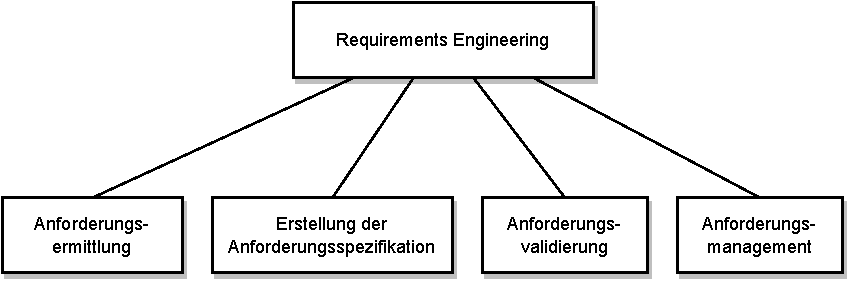
\includegraphics[width=\textwidth]{Bilder/Kapitel-6/aktivitaeten_requirements_engineering.pdf}
	\caption{Teilprozesse des Requirements Engineering}
	\label{fig:aktivitaeten_requirements_engineering}
\end{figure}

\vspace{\baselineskip} %%% für Druck

Der Prozess des Requirements Engineering kann in die vier Teilprozesse "`Anforderungsermittlung"', "`Erstellung der Anforderungsspezifikation"', "`Anforderungs-
\linebreak %%% für Druck
validierung"' und "`Anforderungsmanagement"' unterteilt werden (s.~Abb.~\ref{fig:aktivitaeten_requirements_engineering}). In allen vier Teilprozessen kommt der Begriff \textit{Anforderung} vor.

Abschnitt~\ref{sec:Kap-6.2} wird sich nachher detaillierter mit Anforderungen, ihren Quellen, ihren Beziehungen und den Möglichkeiten, sie zu kategorisieren, beschäftigen. An dieser Stelle sagen wir erstmal allgemein: \marginline{Anforderung}
Eine Anforderung ist etwas, das \textbf{„jemand“} von dem (zukünftigen) Softwareprodukt erwartet, um ein bestimmtes Problem lösen oder ein bestimmtes Ziel erreichen zu können. Und wir beginnen dieses Kapitel mit dem „jemand“, die oder der eine Anforderung stellt -- dem sogenannten Stakeholder.



% 6.1
\clearpage
\section{Stakeholder, Ziele und Produktumfang}
\label{sec:Kap-6.1}

Den Begriff \textit{Stakeholder} -- für den es wie für den Begriff Requirements Engineering keine hundertprozentig adäquate deutsche Übersetzung gibt -- hatten wir in Abschnitt~1.2.2 % TODO Abschnitt~\ref{sec:Kap-1.3.2}
bereits erwähnt. Er umfasst alle Personen(gruppen), deren Interessen in irgendeiner Weise durch das zu entwickelnde Softwareprodukt berührt werden oder die Einfluss auf die Erstellung des Produkts nehmen können. Im Hinblick auf Require\-ments Engineering bedeutet das, dass diese Personen (mittelbar oder unmittelbar) Anforderungen an das Softwareprodukt stellen (können).  

Doch längst nicht alle Bedürfnisse der Stakeholder sind relevant für das konkret zu entwickelnde Softwareprodukt. Die \textbf{Stakeholder} und ihre Bedürfnisse müssen in Einklang gebracht werden mit den \textbf{(Unternehmens)Zielen}, die durch den Einsatz des Softwareprodukts erreicht werden sollen und dem Aufgabenfeld (der so genannte \textbf{Produktumfang}, engl. scope), das die zukünftige Software abdecken soll: 

\begin{itemize}[
		label={\sttpHervorhebung{$\Rightarrow$}},
		]
	\item Die Ziele, 
		\marginline{der Zirkel aus Stakeholdern, Zielen und Produktumfang}
		die mit dem Einsatz des Softwareprodukts erreicht werden sollen, sind die Grundlage für den Produktumfang. Letzterer gibt an, für welche Aufgabenbereiche das Softwareprodukt zuständig ist und für welche nicht. Abhängig vom Produktumfang sind unterschiedlich viele Gruppen von Stakeholdern vom Einsatz der Software betroffen und werden Anforderungen stellen. Die in das Softwareentwicklungsprojekt eingebundenen Stakeholder beeinflussen aber wiederum die Definition der Ziele, damit auch den Produktumfang, damit die Menge der Stakeholder usw. \cite[44]{rob13} nennt diesen Abhängigkeitszyklus „the trinity of scope, stakeholders, and goals“. 
\end{itemize}

In der Praxis können Ziele, Stakeholder und Produktumfang daher nicht isoliert voneinander betrachtet werden -- im Rahmen dieses Lerntexts werden wir es zugunsten der systematischen Darstellung in den folgenden Abschnitten trotzdem so handhaben. In der Praxis wird man mit einem der drei Aspekte beginnen -- meistens hat der Auftraggeber zumindest eine grobe Vorstellung vom gewünschten Produktumfang -- und alle drei iterativ so lange anpassen, bis sie stimmig sind. Unabhängig davon, in welcher Reihenfolge und wie stark parallelisiert die Bestimmung von Zielen, Stakeholdern und Produktumfang in einem Softwareentwicklungsprojekt stattfindet: Vor der systematischen Ermittlung von Anforderungen an das Softwareprodukt sollten diese drei Analysen abgeschlossen oder zumindest weit fortgeschritten sein. Andernfalls ist die Wahrscheinlichkeit hoch, dass für die Ermittlung zu vieler, und auch später nicht berücksichtigter Anforderungen unnötig Ressourcen investiert wurden.

Abbildung~\ref{fig:stakeholder_ziele_produktumfang_anfoderungen} zeigt den Zusammenhang zwischen Zielen, Stakeholdern und Produkt\-umfang auf der einen Seite und den Anforderungen auf der anderen Seite:

\begin{itemize}
	\item Die \textbf{\sttpHervorhebung{Bedürfnisse}} der Stakeholder \textbf{\sttpHervorhebung{manifestieren sich in den Anforderungen}}. Insofern bilden die Bedürfnisse der Stakeholder die Basis für die Anforderungen.
	\item Der \textbf{\sttpHervorhebung{Produktumfang}} ist der \textbf{\sttpHervorhebung{Rahmen}}, in den die Anforderungen passen müssen. Die Anforderungen müssen also zu dem vom Produktumfang definierten Aufgabenbereich gehören.
	
	\pagebreak %%% für Druck
	
	\item Die \textbf{\sttpHervorhebung{Ziele}} sind der \textbf{\sttpHervorhebung{Maßstab für die Relevanz}} der Anforderungen. Das bedeutet, dass jede im Softwareentwicklungsprojekt berücksichtigte Anforderung zur Erfüllung mindestens eines der Ziele des Projekts beitragen muss.
\end{itemize}

\begin{figure}[!t]
	\vspace{\baselineskip} %%% für Druck
	\centering
	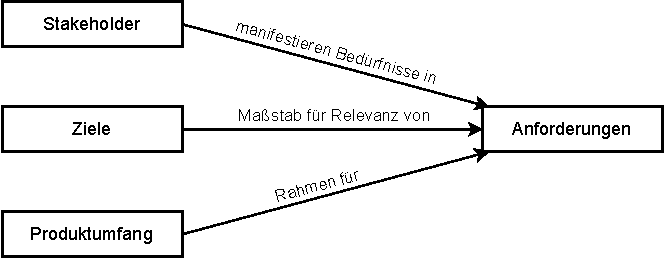
\includegraphics{Bilder/Kapitel-6/begriffe-version1.pdf}
	\caption{Stakeholder, Ziele, Produktumfang und Anforderungen}
	\label{fig:stakeholder_ziele_produktumfang_anfoderungen}
\end{figure}

Beispiel aus einer IT-fernen Lebenswelt: Der römische Staatsmann Cato der Ältere (234-149 v. Chr.) soll alle seine Reden im Senat -- unabhängig vom Thema -- mit dem Ausspruch beendet haben: „Im Übrigen bin ich der Meinung, dass Karthago zerstört werden muss“. In dieser Anekdote ist die Zerstörung Karthagos (in der Antike ein einflussreicher Stadtstaat in Nordafrika und Gegner des Römischen Reichs) ein Bedürfnis des Stakeholders Cato, das als Anforderung „Karthago muss zerstört werden“ dokumentiert werden könnte. In einer Senatssitzung, die sich mit der Verbesserung landwirtschaftlicher Methoden beschäftigt, steht eine solche Anforderung komplett abseits des Themas. In einer Senatssitzung, die sich mit den Beziehungen zwischen dem Römischen Reich und anderen Reichen beschäftigt, würde man sie kontrovers diskutieren. Die identische Anforderung befindet sich in dem einen Fall also außerhalb, in dem anderen Fall innerhalb des definierten Aufgabenbereichs des Senats. Betrachten wir den letzteren Fall. Die Relevanz der Anforderung misst sich an den Zielen des entsprechenden Vorhabens. Wenn das Ziel des römischen Senats die Aushandlung von Bündnissen mit anderen Reichen ist, sollte Catos Anforderung der Zerstörung Karthagos besser unberücksichtigt bleiben, da sie nicht zur Erfüllung des Ziels beiträgt. Wie es endete zwischen Cato und Karthago beschreibt \linebreak 
{\small [\url{https://de.wikipedia.org/wiki/Ceterum_censeo_Carthaginem_esse_delendam}]}.

In den folgenden Abschnitten werden wir uns mit den Themen Stakeholder, Ziele und Produktumfang und ihrem Einfluss auf die Anforderungsermittlung detaillierter beschäftigen. 
\subsection{Stakeholder}
\label{sec:Kap-6.1.1}

Es ist durchaus nicht trivial, mit einem Softwareprodukt die Bedürfnisse der zukünftigen Nutzer zu treffen. Denn in der Regel wird es nicht nur für eine Nutzergruppe, sondern für eine Menge sehr heterogener Teilgruppen mit eventuell widerstreitenden Bedürfnissen entwickelt. Zum Beispiel könnten bei den zukünftigen Nutzern unterschiedliche fachliche Hintergründe bzw. Arbeitsschwerpunkte vorliegen (wie \zb im Zookontext Tierpfleger, Mitarbeiter an der Zookasse, Verwaltungsmitarbeiter, IT-Personal) oder die Gruppen könnten unterschiedlich viel Erfahrung im Umgang mit Software haben. Ein anderer Unterschied könnte darin bestehen, wie lange oder wie intensiv jemand das Softwareprodukt täglich einsetzen muss. 

Um von konkreten Personen (\zb Tierpfleger Helmut, der sehr IT-erfahren ist und das Softwareprodukt ca. eine halbe Stunde pro Tag nutzen wird) zu abstrahieren, verwendet man auch im Requirements Engineering den Begriff der Rolle, \marginline{Rolle}
den wir schon im Kontext der Zusammensetzung des Entwicklungsteams in Abschnitt 1.2.2 % TODO Abschnitt~\ref{sec:Kap-1.3.2}
vorgestellt hatten. Im Rahmen des Requirements Engineering geht es allerdings nicht um Rollen während der \textbf{Entwicklung} des Softwareprodukts, sondern um eingenommene Rollen bei dessen \textbf{Nutzung}. Unterschiedliche Rollen stellen unterschiedliche Anforderungen an das Softwareprodukt, zum Beispiel weil sie verschiedene Funktionalitäten nutzen werden (\zb Rolle Tierpfleger vs. Rolle Mitarbeiter der Zoo\-verwaltung) oder die Software für sie unterschiedlich stark intuitiv zu nutzen sein muss (\zb Rolle IT-erfahrener Nutzer vs. Rolle IT-unerfahrener Nutzer).

Die verschiedenen (zukünftigen) Nutzerrollen sind jedoch bei Weitem nicht die einzigen Stakeholder, die Anforderungen an das Softwareprodukt stellen werden. Zu den im Requirements Engineering relevanten Stakeholdern gehören eine Reihe weiterer Personengruppen, darunter auch solche, die das Softwareprodukt später gar nicht selber nutzen werden. Mögliche Stakeholder eines Softwareentwicklungsprozesses im Rahmen des Requirements Engineering sind:

\begin{itemize}
	\setlength{\itemsep}{0.4mm} %%% für Druck
	
	\item \textbf{Nutzer des Softwareprodukts}: wie beschrieben, handelt es sich häufig um eine sehr heterogene Gruppe mit unterschiedlichen, teilweise auch wider\-streitenden Interessen. Die Anforderungen der Nutzer beziehen sich in der Regel auf das Vorhandensein gewünschter Funktionalitäten und auf Aspekte wie die einfache Bedienbarkeit der Software.
	\item \textbf{Führungsebene des Auftraggebers}: diejenigen Personen(gruppen), die entscheiden, dass das Softwareentwicklungsprojekt durchgeführt wird und Ressourcen für das Projekt bewilligen. Wenn es sich nicht um eine Auftragsarbeit, sondern um eine Entwicklung für die eigene Institution bzw. eine Entwicklung zum Verkauf auf dem kommerziellen Markt handelt, handelt es sich bei diesem Stakeholder um die Führungsebene des eigenen Hauses. Dieser Stakeholder definiert, welche (Unternehmens)Ziele durch das zu entwickelnde Softwareprodukt erreicht werden sollen und er entscheidet zum Beispiel auch, welche Mitarbeiter als Domänenexperten für das Projekt abgestellt werden (können). Neben Anforderungen an den Entwicklungsprozess, wie die Einhaltung von Kosten- und Zeitplänen, könnte er auch konkrete Anforderungen an das Softwareprodukt stellen, zum Beispiel, dass dieses umfangreiche Hilfestellungen zu den einzelnen Funktionalitäten beinhalten muss, damit der spätere Schulungsaufwand für seine Mitarbeiter gering bleibt, oder dass es mit der bestehenden Hardware kompatibel sein muss, damit nicht neue Hardware für die Mitarbeiter gekauft werden muss.
	\item \textbf{IT-Abteilung des Auftraggebers}: Diesem Stakeholder könnte wichtig sein, dass das neue Produkt gut in die Haus-IT eingepasst werden kann, zum Beispiel indem es entsprechende Schnittstellen zu anderen verwendeten Softwareprodukten im Haus hat. Des Weiteren werden aus dieser Richtung Anforderungen im Hinblick auf Betrieb und Wartung des zukünftigen Softwareprodukts kommen.
	\item \textbf{Verwaltung des Auftraggebers}: Der Einsatz des neuen Produkts kann auch Auswirkungen auf Bereiche außerhalb der Fachabteilungen, für die es gedacht ist, haben. Wenn zum Beispiel im Zookontext die Futterbeschaffung für die
	\linebreak %%% für Druck
	Tiere bisher von den einzelnen Tierpflegern übernommen wurde und jetzt mit der neuen Software zentral organisiert werden soll, ändern sich Arbeits\-prozesse im Einkauf. Die dortigen Mitarbeiter werden entsprechend Anforderungen (\zb die Speicherung verwaltungsrelevanter Informationen) an das Softwareprodukt stellen.
	\item \textbf{Marketing/ Öffentlichkeitsarbeit/ Pressestelle etc. des 
	Auftrag- \linebreak
	gebers}: Dieser Stakeholder wird nach Möglichkeiten suchen, wie das neue Produkt in die Öffentlichkeitsarbeit des Unternehmens eingebunden werden kann bzw. diese vereinfachen kann. Wenn ein Produkt für den kommerziellen Markt entwickelt wird, nimmt dieser Stakeholder eine besonders zentrale Rolle ein, aber auch bei der (individualisierten) Entwicklung für einen Auftraggeber oder für das eigene Haus können Anforderungen aus dieser Richtung kommen. Zum Beispiel könnte die Pressestelle des Zoos die Anforderung stellen, dass das Softwareprodukt automatisiert bei jeder Geburt im Zoo eine entsprechende Pressemitteilung an die regionalen Zeitungen versendet.
	\item \textbf{Mitarbeiter der Qualitätssicherung des Auftraggebers}: Von diesem Stakeholder sind Anforderungen bezüglich der Einhaltung von (unternehmenseinheitlichen) Prozessen und Standards, aber -- bezogen auf das Software\-produkt -- auch Anforderungen zur Bedienbarkeit der Software und zum Vorhandensein spezifischer Testfälle, die Qualitätskriterien der Software über\-prüfen, zu erwarten.
	\item \textbf{Betriebsrat des Auftraggebers}: Dieser Stakeholder könnte zum Beispiel Anforderungen bzw. Bedingungen formulieren, welche Informationen die Software erheben darf, wenn Mitarbeiter sie nutzen. Zudem werden durch die mögliche Änderung von Arbeitsprozessen durch das Softwareprodukt die \mbox{Interessen} dieses Stakeholders berührt.
	\item \textbf{Kunden des Auftraggebers}: wie zum Beispiel im Zookontext die Besucher des Zoos. Auch die Bedürfnisse dieser Gruppe sollten nicht unberücksichtigt bleiben, denn sie werden häufig der Grund sein, weshalb der Auftraggeber überhaupt ein Softwareprodukt entwickeln bzw. verbessern lassen möchte. In der Regel werden die Kunden des Auftraggebers nicht direkt an der Anforderungsermittlung mitwirken, sondern der Auftraggeber muss ihre Bedürfnisse mitdenken (vielleicht sogar durch Befragungen oder Ähnliches im Vorfeld erhoben haben) und -- sofern sie zu seinen Zielen passen -- als Anforderungen an das Softwareprodukt formulieren.
	\item \textbf{Betriebliche oder staatliche Datenschutzbeauftragte}: Aus dieser Richtung sind vor allem Anforderungen zu den von der Software verarbeiteten Daten zu erwarten. In Bereichen, in denen besonders schützenswerte personenbezogene Daten verarbeitet werden (\zb Software im Gesundheitsumfeld) hat dieser Stakeholder eine besonders zentrale Rolle. Aber auch das im Zoobeispiel von der Zoodirektorin vorgesehene Veröffentlichen der Namen der Tierpfleger berührt schon die Interessen dieses Stakeholders.
	\item \textbf{Aufsichtsbehörden/ Prüfer/ Sicherheitsexperten}: Je nach Domäne und Einsatzzweck des Softwareprodukts müssen unterschiedlich strenge gesetzliche Vorschriften eingehalten werden. Entsprechende Anforderungen von diesem Stakeholder werden nicht nur von konkreten Personen gestellt, sondern finden sich auch in Gesetzen und Richtlinien, die das Softwareentwicklungsprojekt berücksichtigen muss.
	\item \textbf{Schulungs- und Servicepersonal des Auftraggebers oder Auftrag\-nehmers}: Diese Personen haben die Aufgabe, die Nutzer in der Verwendung des Softwareprodukts zu schulen und ihnen bei Problemen zu helfen. Unabhängig davon, ob dieser Stakeholder beim Auftraggeber angesiedelt ist oder bei dem Unternehmen, das das Softwareprodukt erstellt hat, wird er Anforderungen in Bezug auf die einfache Bedienbarkeit der Software und auf das Vorhandensein von Dokumentationen zur Software stellen.
	\item \textbf{Auftragnehmer}: Auch das Unternehmen, das das Softwareprodukt erstellt, bzw. bei Eigenentwicklung die entsprechende Abteilung, kann ein 
	Stake- \linebreak %%% für Druck
	holder im Softwareentwicklungsprozess sein. Das kann Beschränkungen bezüglich möglicher Programmiersprachen oder Entwicklungstechniken für das Software\-produkt betreffen, zum Beispiel kann evtl. nicht in C$++$ implementiert werden, wenn das Personal nur aus Java-Entwicklern besteht. Es könnte von diesem Stakeholder aber auch gewünscht sein, zu entwickelnde Komponenten möglichst wiederverwendbar zu gestalten, um sie auch in anderen Softwareentwicklungsprojekten einsetzen zu können. Letztere Anforderung wird häufig nicht explizit formuliert werden, insbesondere wenn für einen externen Auftraggeber entwickelt wird oder eine solche Anforderung an eine Komponente mit Anforderungen anderer Stakeholder kollidieren würde.
\end{itemize}

Es ist sehr projektspezifisch, welche Gruppen genau zu den Stakeholdern gehören. Neben den Zielen und dem Produktumfang der zukünftigen Software ist dies auch abhängig von der Domäne sowie der Struktur und Größe des Unternehmens des Auftraggebers (\zb hat nicht jedes Unternehmen einen Qualitätssicherungsexperten und vielleicht auch keine eigene IT-Abteilung). Zudem werden nicht alle Stakeholder für das Gelingen des Projekts gleich wichtig sein. In jedem Fall gibt es für ein Softwareentwicklungsprojekt aber oft deutlich mehr zu berücksichtigende Stakeholder als man im ersten Moment denken würde.

Da alle diese Stakeholder potentielle Lieferanten von Anforderungen sind, ist es für das Softwareentwicklungsteam bzw. dessen Projektleiter wichtig, diese möglichst zu Beginn des Projekts zu kennen bzw. in Erfahrung zu bringen. Wenn Stakeholder unberücksichtigt bleiben, bleiben -- nicht immer, aber häufig -- auch deren Anforderungen unberücksichtigt. Und nach Murphys Gesetz (anything that \textbf{can} go wrong \textbf{will} go wrong) werden diese unberücksichtigten Anforderungen im späteren Projekt\-verlauf oder nach Einführung des Softwareprodukts doch prioritär werden und (unter Umständen umfangreiche und kostenintensive) Änderungen an der Software erforderlich machen. Insofern müssen (und werden) bei der Anforderungsermittlung nicht alle Stakeholder persönlich anwesend sein, aber ihre Interessen sollten immer mit am Tisch sitzen. In der Praxis gibt es häufig von Seiten des Auftraggebers intern vor Projektstart abgestimmte Aufstellungen von Anforderungen, die schon die Interessen mehrerer Stakeholder vereinen und zumindest eine erste Basis für die Anforderungsermittlung bilden.

\vspace{1.5mm} %%% für Druck

Die \marginline{Konflikt\-potenzial} Berücksichtigung und Priorisierung der Anforderungen verschiedener Stake\-holder kann enormes Konfliktpotenzial bieten, insbesondere dann, wenn mit den vorgesehenen Ressourcen nicht alle Anforderungen umgesetzt werden können oder sich Anforderungen verschiedener Stakeholder nicht miteinander vereinbaren lassen. Hinzu kommt, dass Stakeholder neben den Interessen, die sich aus ihrer Position oder ihren Arbeitsschwerpunkten ergeben, auch persönliche Interessen haben, die mit\-unter ihren Weg in die Anforderungen finden. Zum Beispiel könnten sich Mitarbeiter wünschen, dass das zukünftige Softwareprodukt sie von lästigen Routineaufgaben befreit und entsprechende Anforderungen höher priorisieren als es den eigentlichen Zielen des Softwareentwicklungsprojekts entspricht. Auf der anderen Seite könnten zukünftige Nutzer versuchen, alle Funktionalitäten zu verhindern, die ihre bisherigen Arbeitsprozesse verändern. Aus Sicht des Entwicklungsteams des Softwareprodukts ist es zentral, dass es ganz klare Regeln gibt, welche Mitarbeiter des Auftraggebers direkt Anforderungen stellen oder priorisieren dürfen und welche ihre Interessen dem Entwicklungsteam nur indirekt über festgelegte Ansprechpartner des Auftraggebers mitteilen können. Diese Entscheidung trifft die Führungsebene des Auftraggebers bzw. ein von ihr benannter Entscheidungsträger. Meistens ist es allerdings keine gute Option, allen anderen Personen des Unternehmens den Zugang zum Entwicklungsteam zu verweigern, da letzterem damit auch Quellen für Domänenwissen vorenthalten werden könnten. Zumal es in der Praxis auch nicht selten vorkommt, dass der benannte Ansprechpartner für das Entwicklungsteam die Domäne deutlich weniger gut kennt als andere Mitarbeiter des Unternehmens.

\vspace{\baselineskip} %%% für Druck

\minisec{Stakeholderpflege in agilen Projekten}

Die frühe Kenntnis der potenziellen Stakeholder ist auch in agilen Softwareentwicklungsprojekten sehr wichtig, auch wenn diese die Möglichkeit von Anforderungs\-änderungen über die komplette Projektlaufzeit vorsehen. Die Schwierigkeit liegt hier weniger darin, dass \textbf{überhaupt} neue Anforderungen gestellt werden. Diese können (mit mehr oder weniger Anpassungen am bestehenden Programmcode) in späteren Iterationen umgesetzt werden. Problematisch kann es aber werden, wenn neue Stake\-holder die schon bearbeiteten Anforderungen oder die Art und Weise wie diese umgesetzt wurden, \textbf{grundsätzlich} in Frage stellen. 

\vspace{1.5mm} %%% für Druck

Das agile Vorgehensmodell Scrum geht einen sehr rigorosen Weg, um die möglichen Zielkonflikte zwischen Stakeholdern vom Entwicklungsteam fernzuhalten. Die \marginline{die Rolle Product Owner} Rolle des Product Owner, der die Anforderungen priorisiert, wird nur von genau einer (vom Auftraggeber zu benennenden) Person übernommen. Von der fachlichen Seite bestimmt nur der Product Owner, welche Anforderungen in der nächsten Iteration umgesetzt werden sollen. In der Praxis wird der Product Owner zwar weitere Mit\-arbeiter des Auftraggebers einbinden (müssen), indem er diese Anforderungen formulieren lässt oder sie sogar als Domänenexperten direkt mit ins Projekt einbezieht. Entscheider aus Sicht des Entwicklungsteams bleibt aber ausschließlich der Product Owner, unabhängig davon wie viele andere Personen an Besprechungen teilnehmen, Ideen oder Anforderungen äußern. Die Rolle Product Owner ist kein einfacher Job. Sie muss jederzeit den Überblick über das Gesamtprodukt haben und wissen, welche Anforderungen die höchste Priorität erhalten sollen, die Fragen der Entwickler zur Domäne und zu den Anforderungen beantworten können bzw. Personen benennen können, die dazu in der Lage sind, dabei die Interessen aller Stakeholder berücksichtigen und deren Konflikte lösen und gleichzeitig ihrer Führungsebene regelmäßig über den Stand des Projekts berichten.

\vspace{\baselineskip} %%% für Druck

\minisec{Identifizieren und Dokumentieren der Stakeholder}

Es gibt in der Literatur zahlreiche praktische Hinweise und Methoden, wie sich die Stakeholder für ein Softwareentwicklungsprojekt bestimmen lassen, wie man ihre Interessen und Ziele dokumentieren kann und wie sich die Wichtigkeit einzelner Stakeholder bewerten lässt.

\begin{figure}[h!]
	\centering
	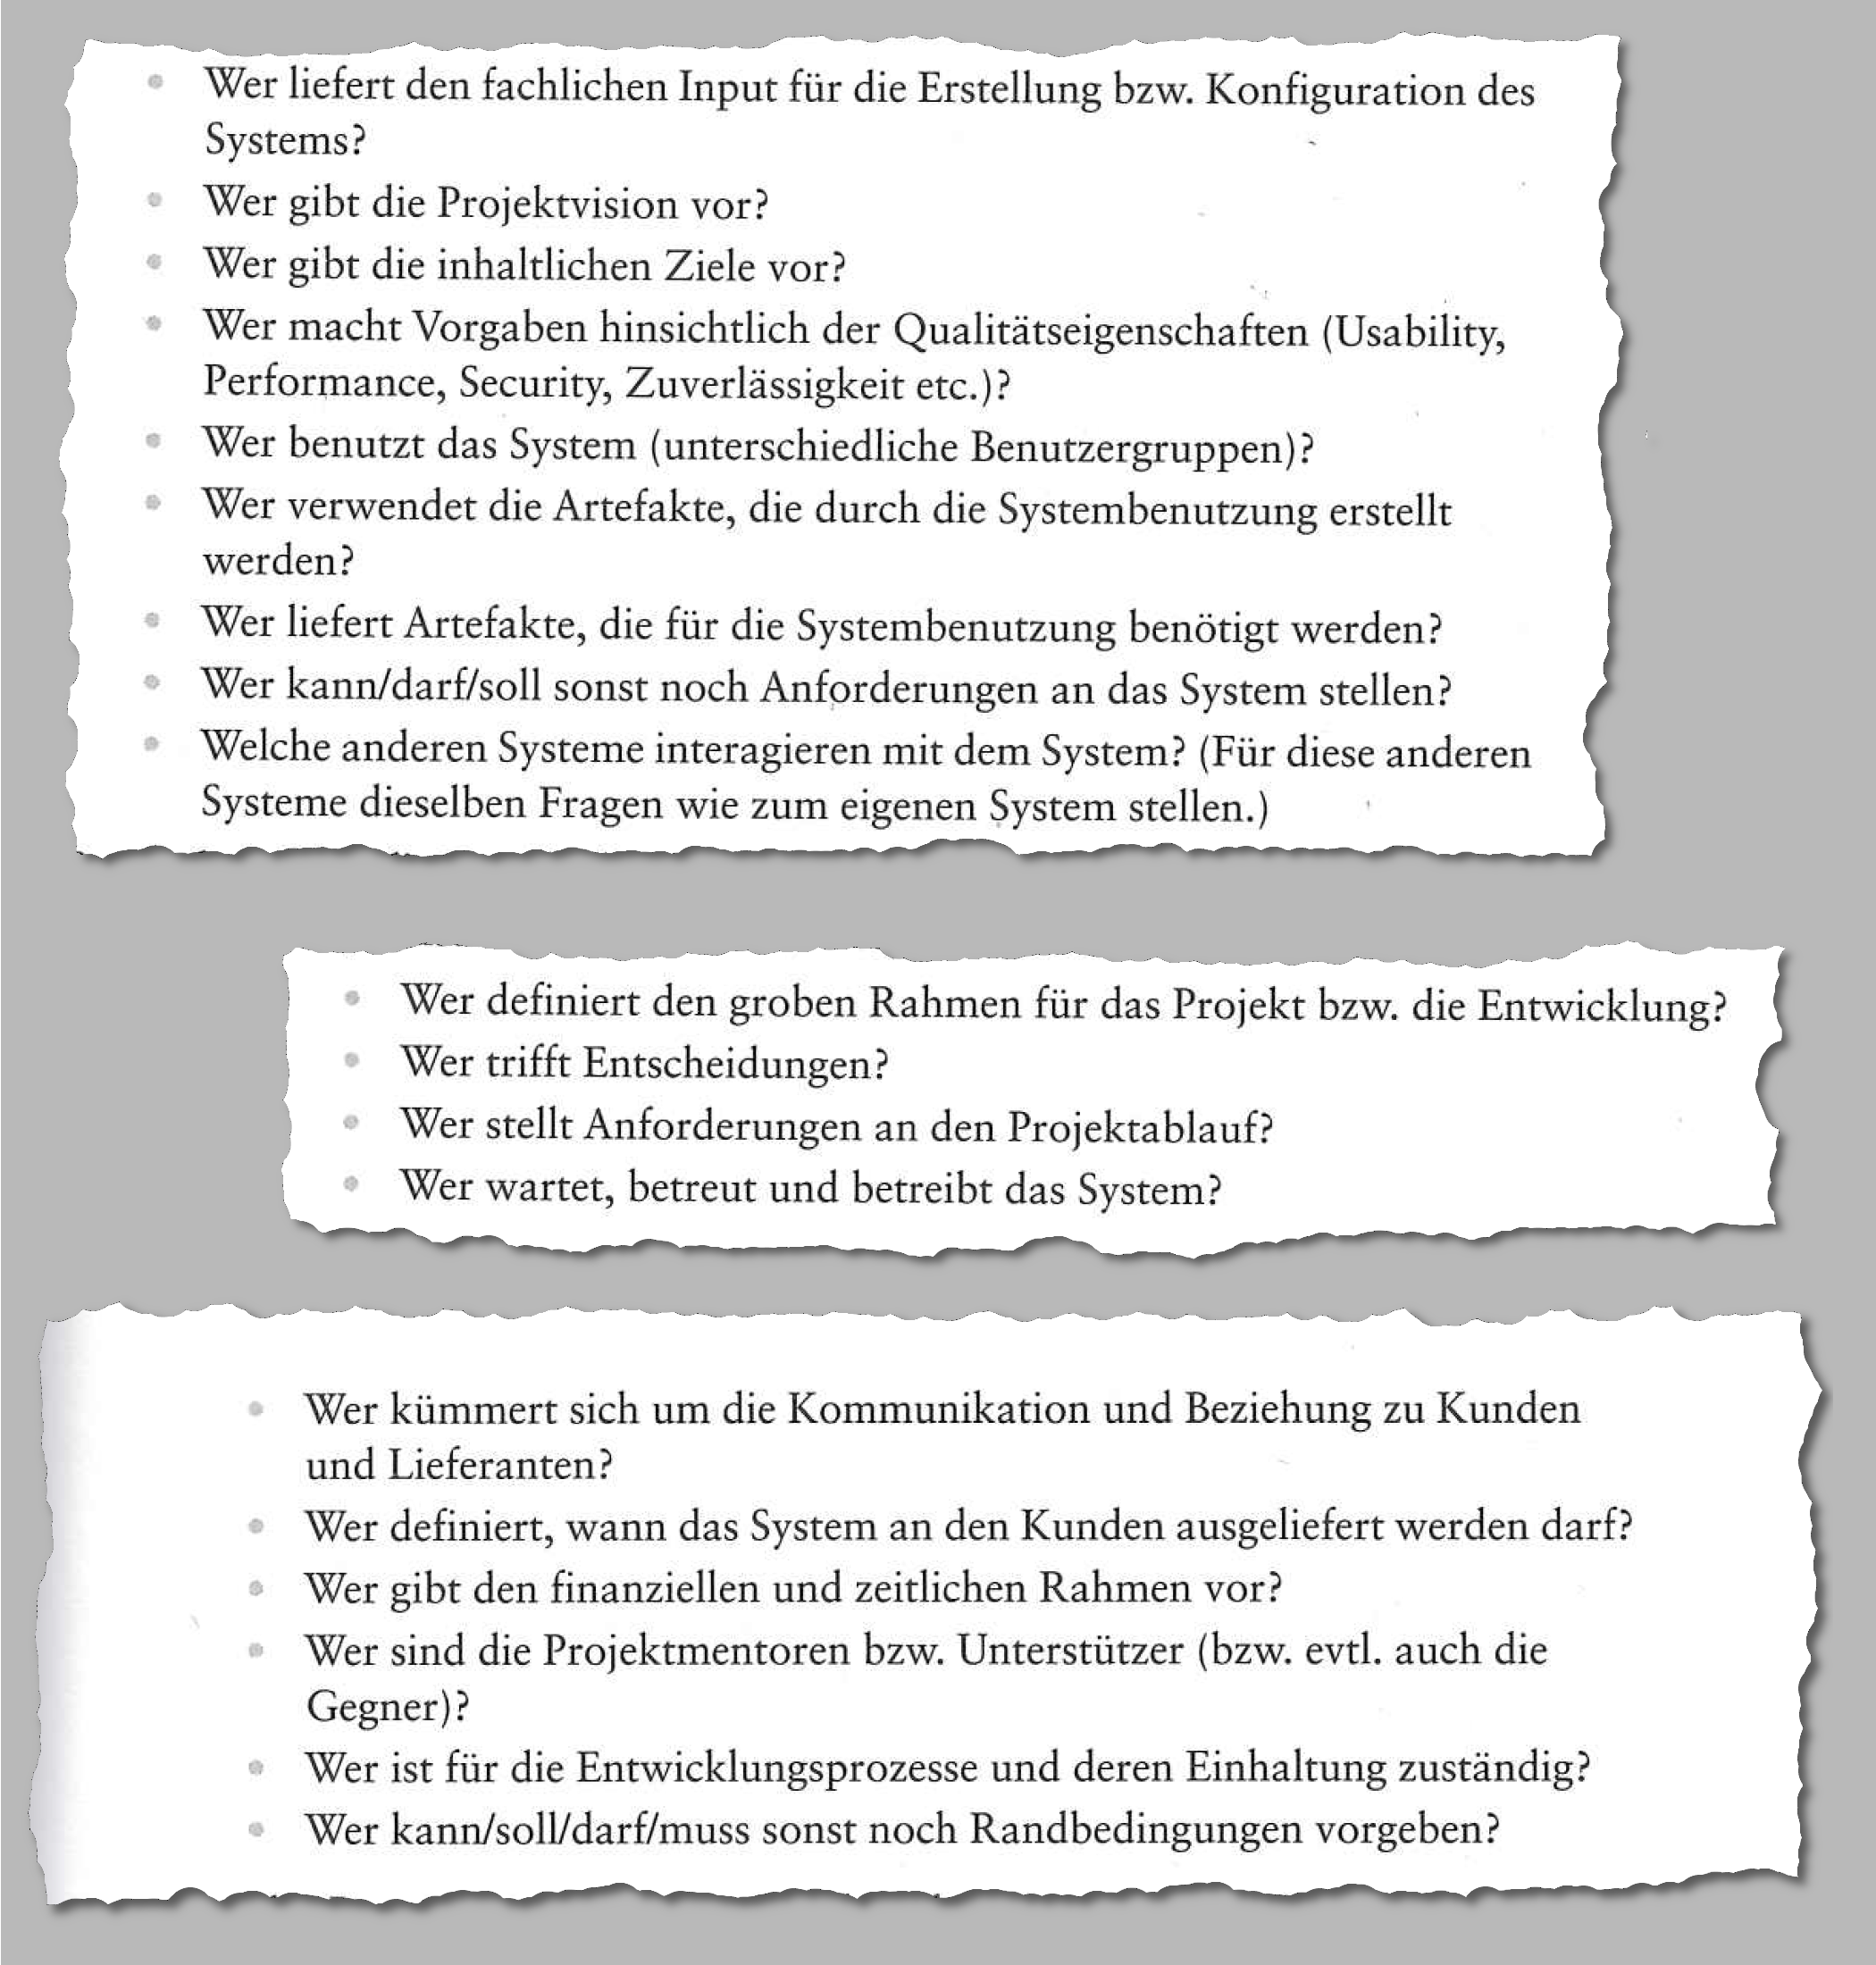
\includegraphics[width=\textwidth]{Bilder/Kapitel-6/Stakeholder_Medley_V2.png}
	\caption[Mögliche Fragen zur Identifizierung von Stakeholdern]{Mögliche Fragen zur Identifizierung von Stakeholdern. Inhalte aus: \cite[84 \psq]{ber18}}
	\label{fig:stakeholder_medley}
	
	\vspace{\baselineskip} %%% für Druck
\end{figure}

Eine Möglichkeit, Stakeholder zu bestimmen, ist dem vom Auftraggeber genannten Ansprechpartner schematische Fragen der Art, „Wer wartet und betreut das zukünftige System?“, „Wer definiert die inhaltlichen Ziele?“, „Wer bestimmt üblicherweise den Projektablauf durchzuführender Projekte?“ zu stellen und auf diese Weise \mbox{Namen} von weiteren Mitarbeitern oder Hinweise auf Organisationseinheiten des Unternehmens zu erhalten, die potenzielle Stakeholder sein könnten. Abbildung~\ref{fig:stakeholder_medley} zeigt Ausschnitte aus Fragenlisten von \cite[84 \psq]{ber18}. Weitere Listen solcher Fragen, an denen man sich orientieren kann, finden Sie bei \cite[36]{lap17} und \cite[122 \psqq]{lef11}.

Bei \cite[55 \psqq]{ebe22} finden 
\marginline{weiterführende Literatur}
Sie eine praktische Stakeholder-Analyse in acht Schritten, mit der Stakeholder, ihre Interessen und Konfliktpotenziale zwischen Stake\-holdern identifiziert und dokumentiert werden können. \cite[44 \psq]{rob13} stellt mit der sogenannten Stakeholder Map zudem eine Möglichkeit vor, Stakeholder und ihre Beziehungen zueinander in größeren Einheiten zu kategorisieren und zu visualisieren. \cite[48 \psq]{oes13} stellt eine Methode zur Bewertung der Wichtigkeit eines Stakeholders vor, die das Risiko, diesen Stakeholder nicht zu  berücksichtigen und den benötigten Aufwand seine Interessen zu erkunden ins Verhältnis setzt. \cite[81 \psqq]{rup14} zeigt Beispiele für Schablonen zur Dokumentation von Stakeholdern, \mbox{ihren} Interessen und Einflussmöglichkeiten und stellt ein Stakeholder-Analysemodell vor, mit dem Stake\-holder anhand der Kriterien Einfluss und Motivation gruppiert werden können. \cite[121]{lef11} und \cite[46 \psq]{lap17} zeigen Beispiele für Stakeholder-
\linebreak %%% für Druck
Rankings. 

\subsection{Vision und Ziele}
\label{sec:Kap-6.1.2}

Die Ziele, die mit dem Einsatz des Softwareprodukts erreicht werden sollen, bilden den Maßstab für die Relevanz und damit die Berücksichtigung bzw. Nicht-Berücksichtigung der einzelnen geäußerten Anforderungen der verschiedenen Stakeholder. Vor den Zielen müssen wir uns zunächst mit der \textit{Vision} beschäftigen, die den Zielen auf einer höheren Abstraktionsebene vorgeschaltet ist.
\subsubsection{Vision}
\label{sec:Kap-6.1.2.1}

Im Rahmen des Requirements Engineering ist eine Produktvision (kurz: Vision, synonym: Systemidee) eine oft noch recht unkonkret formulierte Darstellung des Zustands, der mit dem Einsatz des Softwareprodukts erreicht werden soll. Die Vision soll vor allem deutlich machen, \textbf{warum} das Softwareentwicklungsprojekt (bzw. der Kauf einer Software) gestartet wird und inwiefern dadurch die aktuelle Situation verbessert wird. Im Einzelnen gehören zu einer Vision:

\begin{itemize}
	\item \textbf{\sttpHervorhebung{Die Darstellung der Ausgangslage und der Motivation für die 
			\linebreak %%% für Druck
			Projektdurchführung}}: Die Darstellung beinhaltet die Beschreibung der aktuellen Situation inklusiver bekannter Probleme (vor Einsatz des Produkts) und Erwartungen -- manchmal auch nur Hoffnungen --, inwiefern die \mbox{Situation} verbessert wird, wenn das Softwareprodukt eingesetzt wird. Hier geht es darum, den positiven Einfluss des einzuführenden Produkts in Bezug auf über\-geordnete Unternehmensziele, Arbeitsabläufe und das existierende Unter-
			\linebreak %%% für Druck
			nehmensumfeld zu skizzieren. 
	\item \textbf{\sttpHervorhebung{Eine skizzenhafte Beschreibung der Hauptcharakteristika des Softwareprodukts}}: Auf einem sehr hohen Abstraktionslevel werden die wichtigsten geplanten Eigenschaften und Funktionalitäten des Softwareprodukts beschrieben. Dazu können auch Einschränkungen gehören, welche Aufgaben\-bereiche nicht von der Software übernommen werden sollen (\zb wenn im Zoobeispiel die Verwaltung der Tierarztrechnungen nicht Bestandteil der \mbox{neuen} Zoo-Software sein sollte).
	\item \textbf{\sttpHervorhebung{Ein grober Überblick über Verbindungen zu anderen Systemen}}: Es sollte dargestellt werden, in welcher Umgebung das neue Softwareprodukt eingesetzt wird. Zu dieser Umgebung gehören andere im Unternehmen eingesetzte Softwareprodukte, zu denen zukünftig Schnittstellen existieren sollen. Es geht aber auch um die Einbindung des Softwareprodukts in existierende Geschäfts\-prozesse und um die Verbindungen zwischen dem neuen Produkt und der existierenden oder neu zu schaffenden Hardwareumgebung.
\end{itemize}

Aus der Vision werden durch Konkretisierung und Ausdifferenzierung der genannten Aspekte die Ziele des Softwareeinsatzes sowie Produktumfang und Systemkontext abgeleitet. Die Beschreibung der Hauptcharakteristika bildet zudem die Basis für die Spezifizierung der wichtigsten Komponenten des zukünftigen Produkts.

Visionen von Softwareprodukten können unterschiedliche Schwerpunkte setzen. Insbesondere im agilen Umfeld steht oft der Aspekt der Motivation im Vordergrund der Vision, während die Beschreibung der Hauptcharakteristika weniger Aufmerksamkeit bekommt. Bei Softwareentwicklungsprojekten, deren Inhalt die Ablösung eines existierenden Produkts durch eine neue Version bzw. ein neueres Produkt derselben Art ist, ergeben sich die gewünschten Charakteristika des neuen Produkts häufig aus den Problemen mit dem alten Produkt. In solchen Fällen findet man eher eine sehr knappe Beschreibung der Motivationslage und dafür schon recht konkrete Beschreibungen der Hauptcharakteristika.

Eine Vision kann unterschiedlich umfangreich sein, zum Beispiel auch nur wenige Sätze umfassen. In der Regel bewegt sich der Rahmen zwischen einer halben Seite und maximal zwei Seiten Umfang, \marginline{Formen von Visionen} wobei es sich nicht zwingend um klassische Textdokumente handeln muss. So kann auch über eine Kombination aus Stichpunkten und Grafiken am Whiteboard eine Vision kommuniziert werden. \cite[43 \psqq]{oes13} schlägt vor, für die Vision einen Produktkarton zu gestalten, wie man ihn als Verpackung eines realen (gegenständlichen) Produkts kennt. Auf diese Weise wird die Produktvision für alle Projektbeteiligten auch plastisch sichtbar. Gleichzeitig beschränkt der Produktkarton den Umfang der Vision und erfordert es, sie geeignet zu strukturieren, da man sich überlegen muss, welche Informationen auf welcher Seite des Kartons platziert werden sollen. Eine solche plastische Kommunikation der Vision ist auch im agilen Umfeld -- unter dem englischen Begriff vision boxing -- bekannt.

Der \marginline{abweichende Definitionen} Begriff Vision gehört zu den Begriffen im Softwareengineering, zu denen Sie von vier Autoren und Autorinnen vier verschiedene Definitionen erhalten. Ein sehr grundsätzlicher Unterschied besteht in der Beantwortung der Frage, ob Rahmenbedingungen und Restriktionen, wie die angesetzten Zeit- und Kostenbudgets für das Softwareentwicklungsprojekt oder vorgegebene Hardwareumgebungen für das zukünftige Softwareprodukt, Bestandteil der Vision sein sollten. Hier gilt für dieses Modul: Sie sind dann Bestandteil der Vision, wenn sie direkt das Softwareprodukt betreffen (\zb was soll das Softwareprodukt nicht tun; welche Qualitätsstandards sind einzuhalten) oder wenn sie sich auf die Umgebung beziehen, in der das Softwareprodukt eingesetzt werden soll (\zb welche Geschäftsprozesse dürfen nicht verändert werden; welche Einschränkungen existieren durch vorhandene Hardwarekomponenten). Rahmenbedingungen, die sich auf das Softwareentwicklungs\textbf{projekt} beziehen (\zb das Budget oder die Restriktion, dass der Softwarearchitekt dem Projekt nur zwei Tage pro Woche zur Verfügung steht) sind nicht Bestandteil der Vision. Sehr wohl aber müssen Vision und projektbezogene Rahmenbedingungen in Einklang gebracht werden, wenn das Projekt erfolgreich verlaufen soll. 

Ein weiterer Diskussionspunkt im Kontext des Vision-Begriffs ist, ob die Ziele des Einsatzes des Softwareprodukts ebenfalls Bestandteil der Vision sind. Aufmerksamen Leserinnen und Lesern dürfte nicht entgangen sein, dass unsere Antwort auf diese Frage \textbf{Nein} lautet: 

\begin{itemize}[
	label={\sttpHervorhebung{$\Rightarrow$}},
	]
	\item Die Vision ist die Basis, aus der (unter anderem) die Ziele abgeleitet werden. Vision und Ziele bewegen sich somit auf unterschiedlichen Abstraktions\-niveaus.
\end{itemize}

Abbildung~\ref{fig:von_vision_zu_anforderungen} zeigt eine Erweiterung der Abbildung~\ref{fig:stakeholder_ziele_produktumfang_anfoderungen} aus Abschnitt~\ref{sec:Kap-6.1}. Ergänzt ist hier zum einen der Begriff der Vision und sein Zusammenhang zu Zielen und Produktumfang. Zum anderen ist der Begriff des Systemkontexts hinzugekommen, mit dem wir uns in Abschnitt~\ref{sec:Kap-6.1.3} näher beschäftigen werden. 

\vspace{\baselineskip} %%% für Druck
\vspace{\baselineskip} %%% für Druck

\begin{figure}[h!]
	%\centering
	\begin{addmargin*}[0cm]{-\marginparwidth}
	\begin{addmargin*}[0cm]{-\marginparsep}
		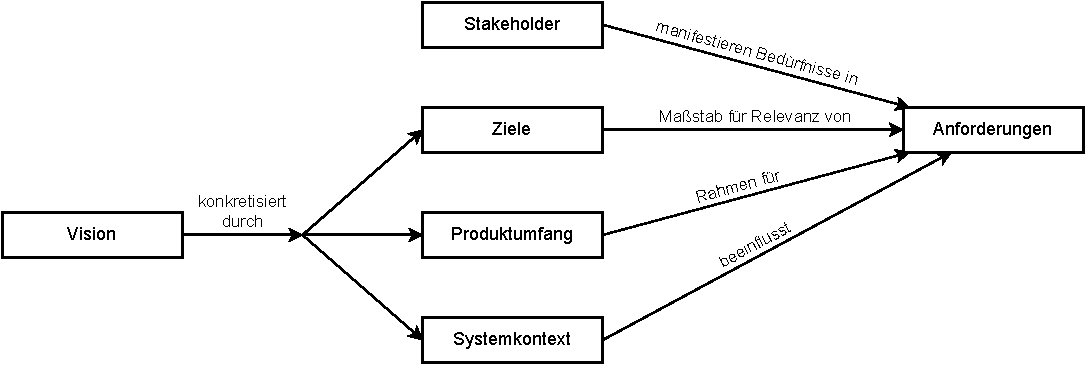
\includegraphics[scale=0.95]{Bilder/Kapitel-6/begriffe-version2.pdf}
		\caption{Von der Vision zu den Anforderungen}
		\label{fig:von_vision_zu_anforderungen}
	\end{addmargin*}
	\end{addmargin*}
\end{figure}

\pagebreak %%% für Druck

Wir \marginline{Sinn der Vision} möchten das Thema Vision mit der grundsätzlichen Frage abschließen: Wozu braucht man eine übergeordnete Vision, warum beginnt man nicht direkt mit der Formulierung von Zielen und Produktumfang?

\begin{itemize}[
	label={\sttpHervorhebung{$\Rightarrow$}},
	]
	\item Die Vision ist nötig, um die Produktziele, den Produktumfang und auch die Bedürfnisse der einzelnen Stakeholder des Projekts auf die übergreifenden Ziele, die aktuelle Situation und die Zukunftspläne des Unternehmens zu fokussieren. Wir erinnern daran, dass die Ziele der Maßstab für die Relevanz der Anforderungen sind. Der Maßstab für die Relevanz der einzelnen Ziele wiederum ist die Vision. Ähnliches gilt für den Produktumfang: Der Produktumfang ist der Rahmen, in den die Anforderungen passen müssen. Der Rahmen, in den der Produktumfang passen muss, ist die Vision. 
\end{itemize}
\subsubsection{Ziele}
\label{sec:Kap-6.1.2.2}

Die Darstellung der Vision beinhaltet, welche grundsätzlichen Verbesserungen durch den Einsatz des neuen Softwareprodukts erwartet werden. Die Beschreibung der Ziele konkretisiert diese Darstellung, indem genauer spezifiziert wird, in welchen Bereichen und bei welchen Aspekten, in welchem Umfang eine Verbesserung angestrebt wird. Sinnvoll ist es, nur Sollzustände zu beschreiben anstelle der Wege zur Erreichung dieser Sollzustände. \marginline{lösungsneutrale Ziele} Ziele sollten daher weitgehend \textit{lösungsneutral} formuliert werden, damit mögliche Lösungen durch die Formulierung des Ziels nicht von Beginn an ausgeschlossen werden. Zum Beispiel sollte das Ziel einer gemeinsamen Datenhaltung für die verschiedenen interagierenden Softwareprodukte des Unternehmens nicht durch die Vorgabe der Datenbanktechnologie (\zb relational, dokumenten\-orientiert) unnötig eingeschränkt werden. Es kann aber (gesetzliche, unternehmerische, arbeits\-organisa\-torische etc.) Rahmenbedingungen für den Betrieb des Softwareprodukts geben, die nicht ignoriert werden können und dementsprechend Teil der Ziel\-formulierung sein müssen, auch wenn sie die möglichen Lösungswege zur Erreichung eines Ziels einschränken. Im Beispiel von eben könnte es aus datenschutzrechtlichen oder sicherheitstechnischen Gründen notwendig sein, dass die Datenhaltung innerhalb des Unternehmens erfolgt und damit zum Beispiel externe Cloud-basierte Lösungen für die Erreichung des Ziels von vornherein wegfallen.

Neben der Lösungsneutralität bei gleichzeitiger Berücksichtigung relevanter Rahmen\-bedingungen sollte die Formulierung von Zielen für den Einsatz eines Software\-produkts bestimmten weiteren Qualitätskriterien genügen. Im Rahmen des Require\-ments Engineering werden dafür unterschiedliche Kriterienlisten aufgestellt (\zb \cite[S. 26 und S. 84]{rup14} oder \cite[457 \psqq]{bal09}), die verschiedene Schwer\-punkte setzen, sich im Großen und Ganzen aber sehr ähnlich sind. Verbreitet ist die Anwendung des ursprünglich aus dem Bereich der Mitarbeiterführung stammenden und auch im Projektmanagement bei Projekten außerhalb der IT häufig eingesetzten SMART-Katalogs. Das Akronym SMART 
\marginline{SMART} 
steht für \textbf{\sttpHervorhebung{S}}pecific, \textbf{\sttpHervorhebung{M}}easurable, \textbf{\sttpHervorhebung{A}}chievable, \textbf{\sttpHervorhebung{R}}easonable, \textbf{\sttpHervorhebung{T}}ime-Bound\footnote{Insbesondere für die Buchstaben A und R findet man in der Literatur teilweise auch andere Begriffe mit abweichender Bedeutung. Die inhaltliche Bedeutung des Gesamtakronyms ist aber im Großen und Ganzen unbestritten.}.  Ziele sollten danach folgende Kriterien aufweisen:

\begin{itemize}
	\item \textbf{Specific (spezifisch, gezielt, bestimmt)}: Ziele sollten eindeutig und so präzise wie möglich formuliert sein und vollständig beschrieben werden. Es muss deutlich werden, auf welchen Aspekt (\zb welcher Erfolgsfaktor) sich die angestrebte Verbesserung bezieht. Zum Beispiel wäre „die Relevanz des Zoos erhöhen“ nicht spezifisch genug, da unklar bleibt, an welchen Stellschrauben gedreht werden müsste. Spezifisch formulierte Ziele in diesem Zusammenhang wären zum Beispiel „das jährliche Besucheraufkommen erhöhen“ oder „Ausweitung der Öffentlichkeitsarbeit“. Das Kriterium spezifisch beinhaltet auch, dass ein Ziel für alle Stakeholder verständlich ist. Es kann und es wird Unstimmigkeiten zwischen verschiedenen Stakeholdern über die Priorität eines Ziels geben, es dürfen aber keine Missverständnisse über den Inhalt des entsprechenden Ziels bestehen.

	\vspace{2.3mm} %%% für Druck

	\item \textbf{Measurable (messbar)}: Die Erreichung eines Ziels sollte überprüfbar und im Idealfall der Grad der Zielerreichung messbar sein. Man sollte also angeben können, ab wann das Ziel als erreicht gelten soll. Das setzt voraus, dass die Formulierung des Ziels messbare Parameter enthält und entsprechende Metriken festgelegt werden. Um das Ziel „das jährliche Besucheraufkommen erhöhen“ messbar zu formulieren, benötigt man wenigstens die Angabe des Ausgangspunkts, zum Beispiel „im Vergleich zum letzten Jahr“ oder „im Vergleich zum durchschnittlichen Besucheraufkommen der letzten fünf Jahre“. Idealerweise sollte man in diesem Beispiel auch noch spezifizieren, wie stark das Besucheraufkommen steigen soll („um 10\% im Jahresdurchschnitt“, „um 20 Besucher pro Tag“ etc. ), denn ansonsten würde auch durch einen einzigen Besucher mehr pro Jahr das Ziel erfüllt werden. Und dafür würde sich der personelle und finanzielle Aufwand der Entwicklung des Softwareprodukts sicher nicht lohnen. 
	
	\vspace{2.3mm} %%% für Druck

	\item \textbf{Achievable (erreichbar, realisierbar, umsetzbar)}: Ein Ziel muss mit den vorhandenen Ressourcen, in der zur Verfügung stehenden Zeit (\su Kriterium Time-Bound) und unter den gegebenen Rahmenbedingungen erreichbar sein. Das Kriterium achievable beinhaltet zudem, dass das Ziel mit dem Aufgabenbereich des Softwareprodukts korrespondieren muss. So kann das Ziel „größere Gehege für Zebras und Löwen“ ein Ziel des Zoos sein. Vermutlich würde sich dieses Ziel allerdings nie durch den Einsatz der neuen Zooverwaltungssoftware erreichen lassen -- sondern nur durch Baumaßnahmen --, unabhängig davon wieviel Zeit und Ressourcen für die Softwareentwicklung zur Verfügung stünden.
	
	\vspace{2.3mm} %%% für Druck

	\item \textbf{Reasonable (angemessen, vernünftig, begründet, akzeptiert)}: Ein Ziel sollte von allen an der Zielbestimmung Beteiligten als sinnvoll angesehen und als Ziel der geplanten Softwareentwicklung akzeptiert sein. Die Gruppe der\-jenigen, die die Ziele einer Softwareentwicklung bestimmt, ist in der Regel nur eine Teilmenge der Stakeholder des Softwareentwicklungsprojekts. Auch deshalb ist es unrealistisch, dass alle (späteren) Anforderungssteller im Projekt die ausgegebenen Ziele vollumfänglich mittragen werden bzw. als relevant einschätzen. Aber zumindest unter denjenigen, die die Ziele definiert haben, sollte Einigkeit herrschen, da die Ziele der Maßstab für die Berücksichtigung bzw. Nichtberücksichtigung und Priorisierung der gesammelten Anforderungen sein werden.
	
	\vspace{2.3mm} %%% für Druck

	\item \textbf{Time-Bound (terminierbar, zeitbegrenzt, zeitgebunden)}: Ein Ziel sollte die Angabe beinhalten, zu welchem Zeitpunkt es erreicht sein muss. Es kann Ziele geben, die direkt zum Zeitpunkt des Ersteinsatzes des neuen Software\-produkts erreicht sein sollen (\zb die Ersetzung manueller Arbeitsabläufe durch automatisierte). Andere Ziele können längerfristiger Natur sein, zum Beispiel dass die Besucherzahl des Zoos innerhalb eines Jahrs nach Einsatz der Zooverwaltungssoftware um zehn Prozent zum Vergleich des Vorjahrs zugenommen hat.
\end{itemize}

Ziele \marginline{Beziehungen zwischen Zielen} können unabhängig voneinander sein, in Hierarchien zueinander stehen, sich gegenseitig ergänzen oder auch überschneiden. Nur widerstreitende Ziele versucht man zu vermeiden. Solche sogenannten Zielkonflikte sind allerdings nicht immer auf den ersten Blick ersichtlich, sondern zeigen sich vielleicht erst in der späteren Sammlung konkreter Anforderungen. Üblicherweise gibt es in einem Software\-entwicklungs\-projekt mehrere parallele Ziele sowie auch unterschiedliche Ebenen mit übergeordneten Zielen und daraus abgeleiteten feineren Teilzielen.

Die Kriterien des SMART-Katalogs für Zielformulierungen sind -- wie die Qualitäts\-kriterien für Ziele in anderen Katalogen auch -- Idealvorstellungen. In der Praxis wird es Zielkonflikte geben. Es wird im Softwareentwicklungsprojekt Ziele geben, die nicht messbar formuliert sind, oder Zielformulierungen, die missverständlich sind. Und nicht selten werden Ziele formuliert werden, die mit den gegebenen Ressourcen nicht erreicht werden können. Manchmal wird man auch erst bei der Formulierung oder Priorisierung konkreter Anforderungen merken, dass Ziele noch zu unspezifisch formuliert sind oder sogar Ziele vergessen wurden. Zudem können Ziele auch bewusst verändert werden, zum Beispiel weil sich das Umfeld des Unternehmens verändert hat. 

Die lineare Abfolge 
\marginline{die Bedeutung von Zielen} 
von Zielbestimmung und anschließender Anforderungs\-sammlung wird sich nicht immer einhalten lassen. Man sollte sich diesem Ideal jedoch soweit wie möglich annähern, denn wenn Ziele geändert werden müssen, werden sich auch Anforderungen oder zumindest die Priorität von Anforderungen ändern. Die Definition der Ziele des Produkteinsatzes gehört zu den wichtigsten Aktivitäten im Softwareentwicklungsprozess. Sie dient auch dazu, unter den Stakeholdern ein gemeinsames Verständnis zu etablieren, ab wann das Entwicklungsprojekt als erfolgreich (lohnender Einsatz der investierten Ressourcen) gewertet wird. In der Praxis hat der Auftraggeber meistens vor oder zum Beginn des Projekts schon Ziele formuliert. Häufig ist diese Zielbestimmung aber gleichzeitig nicht vollständig, zu unklar, nicht mit allen relevanten Stakeholdern abgestimmt, im Rahmen des Budgets nicht realisierbar etc., so dass hier zu Beginn des Projekts nochmal Ressourcen investiert werden müssen.

In \marginline{Ziele vs. Anforderungen} einem konkreten Softwareentwicklungsprojekt können die Übergänge zwischen Zielen und Anforderungen fließend sein. Je weiter ein Ziel in immer feinere Teilziele aufgegliedert wird, desto weniger ist ein solches Teilziel von einer Anforderung zu unterscheiden. Insofern sollte Ihnen zwar die konzeptionelle Trennung zwischen Ziel und Anforderung bekannt sein: Ein Ziel ist etwas, das ich \textbf{durch den Einsatz} des Softwareprodukts erreichen will. Eine Anforderung ist etwas, das ich mit dem Softwareprodukt tun will bzw. was das Softwareprodukt können, bereitstellen oder gewährleisten muss. Gleichzeitig sollten Ihnen aber auch die fließenden Grenzen beim praktischen Umgang mit beiden Konzepten bewusst sein.

Ziele entwickeln sich oft anhand vorhandener Unzufriedenheiten mit 
Arbeits- \linebreak %%% für Druck
prozessen oder Softwareprodukten. Um diese Unzufriedenheiten verschiedener Stake\-holder im Rahmen des Requirements Engineering zu erfassen und zu dokumentieren, kann man aus dem Bereich der Ist-Analyse des klassischen Projektmanagements bekannte Beobachtungs- und Befragungsmethoden anwenden (\zb \cite[103 \psqq]{rup14} und \cite[135 \psqq]{som18}). Für neue Produktarten, bei denen man sich kaum an vorhandenen eigenen oder Konkurrenzprodukten orientieren kann, können verschiedene Kreativitäts\-techniken hilfreich sein (\zb \cite[S.~76 und S.~99 \psqq]{rup14} und \cite[58 \psqq]{tre18}). 

Man kann Ziele in unterschiedlicher Weise aufschreiben, zum Beispiel in Prosa, in Form von Schablonen oder Formularen oder auch in Form von Grafiken, die neben den einzelnen Zielen auch Auskunft über die Beziehungen der Ziele geben. 
\subsection{Systemkontext und Produktumfang}
\label{sec:Kap-6.1.3}

Bei der Bestimmung von Systemkontext und Produktumfang geht es um Fest\-legungen, wofür das zu entwickelnde Softwaresystem zuständig sein soll und welche Verbindungen zu Elementen außerhalb des Systems bestehen, und damit um die Entscheidung, welche Aspekte es beeinflussen kann und welche außerhalb seiner Reichweite liegen werden.

Wir bezeichnen das Endergebnis eines Softwareentwicklungsprojekts in diesem Text als Softwareprodukt. Den Begriff Software\textbf{system} haben wir bisher synonym zu Softwareprodukt verwendet, ohne genauer auf die Definition einzugehen. Anlässlich des Begriffs \textbf{System}kontext in diesem Abschnitt möchten wir an dieser Stelle kurz den Systembegriff des Softwareengineering nachliefern.

\minisec{Der Systembegriff des Softwareengineering}

SEVOCAB definiert ein System als 

\sttpzitat{„combination of interacting elements organized to achieve one or more stated purposes“}{\url{https://www.computer.org/sevocab}; Eintrag: system (1).}

und ein Softwaresystem als 

\sttpzitat{„system for which software is of primary importance to the stakeholders“}{\url{https://www.computer.org/sevocab}; Eintrag: software system (1).}

IREB versteht unter einem System 

\sttpzitat{„a coherent, delimitable set of components that – by coordinated action – achieve some purpose.“ \cite[Eintrag: system]{ire23}}{}

\pagebreak %%% für Druck

Ein System besteht also aus Elementen, die für spezifizierte Zwecke in einer spezifizierten Weise zusammenarbeiten. Ein Systemelement kann dabei auch selbst wieder ein System sein. Die Menge der Elemente des Systems kann abgegrenzt werden gegenüber anderen Elementen, die nicht Teil des Systems sind. In einem \textbf{Software}\-system spielen die \textbf{Software}komponenten des Systems eine entscheidende Rolle. Das bedeutet nicht, dass jedes System, das Software enthält, als Softwaresystem bezeichnet werden würde. Zum Beispiel würde man für einen Kaffeevollautomaten vermutlich nicht den Begriff Softwaresystem wählen, auch wenn er Software\-komponenten enthält, da für die Nutzer die Softwareeigenschaften des Geräts nicht im Vordergrund stehen. Auf der anderen Seite findet sich die Bezeichnung Softwaresystem durchaus auch für Systeme, die neben der im Vordergrund stehenden Software auch Hardwarekomponenten (\zb Sensoren) umfassen. 

Aufgabengebiet des Softwareengineering sind \textbf{Software}systeme. Im Gegensatz \marginline{Produkt vs. System} zum Begriff des Software\textbf{produkts} legt der Begriff des Software\textbf{systems} dabei den Blickwinkel nicht nur auf das Gebilde im Ganzen, sondern auch auf seine Komponenten und deren Zusammenspiel sowie auf die Umgebung des Softwaresystems/-produkts. 

\sttpHinweiskasten{1.0}{erweiterter Systembegriff}{Der Begriff des Systems -- meistens ohne den Zusatz „Software“ -- wird im Softwareengineering auch noch in einer deutlich weiter gefassten Bedeutung verwendet, insbesondere wenn der Blickwinkel auf den Betrieb des Software\-systems ausgerichtet ist. Danach besteht ein System aus den Software\-komponenten, der Dokumentation der Komponenten und weiterer Dokumente, die für den Betrieb benötigt werden, zugehörigen technischen Elementen (\zb Geräte zur Tan-Generierung für Bankensoftware oder Chipkarten\-leser für Authentifizierungen, aber auch die Gesamtheit der Hardware, die für den Betrieb der Software benötigt wird) sowie dem Personal, das das System wartet und dessen betrieblichen Arbeitsprozessen. (\sa \url{https://www.computer.org/sevocab}; Eintrag: system(7)). Wir bleiben in diesem Text bei dem engeren Systembegriff, der synonym zu dem Begriff Softwareprodukt verwendet werden kann.}

\subsubsection{Systemkontext}
\label{sec:Kap-6.1.3.1}

IREB definiert den sogenannten Systemkontext als 

\vspace{1mm} %%% für Druck

\sttpzitat{„[den] Teil der Umgebung eines Systems, der für die Definition und das Verständnis der Anforderungen des betrachteten Systems relevant ist“. \cite[13]{poh15}}{}

\vspace{1mm} %%% für Druck

Bei der Bestimmung des Systemkontexts werden in der Umgebung des zu ent\-wickelnden Systems alle materiellen und immateriellen Aspekte identifiziert, die beim späteren Einsatz des Systems in irgendeiner Art und Weise mit ihm in Verbindung stehen werden. Dabei kann es sich um andere Software- oder Hardwaresysteme handeln, zu denen das zukünftige System Schnittstellen vorsehen muss. Zum System\-kontext gehören aber auch die Geschäftsprozesse, die das System unterstützen soll sowie rechtliche oder organisatorische Vorgaben (Gesetze, Richtlinien, Standards etc.), die beim Betrieb des Systems eingehalten werden müssen. Weiterhin gehören zum Systemkontext die verschiedenen Stakeholder. 

Die Bestimmung des Systemkontexts ist wichtig, um die Zusammenhänge zwischen dem zu entwickelnden System und seiner Umgebung zu verstehen bzw. vorzugeben. Dafür muss noch während der Entwicklung des Softwaresystems eine Annahme bzw. Festlegung darüber getroffen werden, wie sich das fertige System in seine Umgebung integrieren wird bzw. soll, um den Ausschnitt der Realwelt bestimmen zu können, der relevant für die zu ermittelnden Anforderungen an das System ist.

Falls Ihnen an dieser Stelle der schon bekannte (Kap. 3.2.2) Begriff der Domäne in den Sinn kommt, ist das kein Zufall. \marginline{Systemkontext und Domäne} Die \textbf{Domäne} ist der für das Softwareprodukt relevante Ausschnitt der Realwelt. Der \textbf{Systemkontext} ist der für die Anforderungen an das Softwareprodukt relevante Ausschnitt der Realwelt. Beide Begriffe beschreiben damit dasselbe Original: den relevanten Ausschnitt der Realwelt, allerdings mit unterschiedlichen Blickwinkeln. Der Blickwinkel des Begriffs Systemkontext ist enger, da er sich rein auf die Anforderungen fokussiert. Im Rahmen des Requirements Engineering wird fast ausschließlich der Begriff Systemkontext verwendet. Wenn Sie sich im Softwareengineering außerhalb des Requirements Engineering-Kontexts bewegen, finden Sie eher den Begriff Domäne.

\vspace{\baselineskip} %%% für Druck

\begin{figure}[h!]
	\centering
	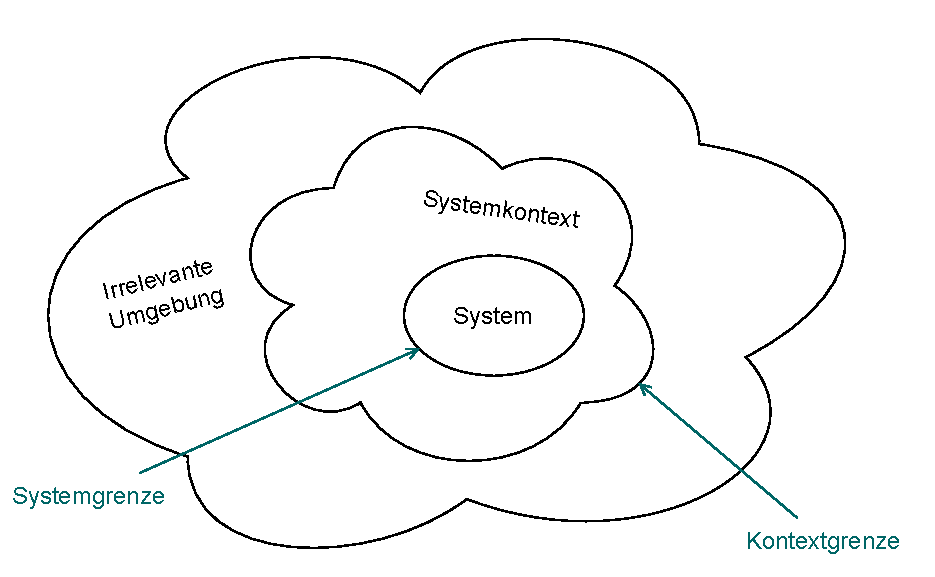
\includegraphics[scale=0.75]{Bilder/Kapitel-6/system-system.pdf}
	\caption[System, Systemkontext und irrelevante Umgebung]{System, Systemkontext und irrelevante Umgebung. Eigene Abbildung in Anlehnung an \cite[15]{poh15}}
	\label{fig:system-system}
\end{figure}

\vspace{\baselineskip} %%% für Druck

Die Grenze zwischen dem Softwaresystem und dem Systemkontext bezeichnet man als Systemgrenze. Abbildung~\ref{fig:system-system} zeigt in der Mitte das System (das zu entwickelnde Softwareprodukt) und getrennt durch die Systemgrenze es umgebend seinen System\-kontext. Die Außengrenze des Systemkontexts bildet die sogenannte Kontextgrenze. Diese trennt die relevante Umgebung des Systems (den Systemkontext) von der irrelevanten Umgebung des Systems. Aspekte, die (von der Mitte aus gesehen) außerhalb der Kontextgrenze liegen, haben keinen Einfluss auf den Entwicklungsprozess des Softwaresystems. Insbesondere erzeugen sie keine Anforderungen an das System.

Die Bestimmung des Systemkontexts ist eine wichtige Aufgabe in einem Softwareentwicklungsprojekt. Ein fehlerhaft oder unvollständig festgelegter Systemkontext wird meist erst beim Betrieb des fertigen Softwareprodukts auffallen und sich zum Beispiel durch fehlende Schnittstellen zu anderen Systemen, unzureichende Unterstützung vorhandener Geschäftsprozesse oder Nichtberücksichtigung der Wünsche einzelner Nutzergruppen äußern. Ein ungünstig festgelegter Systemkontext kann sich im Übrigen nicht nur durch \textbf{fehlende} Aspekte äußern, sondern auch darin, dass das neue System in Kontexten agiert, die schon durch vorhandene Systeme abgedeckt werden können. In solchen Fällen sind Ressourcen des Softwareentwicklungsprojekts womöglich unnötig eingesetzt worden.

Der \marginline{Systemkontext und An\-for\-derungs\-ermitt\-lung} Zeitpunkt der Festlegung des Systemkontexts in einem Softwareentwicklungsprojekt ist abhängig von der Art des eingesetzten Vorgehensmodells. Sequentielle Modelle bestimmen den Systemkontext üblicherweise während des Teilprozesses der Anforderungsermittlung. Die Ermittlung konkreter Anforderungen und die Bestimmung des Systemkontexts sind dabei eng verbunden. Eine komplett lineare Abfolge zwischen Bestimmung des Systemkontexts und Bestimmung der Anforderungen ist nicht realistisch. Gerade zu Beginn der Requirements Engineering-Phase werden Grauzonen in der Abgrenzung zwischen System und Systemkontext auf der einen Seite, aber auch zwischen Systemkontext und irrelevanter Umgebung auf der anderen Seite bestehen. Mit Abschluss der Requirements Engineering-Phase ist grundsätzlich auch die Festlegung des Systemkontexts abgeschlossen. Sollte die Änderung von Anforderungen im Softwareentwicklungsprojekt nach der Requirements Engineering-Phase aber möglich sein, kann sich auch der Systemkontext noch verändern. Bei konfigurierbaren Systemen, die für die Bedürfnisse verschiedener Nutzergruppen unterschiedlich angepasst werden können, kann sich die Systemgrenze zwischen den einzelnen konfigurierten Produktversionen unterscheiden.

Agile Modelle verzichten komplett darauf, den Systemkontext schon zu Beginn des Softwareentwicklungsprojekts abschließend festzulegen. Hier können sich in Abhängigkeit der Veränderung von Anforderungen Systemgrenze und Kontextgrenze mit jeder Iteration verschieben.

\vspace{2mm} %%% für Druck

\minisec{Dokumentation des Systemkontexts}

Für die Darstellung des Systemkontexts werden unterschiedliche Notationen in der Literatur vorgeschlagen. \marginline{Kom\-po\-nen\-ten\-diagramm} Aus dem Umfeld der UML-Diagramme könnte man das Komponentendiagramm verwenden, das Komponenten und ihre Schnittstellen darstellen kann. Das zu entwickelnde System könnte als eine Komponente und jedes Element des Systemkontexts als weitere Komponente modelliert werden. Der hauptsächliche Einsatzzweck eines UML-Komponentendiagramms ist allerdings die Modellierung von Softwarearchitekturen. Es wird üblicherweise im Prozess des Softwareentwurfs eingesetzt, um die Komponenten des zu entwickelnden Software\-systems und ihre Schnittstellen untereinander darzustellen. Insofern ist das Komponentendiagramm auf eine deutlich niedrigere Abstraktionsebene optimiert, als sie für die Darstellung des Systemkontexts benötigt wird und legt gleichzeitig den Fokus auf systeminterne Beziehungen anstatt auf die Beziehungen des Systems mit seiner 
\linebreak %%% für Druck
Umgebung.

Beziehungen des Systems mit seiner Außenwelt modelliert das UML-Anwen\-dungs\-fall\-diagramm, das daher auch ein potentieller Kandidat für die Darstellung des System\-kontexts ist. \marginline{An\-wen\-dungs\-fall\-diagramm} Es beschreibt, welche Anwendungsfälle mit dem System durchgeführt werden können, aber nicht auf welche Weise das System diese realisiert. Insofern bietet das Anwendungsfalldiagramm im Unterschied zum Komponenten\-diagramm das für die Darstellung des Systemkontexts gewünschte hohe Abstraktions\-niveau. Gleichzeitig ist die Syntax des UML-Anwendungsfalldiagramms auch für 
\linebreak %%% für Druck
IT-ferne Personen leicht erlernbar, sodass Anwendungsfalldiagramme sehr gut in Diskussionszusammenhängen mit den Kunden eingesetzt werden können. Zudem werden Anwendungsfalldiagramme häufig sowieso an anderer Stelle des Requirements Engineering eingesetzt. Genau dies spricht aber auch gegen das Anwendungsfall\-diagramm für die Darstellung des Systemkontexts, denn auch das Anwendungsfalldiagramm hat eigentlich andere Einsatzgebiete. In erster Linie wird ein Anwendungs\-fall\-diagramm verwendet, um auf einem sehr hohen Abstraktionsniveau die Interaktion der verschiedenen (menschlichen und nicht-menschlichen) Nutzergruppen mit dem System zu modellieren und ist damit ein Diagramm zur Darstellung von Verhalten. Die Verwendung eines Verhaltensdiagramms zur Darstellung des System\-kontexts, bei der man einen strukturellen Fokus einnimmt, ist nicht optimal.

\begin{figure}[h!]
	\centering
	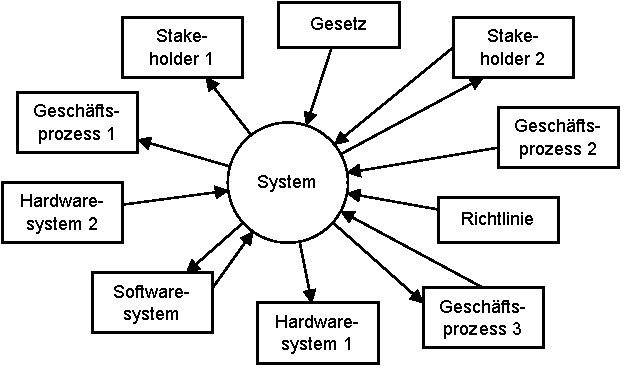
\includegraphics[scale=1.0]{Bilder/Kapitel-6/system.pdf}
	\caption{Kontextdiagramm der Strukturierten Analyse}
	\label{fig:kontextdiagramm_strukturierte_analyse}
\end{figure}

Außerhalb \marginline{Kontext\-diagramm} der Diagrammarten der UML existiert dagegen ein spezifisches Diagramm zur Darstellung des Systemkontexts, das sogenannte Kontextdiagramm der Strukturierten Analyse, die wir im historischen Überblick zur Entstehung des Software\-engineering in Abschnitt~1.1 kurz % TODO Referenz Abschnitt~\ref{sec:Kap-1.1}
angesprochen hatten. Als Bestandteil der Strukturierten Analyse gehört das Kontextdiagramm nicht zum Bereich der objektorientierten Softwareentwicklung, es ist nicht \textbf{Objekt}-orientiert, sondern \textbf{Datenfluss}-orientiert. Es wird, da es sehr bekannt ist -- aber sicher auch mangels anderer guter Alternativen -- auch in vielen objektorientierten Softwareentwicklungsprojekten eingesetzt. Abbildung~\ref{fig:kontextdiagramm_strukturierte_analyse} zeigt ein Kontextdiagramm.

Das System wird in der Mitte des Diagramms als Kreis dargestellt und ist von den Elementen des Systemkontexts (dargestellt als Rechtecke) umgeben. Die Pfeile zwischen dem System und den Elementen des Systemkontexts zeigen Datenflüsse in und aus dem System und symbolisieren so die zukünftigen Schnittstellen zwischen dem System und seiner Umgebung. Durch die sehr überschaubare Menge an Syntax\-elementen ist das Kontextdiagramm wie das UML-Anwendungsfalldiagramm auch für technisch nicht-versierte Kunden leicht verständlich. Gerade zu Beginn der Require\-ments Engineering-Tätigkeiten reicht es häufig, darzustellen, an welchen Stellen Schnittstellen zwischen dem zu entwickelnden System und dem System\-kontext berücksichtigt werden müssen, und nicht anzugeben, welche Informationen genau über diese Schnittstellen ausgetauscht werden sollen. Wie in Abbildung~\ref{fig:kontextdiagramm_strukturierte_analyse} sind dann die Pfeile nicht beschriftet und die Datenflüsse somit nicht näher spezifiziert. Bei konkreteren Beschreibungen des Systemkontexts und der Datenflüsse sollte man darauf achten, die Informationen, die zwischen dem System und Elementen des Systemkontexts ausgetauscht werden, nicht zu detailliert und nicht zu technisch darzustellen, um die einfache Lesbarkeit des Diagramms auch für die Kunden beizubehalten. 

\begin{itemize}[
	label={\sttpHervorhebung{$\Rightarrow$}},
	]
	\item Das UML-Komponentendiagramm sollte man eher nicht für die Darstellung des Systemkontexts verwenden. Das UML-Anwendungsfalldiagramm ist die geeignetste Diagrammart, wenn man das UML-Umfeld nicht verlassen möchte. Das Kontextdiagramm der Strukturierten Analyse kann man aufgrund seiner Einfachheit auch ohne Kenntnis der Methode der Strukturierten Analyse gut einsetzen. Ansonsten bleibt natürlich immer auch die Möglichkeit, sich mit einfachen Kästen und Pfeilen ein projektspezifisches Kontextdiagramm zu erstellen.
\end{itemize}
\subsubsection{Produktumfang}
\label{sec:Kap-6.1.3.2}

Die Wahl der Systemgrenze bestimmt, welche Aufgabenbereiche das zu entwickelnde System im späteren Einsatz abdecken muss und welche Aufgaben außerhalb des zu entwickelnden Systems liegen und daher von anderen Systemen, von Prozessen oder Personen geleistet werden müssen. Die Aufgabenbereiche des zu entwickelnden Systems bilden den sogenannten Produktumfang (engl. scope) des Systems. Insofern sind die Bestimmung des Systemkontexts und die Festlegung des Produktumfangs eng verbunden. Es geht bei der Festlegung des Produktumfangs um die Abgrenzung zwischen dem, was das Softwareprodukt leisten soll und dem, was außerhalb seines Aufgabenbereichs liegt.

\begin{figure}[h!]
	\centering
	\vspace{2mm} %%% für Druck
	\vspace{\baselineskip} %%% für Druck
	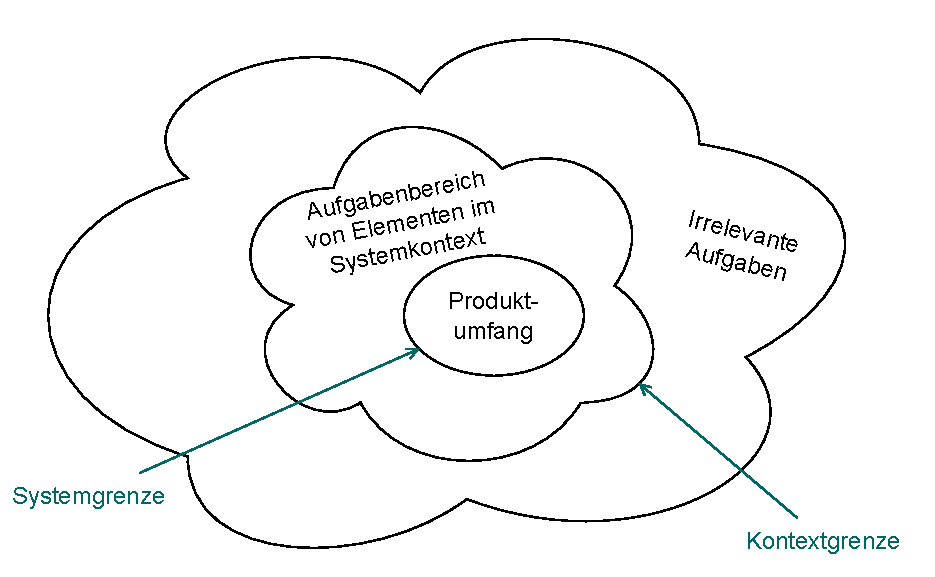
\includegraphics[scale=0.75]{Bilder/Kapitel-6/system-produktumfang.pdf}
	\caption{Aufgabenteilung zwischen dem System und seiner Umgebung}
	\label{fig:system-produktumfang}
	\vspace{\baselineskip} %%% für Druck
\end{figure}

Abbildung~\ref{fig:system-produktumfang} zeigt wieder den Zusammenhang zwischen dem zukünftigen Softwaresystem, seinem Systemkontext und der irrelevanten Umgebung. Diesmal jedoch nicht wie in Abbildung~\ref{fig:system-system} aus einer strukturellen Sicht, sondern aus dem Blickwinkel der Aufgabenverteilung im Betrieb des Softwaresystems. Beschneidet man -- bei gegebener Menge an durchzuführenden Aufgaben -- den Produktumfang des zukünftigen Systems, müssen Elemente des Systemkontexts zusätzliche Aufgaben übernehmen, und umgekehrt. Verschiebt man die Kontextgrenze nach außen, bekommen irrelevante Aufgaben eine Relevanz und müssen von Elementen des Systemkontexts übernommen werden, und umgekehrt.

Der englische Begriff \textit{Scope} für den Produktumfang hat sich im Gegensatz zu den englischen Begriffen Requirements Engineering und Stakeholder in der deutschsprachigen Literatur (noch) nicht durchgesetzt. Wir bleiben daher bei der deutschen Übersetzung, auch wenn der englische Begriff das Konzept besser beschreibt:

\vspace{2mm} %%% für Druck

\begin{itemize}[
	label={\sttpHervorhebung{$\Rightarrow$}},
	]
	\item Das englische Scope kann man außer mit Umfang auch mit Raum, Bereich oder Aufgabenbereich übersetzen. Und die Beschreibung des Produktumfangs besteht eben nicht aus einer Liste der Funktionalitäten des Softwareprodukts, sondern auf einer abstrakteren Ebene aus der Angabe der Aufgabenbereiche, für die das Softwareprodukt zuständig sein soll. Zur Verdeutlichung eine Analogie aus dem Personalverwaltungsbereich: Der Produktumfang entspricht eher einer Arbeitsplatzbeschreibung statt einer Liste der konkreten Arbeits\-tätig\-keiten eines Mitarbeiters.
\end{itemize}

\vspace{2mm} %%% für Druck

Ausgehend vom festgelegten Produktumfang werden konkrete Anforderungen an das zu entwickelnde Softwareprodukt ermittelt. Um hier Ressourcen nicht unnötig zu investieren, sollten die Aufgabenbereiche, die man dem Produktumfang zuordnet, gut durchdacht sein. Das beinhaltet auch die Überlegung, ob sehr verschiedenartige Aufgabenbereiche einfach durch verschiedene Komponenten des späteren Softwaresystems abgedeckt werden oder ob es mehrere eigenständige Produkte geben soll. Im Zoo-Beispiel entwirft Frau Dr. Walther mit ihren ersten vagen Vorstellungen ein Softwareprodukt, das vielfältige Informationen zu den Zootieren bereitstellt, den Besuchern erlaubt, an der Namensgebung der Tiere mitzuwirken, die Übernahme von Tierpatenschaften ermöglicht, die Arbeitsabläufe der Tierpfleger inklusive der Futter\-bestellung verwaltet, die Ausleihe von Tieren und Käfigen aus anderen Zoos unterstützt, die Terminverwaltung der Tierärzte übernimmt und Eintrittskarten für den Zoo verkauft. Bevor man hier den sehr aufwändigen Prozess der Anforderungs\-ermittlung startet, sollte man sich zunächst mit den Stakeholdern darüber verständigen, ob ein einziges Softwareprodukt diese vielen verschiedenen Aufgabenbereiche übernehmen soll oder ob sie Bestandteil unterschiedlicher Software\-entwicklungs\-projekte -- nacheinander oder parallel stattfindend -- sein sollen.

In Softwareentwicklungsprojekten, die nach sequentiellem Vorgehen arbeiten, wird der Produktumfang oft vom Auftraggeber schon vor Start des Softwareentwicklungsprojekts vorgegeben. Der Produktumfang -- und seine Ausdifferenzierung in konkrete Anforderungen -- ist oft auch schon Grundlage des Vertrags zwischen Auftraggeber und Auftragnehmer und im Rahmen des weiteren Softwareentwicklungsprojekts damit nicht mehr grundlegend veränderbar. In agilen Projekten finden durch die stetige Änderungsmöglichkeit im Bereich der Anforderungen automatisch kontinuierliche Verhandlungen zwischen Auftraggeber und Auftragnehmer über den Produkt\-umfang statt. Manche agile Modelle, wie zum Beispiel Extreme Programming, stellen die Notwendigkeit der expliziten Bestimmung des Produktumfangs sogar grundsätzlich in Frage.

\minisec{Rahmenbedingungen}

An dieser Stelle möchten wir noch kurz auf die schon im Kapitel zu Vision und Zielen angesprochenen Rahmenbedingungen zurückkommen. Wir hatten dort zwischen Rahmenbedingungen unterschieden, die in Zusammenhang mit dem Software\-produkt stehen und solchen, die sich auf das Entwicklungsprojekt beziehen. Die produkt\-bezogenen Rahmenbedingungen, wie Gesetze und Richtlinien, die das Softwareprodukt im Betrieb einhalten muss oder die die Architektur des zu entwickelnden Produkts bestimmen, aber auch vorgegebene Hardwareumgebungen für den Betrieb des Systems, sind Elemente des Systemkontexts. Sie werden bei einer systematischen Beschäftigung mit dem Systemkontext während des Entwicklungsprojekts mit berücksichtigt und würden so ihren Weg auch in die Anforderungen finden. Projektbezogene Rahmenbedingungen, wie Zeit- und Kostenbudgets, die zeitliche Verfügbarkeit von Mitarbeitern, die Qualifikation der Mitarbeiter oder auch Möglichkeiten bzw. Unmöglichkeiten Mitarbeiter während des Projekts zu bestimmten Themen fortzubilden, sind nicht Teil des Systemkontexts. Da sie aber entscheidend auf Produktumfang und Systemkontext einwirken können, dürfen sie nicht unberücksichtigt bleiben. Häufig werden sie daher den produktbezogenen Rahmenbedingungen gleichgestellt und als eine besondere Art von Anforderungen (die sogenannten Randbedingungen) behandelt. Wir vertiefen dieses Thema in Abschnitt~\ref{sec:Kap-6.2.2}.
\newpage
\cleardoublepage
\chapter*{Währenddessen im Zoo ~~~ \raisebox{-0.35cm}{
\includegraphics[height=1.0cm]{Bilder/elephant_emoji.png}}}
\addcontentsline{toc}{section}{Währenddessen im Zoo ~~~ \raisebox{-0.25cm}{
\includegraphics[height=0.8cm]{Bilder/elephant_emoji.png}}}
\markboth{Währenddessen im Zoo ~ \raisebox{-0.15cm}{
\includegraphics[height=0.6cm]{Bilder/elephant_emoji.png}}}{\raisebox{-0.15cm}{
\includegraphics[height=0.6cm]{Bilder/elephant_emoji2.png}} ~ Währenddessen im Zoo}
\label{sec:Lektion-4-Zoo}

\marginline{~\\~\\Lektion~1, Seite~\pageref*{sec:Lektion-1-Zoo}\\~\\Lektion~2, Seite~\pageref*{sec:Lektion-2-Zoo}}
\sttpUniversalkasten{Was bisher geschah}{Der städtische Zoo ist an das Softwareunternehmen herangetreten, in dem Sie arbeiten, um zu eruieren, an welchen Stellen Zooabläufe mit Software unterstützt werden könnten und wie der öffentliche Zooauftritt insgesamt digitaler werden kann. Auf einem ersten Brainstorming-Workshop zwischen Softwareteam und Zooteam hat man sich auf die Durchführung eines Vorprojekts geeinigt, in dem der inhaltliche Rahmen für die zukünftige Zusammenarbeit fest\-gelegt werden soll. Erste Diskussionsergebnisse des Workshops zur Domäne Zoo, ihren Abläufen und Aufgaben sowie Überlegungen zum weiteren Vorgehen wurden festgehalten.}

\vspace{1em}


\sttpUniversalkasten{}{
\minisec{Was (ohne unsere Anwesenheit) noch passiert ist}
\vspace{1mm}
Mittlerweile wurden zwei Arbeitsgruppen gebildet. Die Arbeitsgruppe „Domänenmodellierung“ leitet Magnus Fryt, Requirement Engineer im Softwareunternehmen. Von Seiten des Softwareteams nimmt außerdem Paul Klipper (Software\-entwickler) teil, von Seiten des Zoos die beiden Tierpfleger:innen Ruth Temper und Adrian Droschke. Die Tierärztin des Zoos, Wiebke Mellier kann bei Bedarf hinzugeholt werden. Die Arbeitsgruppe „Entwicklungsplanung“ setzt sich zusammen aus Inga Schwab (Leiterin Vorprojekt) und Joris Jonson (Softwarearchitekt) sowie Frau Dr. Walther (Zoodirektorin), Lars Qwert (Marketingchef des Zoos) und Helmut Frohn (oberster Tierpfleger im Zoo). In beiden Arbeitsgruppen haben erste Treffen stattgefunden. \newline
In der AG Entwicklungsplanung hat man sich darauf verständigt, sich im aktuellen Vorprojekt nur ausgewählte Vorhaben der Zoowünsche detaillierter anzusehen, aber grundsätzlich an der Vision einer umfassenden Zoo-Ablaufautomatisierung und Zoo-Digitalisierung festzuhalten -- und dement\-sprechend zukünftiges Erweiterungspotenzial nie aus dem Blick zu verlieren.} 

\clearpage

\minisec{Treffen der Arbeitsgruppe Entwicklungsplanung}

Ausgehend von der von Frau Dr. Walther vorgenommenen Priorisierung der Zoo\-wünsche wird über das weitere Vorgehen diskutiert. 

\marginline{~\\~\\~\\Lektion~2, Seite~\pageref*{text:lektion2_whiteboard_s1}}
% Karteikarte Fallbeispiel Zoo

\sttpKarteikarte{12.5cm}{\sttpKarteikarteSkalierungsfaktor}{\sttpKarteikarteRotierungswinkel}{Überlegungen zum Produkt}%
	{Thema:}{Prioritäten}%
	{Details:}{Am wichtigsten: Umfangreiche Informationen auf der Website zu unseren Tieren und eine Softwareunterstützung beim Futterbestellprozess. \newline Zweite Priorität: die Einbindung der Besucher bei der Namensgebung neugeborener Tiere, ein automatisiertes Patenschaftssystem und der Online-Eintrittskartenverkauf. \newline Weitere Wünsche: Terminverwaltung Tierärzte, komfortableres System zur Tier- und Käfigausleihe.}%
	{Fr. Walther (Zoodirektorin)}
	
	
	


\textbf{Frau Walther:} „Recht dringend ist die Verbesserung des Tierfutter\-bestell\-prozesses. Der läuft aktuell komplett ohne spezialisierte Softwareunterstützung und sehr dezentral, das bindet extrem viel Personalressourcen auf allen Ebenen des Zoos und ist darüber hinaus sehr fehleranfällig. Zudem liegt uns sehr viel daran, in der Region sichtbarer zu werden und auch mehr Besucher:innen anzuziehen. Hierfür benötigen wir eine grundlegende Umgestaltung des digitalen Zoo-Auftritts, perspektivisch auch mit interaktiven Inhalten. Ich habe schon verstanden, dass wir unsere Wunschvorstellungen in diesem Bereich für eine erste Umsetzung noch deutlich eingrenzen müssen. Aber besser als jetzt wird es allemal gehen: Aktuell gibt es nur eine sehr basale Website mit Informationen zu Eintrittspreisen und Öffnungszeiten, noch nicht einmal eine Übersicht der Tierarten im Zoo.“ 

\textbf{Auszug aus dem anschließenden Protokoll:}
\begin{itemize}
	\item Im Fokus werden zwei Vorhaben stehen: 1. Der zukünftige digitale Zoo-Auftritt mit integriertem Tier-Informationssystem (Arbeitstitel: Zoo-Auftritt), 2. Die Begutachtung der aktuellen Zooprozesse im Bereich der Futterbestellung mit dem Ziel, Automatisierungspotenzial aufzuzeigen (Arbeitstitel: Futter-
	\linebreak %%% für Druck
	bestellung).
	\item Die gewünschte Einbindung der Zoobesucher bei der Namensgebung der Tiere soll im Rahmen des Tier-Informationssystems realisiert werden.
	\item Für den Online-Kartenverkauf soll ein auf dem Markt verfügbares konfigurierbares Standardsystem zum Einsatz kommen, das mit dem digitalen Zoo-Auftritt verbunden wird. Das Softwareteam wird den Zoo bei der Auswahl beraten.
	\item Ein automatisiertes Patenschaftssystem wird zunächst zurückgestellt, soll sich aber zukünftig an das Tier-Informationssystem anbinden lassen. Informationen zum Patenschaftssystem des Vogelparks Hohenhausen werden durch den Zoo eingeholt.
	\item Die Ablösung der seit vielen Jahren eingesetzten Softwarelösungen für die Käfig- und Tierausleihe sowie für die Terminverwaltung der Tierärzte wird aktuell nicht angegangen. Zwar gibt es Unzufriedenheiten mit den verfüg\-baren Funktionalitäten, doch sind zahlreiche Arbeitsprozesse mittlerweile an die Beschränkungen der Software angepasst worden, so dass kein prioritärer Handlungsbedarf besteht. 
\end{itemize}

\textbf{Frau Schwab:} „Lassen Sie uns für unsere zwei prioritären Vorhaben konkreter werden: Welche Ziele verfolgen wir?, welche Stakeholder müssen eingebunden werden? und so weiter. Beginnen wir heute noch mit dem Vorhaben Futterbestellung, das ist überschaubarer. Im morgigen Treffen reden wir dann über das Vorhaben Zoo-Auftritt. Zur Futterbestellung: Wir hatten uns ja schon darauf verständigt, dass wir von Seiten unseres Softwareunternehmens jetzt zunächst nur die aktuellen Futter\-bestell\-prozesse im Zoo analysieren, im Anschluss dann einen Vorschlag unterbreiten, an welchen Stellen wir inwiefern Potenzial von Softwareunterstützung sehen und dann nochmal mit der Zooleitung verhandeln, in welchem Umfang wir dieses Projekt in Richtung der Erstellung einer konkreten Anforderungsspezifikation weiterführen. Lassen Sie uns Vision und Ziele aber dennoch schon in Richtung dieser zukünftigen Futterbestellautomatisierung ausrichten und nicht nur auf die aktuell anstehenden Prozess-Begutachtungen.“

\vspace{\baselineskip}

\textbf{Diskussionsergebnisse „Automatisierung Futterbestellung“}

%\vspace{-0.5cm}
{ %% Scope beginnen (damit \renewcommand keine Auswirkung auf andere Karteikarten hat)
	\renewcommand{\sttpKarteikarteSkalierungsfaktor}{0.85}
	
	\begin{addmargin*}[0cm]{-\marginparwidth}
	\begin{addmargin*}[0cm]{-\marginparsep}

	\begin{center}
		\begin{tabular}{ p{8.2cm} p{8.2cm} }
		%\begin{tabular}{ | p{8.2cm} | p{8.2cm} | }
			\vspace{-0.5cm}
			\begin{center}
				\sttpKarteikarte{9.5cm}{\sttpKarteikarteSkalierungsfaktor}{\sttpKarteikarteRotierungswinkel}{Vision}%
{}{Die überwiegend manuell ablaufenden Prozesse der Futterbestellung werden durch eine softwaregestützte Automati\-sierungslösung ersetzt. Die Tierpfleger haben wieder mehr Freiraum für ihre Fachaufgaben in der Versorgung der Tiere. Fehlerhafte Futterbestellungen werden verhindert. Das Futterbestellsystem wird an die Einkaufs- und Abrechnungs\-systeme der Zooverwaltung angebunden.
\begin{flushright}
	 \textnormal{\textsf{\footnotesize{Version 1.0}}}
\end{flushright}
}%
{}{}% Text zum 2. Teil bleibt leer -> keine Anzeige
{}% Ersteller bleibt leer -> keine Anzeige
			\end{center}
	
			\vspace{-0.5cm}
			\begin{center}
				\sttpKarteikarte{9.5cm}{\sttpKarteikarteSkalierungsfaktor}{\sttpKarteikarteRotierungswinkel}{Stakeholder}%
{}{Tierpfleger, Lagerverwalter, Rechnungsabteilung der Zooverwaltung, IT-Abteilung des Zoos, ggf. weitere Abteilungen der Zooverwaltung, ggf. Futterlieferanten}%
{Anmerkungen:}{Sollten sich die Bestellprozesse für verschiedene Tierarten sehr unterscheiden, müssen unbedingt Tierpfleger aus verschiedenen Gebieten einbezogen werden.
\begin{flushright}
	\textnormal{\textsf{\footnotesize{Version 1.0}}}
\end{flushright}
}
{}% Ersteller bleibt leer -> keine Anzeige
			\end{center}
			&
			\vspace{-0.5cm}
			\begin{center}
				\sttpKarteikarte{9.5cm}{\sttpKarteikarteSkalierungsfaktor}{\sttpKarteikarteRotierungswinkel}{Ziele}%
{}{Die Tierpfleger von verwaltungstechnischen Aufgaben befreien \newline 
	Den Futterbestellprozess beschleunigen \newline 
	Den Futterbestellprozess zentralisieren \newline 
	Überblick über den Futterlagerbestand besitzen \newline 
	Minimierung der Futterentsorgung aufgrund über\-schrittener Haltbarkeiten
\begin{flushright}
	\textnormal{\textsf{\footnotesize{Version 1.0}}}
\end{flushright}
}%
{}{}% Text zum 2. Teil bleibt leer -> keine Anzeige
{}% Ersteller bleibt leer -> keine Anzeige



			\end{center}
			\\
		\end{tabular}
	\end{center}

	\end{addmargin*}
	\end{addmargin*}
} %% Scope beenden (um \renewcommand lokal zu halten)

\clearpage

\minisec{Am nächsten Tag}

Auf der Agenda für heute steht das Vorhaben zum digitalen Zoo-Auftritt. Auch hier wird über Vision, Ziele, Stakeholder diskutiert. Die Marketingabteilung des Zoos hat im Vorfeld der Besprechung bei den Kolleg:innen schon Ideen gesammelt (s.~Abb.~\ref{fig:sprechblasen_ideen}), das Softwareteam sich anhand der bisherigen Diskussionen schon mal Gedanken zum Produktumfang und zu Schnittstellen des Systemkontexts gemacht. Man diskutiert und systematisiert.

\begin{figure}[h!]
	\centering
	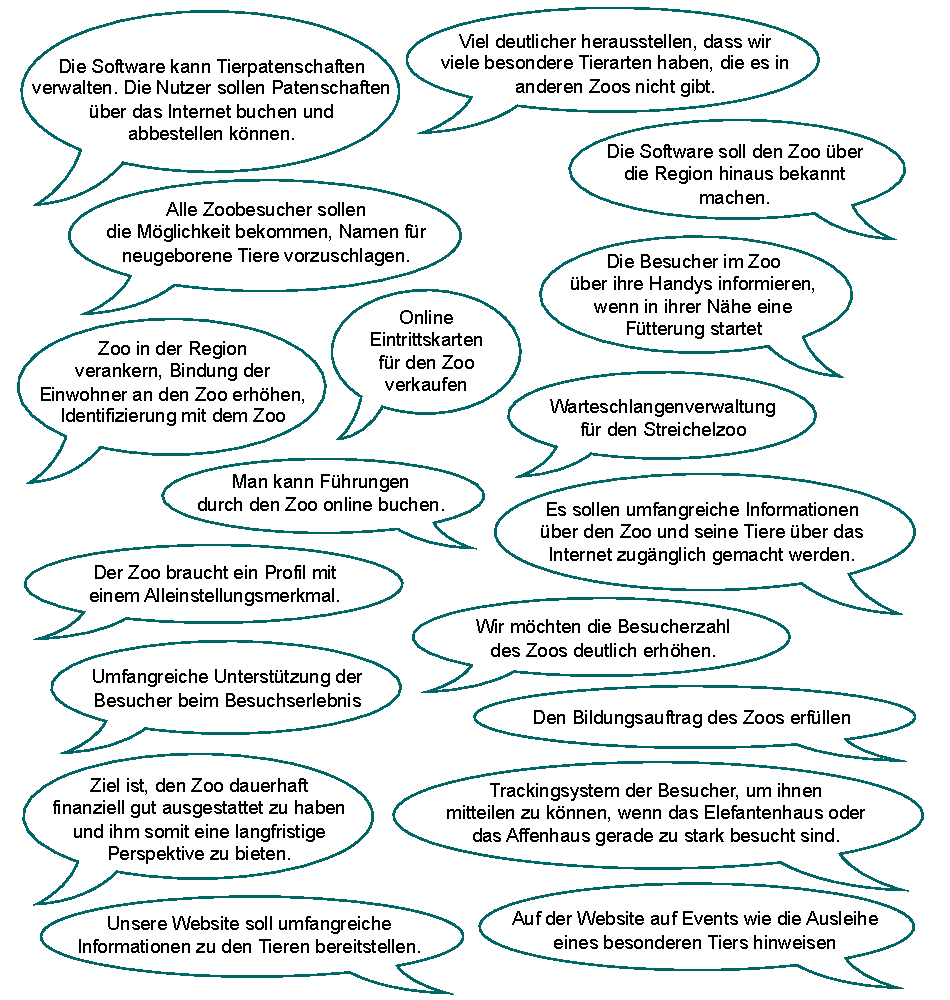
\includegraphics[width=\textwidth]{Bilder/Kapitel-6/sprechblasen_ideen.pdf}
	\caption[Zoo-Ideen zu Motivation, Zielen, Anforderungen etc.]{Unsystematische Mischung von Ideen zu Motivation, Zielen, Anforderungen, \ldots}
	\label{fig:sprechblasen_ideen}
\end{figure}

\clearpage

\minisec{Diskussionsergebnisse „digitaler Zooauftritt“}

{ %% Scope beginnen (damit \renewcommand keine Auswirkung auf andere Karteikarten hat)
	\renewcommand{\sttpKarteikarteSkalierungsfaktor}{0.85}

	\begin{addmargin*}[0cm]{-\marginparwidth}
	\begin{addmargin*}[0cm]{-\marginparsep}
	
	\begin{center}
		\begin{tabular}{ p{8.2cm} p{8.2cm} }
		%\begin{tabular}{ | p{8.2cm} | p{8.2cm} | }
			\vspace{-0.5cm}
			\begin{center}
				\sttpKarteikarte{9.5cm}{\sttpKarteikarteSkalierungsfaktor}{\sttpKarteikarteRotierungswinkel}{Motivation}%
{}{Zoobesuchern ein umfassendes Besuchserlebnis bieten \newline Zoo in der Region verankern und über die Region hinaus bekannt machen \newline Starke Identifikation der Einwohner mit dem Zoo schaffen \newline Den Bildungsauftrag des Zoos erfüllen.}%
{}{}% Text zum 2. Teil bleibt leer -> keine Anzeige
{}% Ersteller bleibt leer -> keine Anzeige
			\end{center}
			&
			\vspace{-0.7cm}
			\begin{center}
				\sttpKarteikarte{9.5cm}{\sttpKarteikarteSkalierungsfaktor}{\sttpKarteikarteRotierungswinkel}{Ziele}%
{}{Alleinstellungsmerkmale des Zoos bekannt machen \newline Steigende Besucherzahlen \newline Zusätzliche Kooperationspartner gewinnen (Studien\-gänge, Schulen, Kindergärten, Bildungsprojekte) und Koopera\-tions\-projekte akquirieren
\begin{flushright}
	\textnormal{\textsf{\footnotesize{Version 1.0}}}
\end{flushright}
}%
{}{}% Text zum 2. Teil bleibt leer -> keine Anzeige
{}% Ersteller bleibt leer -> keine Anzeige
			\end{center}
			\\
			\vspace{-0.5cm}
			\begin{center}
				\sttpKarteikarte{9.5cm}{\sttpKarteikarteSkalierungsfaktor}{\sttpKarteikarteRotierungswinkel}{Produktumfang und Schnittstellen}%
{Produktumfang}{klassische Website-Informationen (Öffnungszeiten, Preise etc.) \newline 
	basales Tier-Informationssystem \newline 
	Komponente zum Tiernamen-Voting \newline 
	spätere Erweiterungen: Auslastungsanzeigen der Zoo\-bereiche (Affenhaus etc.), Event-Benachrichtigungen für Zoo\-besucher
}%
{Schnittstellen}{Anbindung zum detaillierten Tier-Informationssystem der Universität \newline 
	Anbindung an Online-Kartenverkauf \newline 
	zukünftig: Anbindung an Patenschaftssystem, Anbindung an Buchungssystem für Zooführungen
\begin{flushright}
	\textnormal{\textsf{\footnotesize{Version 1.0}}}
\end{flushright}
}
{}{}% Text zum 2. Teil bleibt leer -> keine Anzeige
{}% Ersteller bleibt leer -> keine Anzeige
			\end{center}
			&
			\vspace{-0.5cm}
			\begin{center}
				\sttpKarteikarte{9.5cm}{\sttpKarteikarteSkalierungsfaktor}{\sttpKarteikarteRotierungswinkel}{Stakeholder}%
{}{Marketing-Abteilung, IT-Abteilung, Tierpfleger, Zoo\-besucher, verschiedene Abteilungen der Zooverwaltung, ggf. Zoologie-Studiengang der Universität
\begin{flushright}
	\textnormal{\textsf{\footnotesize{Version 1.0}}}
\end{flushright}
}%
{}{}% Text zum 2. Teil bleibt leer -> keine Anzeige
{}% Ersteller bleibt leer -> keine Anzeige
			\end{center}
			\\
		\end{tabular}
	\end{center}

	\end{addmargin*}
	\end{addmargin*}
} %% Scope beenden (um \renewcommand lokal zu halten)

\textbf{Frau Schwab:} „Der nächste Schritt in beiden Vorhaben ist jetzt die jeweils vorgesehenen Stakeholder zu kontaktieren und mit ihnen weiter an Visionen, Zielen, Produkt\-umfang und so weiter zu arbeiten und dann mit der Anforderungs\-sammlung zu beginnen. Das Vorhaben Futterbestellung geben wir am besten in die Hand der AG Domänenmodellierung, hier müssen ja jetzt hauptsächlich die Prozesse der \mbox{Domäne} diskutiert und dokumentiert werden. Unsere eigene AG Entwicklungs\-planung überführen wir in eine AG Zoo-Auftritt und kümmern uns um dieses Vorhaben.“
% 6.2
\clearpage
% ACHTUNG: im nächsten Abschnitt explizit mit "\markboth" die Texte für die Kopfzeilen neu setzen, da diese nach "Zoo" kaputt sind.
\section{Anforderungen}
\markboth{\thechapter~Requirements Engineering}{\thesection~Anforderungen}% Muss explizit gesetzt werden, da nach Kapitel Zoo kaputt.
\label{sec:Kap-6.2}

Das "`Software and Systems Engineering Vocabulary"' (SEVOCAB; siehe Kap.~1.1) % TODO Kap.~\ref{sec:Kap-1.1}
definiert den Begriff Anforderung (engl. requirement) aus verschiedenen Blick-
\linebreak %%% für Druck
winkeln. Aus der Perspektive eines Nutzers -- womit sowohl menschliche Nutzer als auch andere Softwareprodukte gemeint sind -- eines (zukünftigen) Softwareprodukts ist eine Anforderung ein

\sttpzitat{"`statement that translates or expresses a need and its associated constraints and conditions"'.}{\url{https://www.computer.org/sevocab}; Eintrag: requirement (1)}

\vspace{3mm} %%% für Druck

Aus den Bedürfnissen (need) der Nutzer ergeben sich -- sofern sie berücksichtigt werden -- die Funktionalitäten und Eigenschaften des zu entwickelnden Software\-produkts.

SEVOCAB, das Begriffsdefinitionen aus unterschiedlichen Standards gleichwertig nebeneinander stellt, führt für den Begriff requirement noch eine zweite Defini\-tion aus einem Standard zur Qualitätssicherung von Software auf. Danach ist eine Anforderung eine

\sttpzitat{"`condition or capability that must be met or possessed by a system, system component, product, or service to satisfy an agreement, standard, specification, or other formally imposed documents"'.}{\url{https://www.computer.org/sevocab}; Eintrag: requirement (2)}

\vspace{3mm} %%% für Druck

Hier wird der Begriff Anforderung aus Perspektive des zu erstellenden Softwareprodukts definiert. Danach beschreiben Anforderungen, welche Bedingungen oder Fähigkeiten ein System aufweisen bzw. erfüllen muss, um vorliegenden formellen Dokumenten (wie einem Vertrag oder einer Spezifikation) gerecht zu werden. Auf die Unterscheidung zwischen sogenannten Nutzeranforderungen und Systemanforderungen kommen wir in Abschnitt~\ref{sec:Kap-6.2.1} zurück.

\vspace{2mm} %%% für Druck

\minisec{Anforderungsquellen}

Anforderungen an ein zu erstellendes Softwareprodukt können aus unterschiedlichen Quellen stammen. Eine wichtige Kategorie von Quellen sind verschiedene Arten von Dokumenten, wie zum Beispiel Unternehmenshandbücher, die Organisations- und Arbeitsprozesse spezifizieren, die die zu erstellende Software abbilden bzw. unter\-stützen soll. Eine andere Kategorie von Anforderungsquellen sind existierende Softwareprodukte, deren Funktionalitäten in einer aktualisierten Version verbessert werden sollen bzw. Konkurrenzprodukte, deren Funktionalitäten auch im eigenen Softwareprodukt zur Verfügung stehen sollen. Auch Schnittstellenbeschreibungen benachbarter Softwareprodukte können Anforderungen enthalten bzw. generieren. Eine sehr wichtige Quelle von Anforderungen sind zudem Domänenmodelle. Letztendlich sind die Quellen von Anforderungen aber immer die Stakeholder. Und zwar zum einen, weil sie entscheiden, welche der anderen Quellen überhaupt Infor\-mations\-grundlage für die Anforderungsermittlung sein sollen. Zum zweiten und vielleicht auch vor allem, weil sie Bedürfnisse haben, die als Anforderungen an das Softwareprodukt formuliert werden müssen und die sich größtenteils nicht aus anderen (nichtmenschlichen) Quellen extrahieren lassen.
\subsection{Nutzeranforderungen und Systemanforderungen}
\label{sec:Kap-6.2.1}

Abbildung~\ref{fig:nutzer-vs-system} zeigt die Einteilung von Anforderungen in Nutzeranforderungen, System\-anforderungen und domänenbasierte Anforderungen. Hierbei handelt es sich um eine Kategorisierung anhand unterschiedlicher Blickwinkel. Nutzeranforderungen fokussieren den Blickwinkel "`Was möchten Nutzer (und Auftraggeber) tun bzw. vorfinden?"'. Systemanforderungen beschreiben "`Was muss das System dafür können bzw. gewährleisten?"'. Und domänenbasierte Anforderungen berücksichtigen die Ebene "`Welche (zusätzlichen) Anforderungen liefert die Domäne?"'.

\vspace{\baselineskip} %%% für Druck
\vspace{\baselineskip} %%% für Druck

\begin{figure}[h!]
	\centering
	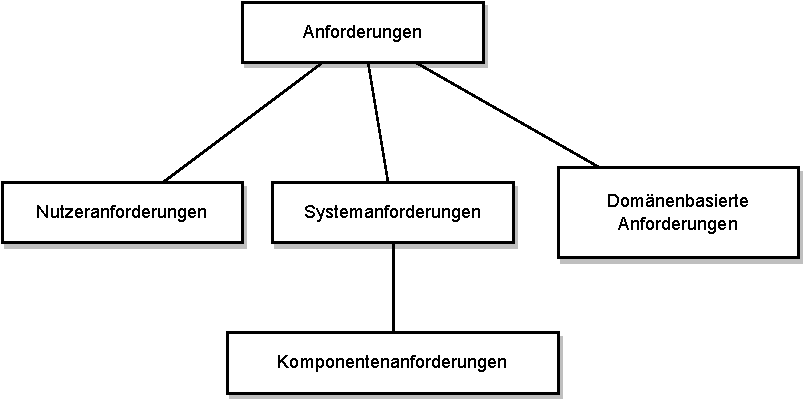
\includegraphics{Bilder/Kapitel-6/nutzer_vs_system.pdf}
	\caption{Nutzer-, System- und domänenbasierte Anforderungen}
	\label{fig:nutzer-vs-system}
\end{figure}

\vspace{\baselineskip} %%% für Druck

\minisec{Nutzeranforderungen}

Nutzeranforderungen sind Anforderungen, die aus Sicht und in der (Domänen)
\linebreak %%% für Druck
Sprache der Kunden formuliert sind. Sie sind die Form, in der Kunden ihre Bedürfnisse kommunizieren. Den größten Anteil an den Nutzeranforderungen haben Anforderungen, die das extern sichtbare Verhalten des Softwaresystems betreffen. Sie beschreiben, was ein Nutzer mit der Software tun will: welche Aktionen er ausführen können möchte und welche Ergebnisse er dabei erwartet. Aber auch Anforderungen, die das äußere Erscheinungsbild des Softwareprodukts betreffen (wie die Berücksichtigung des Coporate Design des Auftraggeber-Unternehmens oder die Gestaltung von Benutzeroberflächen), Anforderungen des Kunden an Qualitätsmerkmale des Produkts (\zb einfache Bedienbarkeit, schnelle Erlernbarkeit, das Vorhandensein kontextsensitiver Hilfe etc.) oder Kundenwünsche nach Schnittstellen zu Hard- und Softwaresystemen des Systemkontexts gehören zu den Nutzeranforderungen. Nutzeranforderungen sollten immer von einem zu erreichenden Ziel bzw. einem zu lösenden Problem der Stakeholder ausgehen: Eine Anforderung, für die selbst der Anforderungssteller nicht begründen kann, welchen Zweck sie erfüllt, wird in der Regel zu nicht genutzten Funktionalitäten oder unnötigen Eigenschaften des Softwareprodukts führen und dabei Entwicklungsressourcen verschwenden.

\vspace{2mm} %%% für Druck

\sttpseitenrandzitat{"`If your software does not have to satisfy a need, then you can build anything. However, if it is meant to satisfy a need, then you have to know what need is to build the right software"'}{\cite[3]{rob13}}

\vspace{2mm} %%% für Druck


Nutzeranforderungen können unterschiedlich stark ausdifferenziert sein. Eine recht abstrakte Nutzeranforderung auf einer hohen Ebene aus dem Zookontext könnte lauten:

\vspace{2mm} %%% für Druck

\sttpAnforderungText{Potentielle Zoobesucher sollen im Internet über neugeborene Tiere informiert werden.}

\vspace{\baselineskip} %%% für Druck

Ein zu erreichendes Ziel hinter dieser Anforderung könnte -- unter der Annahme, dass Babytiere Besuchermagneten sind -- die Erhöhung des Besucheraufkommens des Zoos sein. Die Anforderung ist aber so allgemein gehalten, dass man nicht bestimmen kann, welche Funktionalität der zukünftigen Software der Anforderungssteller genau einfordert. Eine detailliertere Nutzeranforderung aus dem gleichen 
\linebreak %%% für Druck
Kontext wäre:

\vspace{2mm} %%% für Druck

\sttpAnforderungText{Tierpfleger sollen die Namen neugeborener Tiere angeben können, um diese auf der Zoo-Website anzeigen zu können.}

\vspace{\baselineskip} %%% für Druck

Oder als sogenannte User Story formuliert, wie es vor allem in agilen Entwicklungsprojekten praktiziert wird:

\vspace{2mm} %%% für Druck

\sttpAnforderungText{Als Tierpfleger möchte ich den Namen eines neugeborenen Tiers angeben können, um diesen auf der Zoo-Website anzeigen zu lassen.}

\pagebreak %%% für Druck

\minisec{Systemanforderungen}

Aus einer solchen Nutzeranforderung ergeben sich Anforderungen an die Dienste des zukünftigen Softwareprodukts. Also: welche Bedingungen muss die Software \mbox{gewährleisten} bzw. welche Fähigkeiten muss sie besitzen, um die Nutzeranforderung erfüllen zu können. Im Beispiel muss sie die Möglichkeit bieten, die Namen der Tiere (irgendwie) zu erfassen, sie speichern, auf die gespeicherten Informationen zugreifen können und diese anzeigen können. Eine entsprechende Anforderung könnte lauten:

\vspace{2mm} %%% für Druck

\sttpAnforderungText{Die Software soll die Namen neugeborener Tiere erfassen, speichern und anzeigen.}

\vspace{\baselineskip} %%% für Druck

Eine solche, durch Verfeinerung einer Nutzeranforderung entstandene Anforderung nennt man eine Systemanforderung. Systemanforderungen beschreiben, welche
\linebreak %%% für Druck
Eigenschaften und Funktionalitäten die zukünftige Software aufweisen soll, um die in den Nutzeranforderungen ausgedrückten Bedürfnisse der Nutzer umsetzen zu können. Sie werden auf Grundlage der Nutzeranforderungen in Zusammenarbeit zwischen Kunden und Softwareentwicklungsteam erstellt. Wie Nutzeranforderungen können Systemanforderungen einen unterschiedlichen Detaillierungsgrad aufweisen. Die Systemanforderung könnte in einer konkreteren Form auch lauten:

\vspace{2mm} %%% für Druck

\sttpAnforderungText{Die Namen neugeborener Tiere sollen über Eingabemasken erfasst, in einer Datenbank gespeichert und als Liste angezeigt werden.}

\vspace{\baselineskip} %%% für Druck

Systemanforderungen sind weiterhin Anforderungen und keine Entwurfsbeschreibungen, welche erläutern, in welcher Weise Anforderungen im Softwaresystem umgesetzt werden. Dementsprechend sollten sie noch weitgehend lösungsneutral formuliert werden. Ähnlich wie bei den Zielen (Kap.~\ref{sec:Kap-6.1.2.2}) können aber Nutzer\-bedürfnisse oder Rahmenbedingungen bestehen, die den möglichen Lösungsraum einschränken. So sollte im Beispiel von oben die Erfassung der Tiernamen über Eingabemasken durchaus schon in der Anforderung thematisiert werden, wenn für den Kunden keine andere Art der Erfassung (\zb über das Hochladen von strukturierten Daten oder Dateien) in Frage kommt. Insgesamt ist die Grenze zwischen System\-anforderungen und Systembeschreibung fließend. Gerade bei sehr detailliert ausgearbeiteten Systemanforderungen ist man nicht mehr weit von einer Umsetzungs\-beschreibung entfernt. Der folgende Kasten zeigt an einem Beispiel den Unterschied zwischen einer Nutzeranforderung und einer Systemanforderung und vermittelt \mbox{Ihnen} zudem einen Eindruck von dem Unterschied zwischen Systemanforderung und Umsetzungsbeschreibung.

\pagebreak %%% für Druck

\sttpKasten{\textbf{Beispiel}
\\
\\
\underline{Nutzeranforderung:} Das System muss dem externen Abrechnungssystem der Tierärzte die notwendigen Informationen über die Behandlung der Zootiere zur Verfügung stellen können.
\\
\\
\underline{Systemanforderung:} Es muss eine Schnittstelle zwischen dem neuen Zooverwaltungssystem und dem von der Tierärztlichen Abrechnungsstelle betriebenen Abrechnungssystem eingerichtet werden. Über diese Schnittstelle müssen für jede Zootierbehandlung spätestens 2~Werktage nach der Behandlung folgende Informationen an das Abrechnungssystem übergeben werden: Name und Identifikationsnummer des Tierarztes, Identifikationsnummer des Zoos, \mbox{Name} und Art des Tiers, Art und Dauer der Behandlung, eingesetzte Medikamente.
\\
\\
\underline{Umsetzungsbeschreibung:} Das externe Abrechnungssystem bietet eine spezielle Webschnittstelle für Zoos an, über die Informationen in einem vorgegebenen JSON\footnote{JSON: JavaScript Object Notation. Ein Dateiformat in einer menschlich lesbaren Textform, welches zum Datenaustausch zwischen verschiedenen Anwendungen verwendet wird, s. \url{https://de.wikipedia.org/wiki/JavaScript_Object_Notation}}-Format an das Abrechnungssystem übertragen werden können. Das Zooverwaltungssystem wird diese Webschnittstelle nutzen, die in beiliegender Tabelle spezifizierten Informationen entsprechend ihres jeweiligen Datentyps in die benötigten Einträge des JSON-Formats transformieren und alle 48~Stunden automatisiert die jeweils neuen Datensätze übertragen. 
}

Eine \marginline{Kom\-po\-nen\-ten\-an\-for\-de\-run\-gen} eigene Unterkategorie von Systemanforderungen bilden die sogenannten Komponentenanforderungen. Diese legen den Blickwinkel auf eine konkrete Komponente des zukünftigen Systems und beschreiben, welchen Beitrag diese Komponente für bestimmte Systemanforderungen leisten soll. Die explizite Formulierung von Komponentenanforderungen spielt vor allem dann eine Rolle, wenn für ein zu entwickelndes Softwareprodukt vorhandene Komponenten genutzt bzw. von anderen Unternehmen zugeliefert werden sollen. Aus dem Blickwinkel des Herstellers der Komponente sind diese Komponentenanforderungen dann Nutzeranforderungen -- der Nutzer ist in diesem Fall das Softwareentwicklungsprojekt, das die Komponenten extern zukauft.

Die Aufteilung des Softwareprodukts in Komponenten und die entsprechende Ausdifferenzierung allgemeinerer Systemanforderungen in spezifischere Komponenten\-anforderungen beinhaltet natürlich schon Festlegungen im Bereich der System-
\linebreak
architektur und des Entwurfs des Softwareprodukts. Bei einer sehr strikten Auslegung der Trennung von Requirements Engineering-Tätigkeiten und Entwurfstätigkeiten würden Komponentenanforderungen daher erst ein Thema in der Phase des Entwurfs sein.

\minisec{Domänenbasierte Anforderungen}

Eine besondere Form von Anforderungen sind Anforderungen, die sich aus Domänen\-wissen ergeben (engl.: domain based requirement), welches nicht durch konkret formulierte Bedürfnisse der Nutzer abgedeckt ist. Wir behandeln domänenbasierte 
\linebreak %%% für Druck
Anforderungen als eigene Kategorie neben Nutzer- und Systemanforderungen, manche Autorinnen und Autoren führen sie als Unterkategorie von Nutzeranforderungen. Die Schwierigkeit für das Softwareentwicklungsteam bei Domänenwissen ist, dass es in der Regel nicht explizit vom Kunden in Anforderungen überführt wird. Ein Beispiel für domänenbasiertes Wissen im Zookontext wäre, dass Löwen niemals Teil des Streichelzoos sind. Für jeden, der mit der Domäne Zoo vertraut ist, ist das nicht erwähnenswert und findet seinen Weg daher in der Regel nicht in irgendwelche expliziten Nutzeranforderungen. Weiß man jedoch nicht, wie ein Streichelzoo funktioniert, entgehen einem unter Umständen wichtige Anforderungen, Restriktionen oder umgekehrt auch der Hinweis auf Aspekte, über die man sich keine weiteren Gedanken machen muss. Es ist daher für das Softwareentwicklungsteam sehr wichtig, sich nicht nur auf die vom Kunden explizit formulierten Nutzeranforderungen zu berufen, sondern sich Wissen über die Domäne anzueignen, zum Beispiel durch die, gemeinsam mit dem Kunden durchgeführte, Erarbeitung des Domänenmodells.

\minisec{Vorgehensmodelle und fließende Grenzen}

In Projekten, die nach klassischen Vorgehensmodellen arbeiten, sind Nutzeranforderungen üblicherweise Teil des Lastenhefts, während man die Verfeinerung in Systemanforderungen häufig erst im Pflichtenheft findet. In agilen Software\-entwicklungs\-projekten findet man eine Trennung in Lasten- und Pflichtenheft seltener und dem\-entsprechend eine stärkere Verbindung von Nutzer- und Systemanforderungen -- 
\linebreak %%% für Druck
üblicherweise auch ohne die \textbf{begriffliche} Trennung in Nutzer- und Systemanforderungen. Die notwendigen Arbeiten und der intensive Austausch mit den Kunden, um aus mitunter sehr grob formulierten Nutzeranforderungen spezifische System\-anforderungen zu extrahieren, bleiben aber auch in agilen Projekten nicht aus. In Projekten, die nach Scrum-Vorgaben arbeiten, passiert dies meist bei der Festlegung und Aufwandsschätzung der Anforderungen für den aktuellen Sprint. Unterschiede zwischen den Vorgehensmodellen ergeben sich zudem dadurch, dass in agilen Projekten das Softwareprodukt in der Regel schon während des laufenden Software\-entwicklungs\-projekts in der jeweils aktuellen Version produktiv eingesetzt wird. So wird auch in einigen agilen Vorgehensmodellen die Behebung von (von den Nutzern mitgeteilten) Fehlern in existierenden Funktionen der Software als gleichwertige Nutzeranforderung wie die Nutzeranforderung nach einer noch nicht implementierten Funktionalität angesehen.

Auch bei nicht-agilem Vorgehen ist die Trennung zwischen Nutzeranforderungen und Systemanforderungen letztendlich nur eine künstliche Kategorisierung, die zudem nicht immer trennscharf ist. Hier ein typisches Beispiel für eine Anforderung, die wie eine Systemanforderung aussieht, aber im konkreten Kontext eine Nutzer\-anforderung ist:

\sttpAnforderungText{Die Daten der Anwendung sollen in einer Postgres-Datenbank, Version 12 gespeichert werden.}

In vielen Softwareentwicklungsprojekten würde man eine solche Anforderung als Systemanforderung klassifizieren. Ein Kunde, der verschiedene Softwareprodukte einsetzt, die alle auf solch einer Postgres-Datenbank operieren, könnte diese Anforderung aber auch als Nutzeranforderung stellen, wenn es wichtig für ihn ist, dass auch das neue Softwareprodukt in die vorhandene Infrastruktur eingepasst werden kann. Die Einordnung einer Anforderung in die Kategorien Nutzer-, System- oder Komponentenanforderung ist also auch abhängig vom konkreten Softwareentwicklungsprojekt.
\subsection{funktionale und nichtfunktionale Anforderungen}
\label{sec:Kap-6.2.2}

Eine andere Form von Kategorisierung unterscheidet zwischen funktionalen und nichtfunktionalen Anforderungen. Diese Kategorisierung ist prinzipiell unabhängig von der zwischen Nutzer- und Systemanforderungen. So könnte man sowohl in funktionale Nutzeranforderungen und funktionale Systemanforderungen als auch in nichtfunktionale Nutzer- und Systemanforderungen trennen. Üblicherweise wird die so erzeugte Aufteilung in \textbf{vier} Kategorien aber weder in der Literatur explizit thematisiert, noch ist sie in der Praxis besonders bedeutsam. Je nach Kontext steht \textbf{entweder} die Trennung in Nutzer- und Systemanforderungen \textbf{oder} die Trennung in funktionale und nichtfunktionale Anforderungen im Vordergrund.

%hier gehört Abbildung "fig:funktionale_nichtfunktionale_anforderungen" eigentlich hin
\begin{figure}[h!]
	\begin{addmargin*}[0cm]{-\marginparwidth}
	\begin{addmargin*}[0cm]{-\marginparsep}
		\centering
		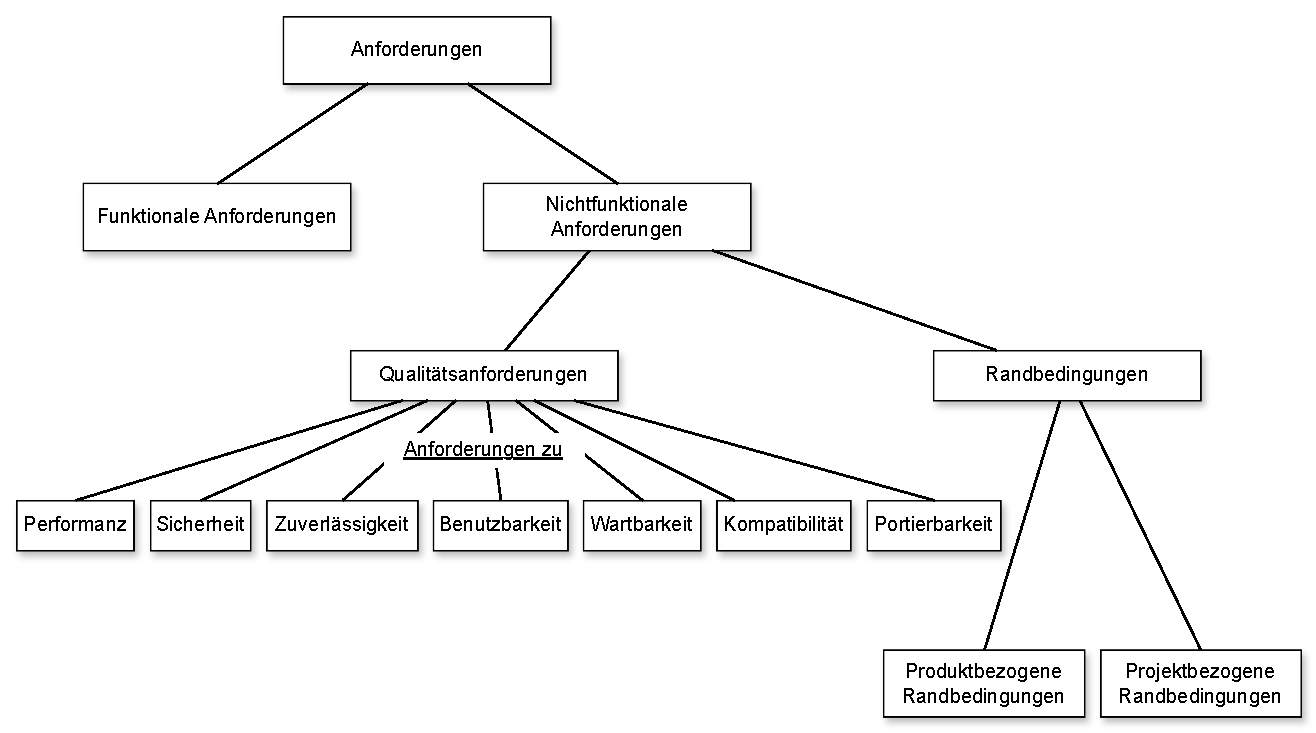
\includegraphics[scale=0.79]{Bilder/Kapitel-6/funktional.pdf}
		\caption{Funktionale und nichtfunktionale Anforderungen}
		\label{fig:funktionale_nichtfunktionale_anforderungen}
	\end{addmargin*}
	\end{addmargin*}
\end{figure}

Abbildung~\ref{fig:funktionale_nichtfunktionale_anforderungen} zeigt die Unterscheidung in funktionale und nichtfunktionale Anforderungen sowie die weitere Untergliederung der nichtfunktionalen Anforderungen. Man kann auch die funktionalen Anforderungen weiter untergliedern. In der Regel sind funktionale Anforderungen aber -- im Gegensatz zu großen Teilen der nichtfunktionalen Anforderungen -- so stark abhängig vom zu entwickelnden Softwareprodukt und dessen zu erwartenden Nutzergruppen, dass jede Form von allgemeiner Kategorisierung für den konkreten Softwareentwicklungsprozess wenig hilfreich ist.

\minisec{Funktionale Anforderungen}

Die funktionalen Anforderungen ergeben sich aus den Tätigkeiten, die Nutzer mit Hilfe des Softwareprodukts durchführen möchten. Sie beschreiben, welche Funktionalitäten (teilweise auch eingedeutscht Features genannt) das Softwareprodukt oder eines seiner Module bereitstellen soll, damit das Produkt von seinen Nutzergruppen sinnvoll eingesetzt werden kann. Funktionale Anforderungen beziehen sich somit auf das gewünschte Verhalten der Software. Sie können in sehr unterschiedlicher Form und auf unterschiedlichen Abstraktionsebenen auftreten. Funktionale Anforderungen sind zum Beispiel 

\begin{itemize}
	\item Vorgaben, welche Ausgabeparameter eine Funktion der Software bei gegebenen Eingabeparametern produzieren soll
	\item Beschreibungen, aus welchen Buttons und Menüeinträgen Benutzeroberflächen bestehen sollen
	\item Vorgaben, zu welchen externen Systemen Schnittstellen existieren müssen
\end{itemize}

Funktionale Anforderungen treten aber sehr häufig auch in der Form von Beschreibungen von Geschäftsprozessen und Anwendungsfällen auf, die durch die Software unterstützt oder durchgeführt werden sollen. Zudem kann über funktionale Anforderungen auch explizit spezifiziert werden, was die Software \textbf{nicht} tun soll.

\minisec{Nichtfunktionale Anforderungen}

Während funktionale Anforderungen festlegen, was das Softwareprodukt leisten können soll, bestimmen die nichtfunktionalen Anforderungen, in welcher Ausprägung, in welcher Qualität und unter welchen Umständen diese Leistungen erbracht werden sollen.

\vspace{\baselineskip} %%% für Druck

\sttpseitenrandzitat{"`Vereinfacht ausgedrückt, legen funktionale Anforderungen fest, was das Softwareprodukt tun soll, während die nichtfunktionalen Anforderungen spezifizieren, wie es arbeiten soll."'}{\cite[109]{bal09}}

\vspace{\baselineskip} %%% für Druck

Nichtfunktionale Anforderungen spezifizieren die Eigenschaften des Gesamtsystems oder schränken diese ein. In die Kategorie der nichtfunktionalen Anforderungen gehören damit Anforderungen, die übergreifende Eigenschaften, Leistungsmerkmale oder Restriktionen des Softwareprodukts betreffen, die nicht in \textbf{direktem} Zusammenhang zu einzelnen Funktionalitäten des Produkts stehen. Im Gegensatz zu den funktionalen Anforderungen, die sich meist einer oder wenigen Komponenten zuordnen lassen, kann die Umsetzung einer nichtfunktionalen Anforderung über viele verschiedene Komponenten des Softwareprodukts verteilt sein. Auch deswegen beeinflussen nichtfunktionale Anforderungen die zukünftige Architektur des Softwareprodukts in erheblichem Maße.

Nichtfunktionale Anforderungen werden heute meistens noch weiter unterteilt in die beiden Kategorien Qualitätsanforderungen und Randbedingungen. Die Randbedingungen nehmen dabei eine gewisse Sonderstellung innerhalb der nichtfunktionalen Anforderungen ein (\su). In mancher Literatur werden sie daher gar nicht den nichtfunktionalen Anforderungen zugeordnet, sondern bilden eine dritte Kategorie von Anforderungen neben den funktionalen und den nichtfunktionalen Anforderungen.

\minisec{Qualitätsanforderungen}

Die Qualitätsanforderungen definieren, welche Qualitätskriterien das Software-
\linebreak %%% für Druck
produkt erfüllen muss. Hier kann man sich an standardisierten Kategorisierungen orientieren und auf dieser Basis die Qualitätsanforderungen für das eigene Softwareprodukt festlegen. Eine solche standardisierte Kategorisierung ist die ISO-Norm 25010:2011 \cite{iso11}. Zu den dort unterschiedenen Kategorien von Qualitätskriterien gehören:

\begin{itemize}
	\item Performanz: aus diesem Bereich würden sich zum Beispiel Anforderungen an das Antwortzeitverhalten, den Datendurchsatz oder die Speichernutzung der Software ergeben
	\item Sicherheit: hierzu gehören Integrität, Manipulationsschutz, Vertraulichkeit, \linebreak %%% für Druck
		Authentizität
	\item Zuverlässigkeit: \zb Verfügbarkeit, Skalierbarkeit, Fehlertoleranz, Wieder-\linebreak %%% für Druck
		herstellbarkeit
	\item Benutzbarkeit: \zb Erlernbarkeit, Bedienbarkeit, Barrierefreiheit, Schutz vor Fehlbedienung durch die Nutzer
	\item Wartbarkeit: \zb modularer Aufbau, wiederverwendbare Komponenten, \linebreak %%% für Druck
		Analysierbarkeit, Prüfbarkeit, Modifizierbarkeit
	\item Kompatibilität: \zb optimale Koexistenz zu anderen Systemen, Interopera\-bilität
	\item Portierbarkeit: \zb Anpassbarkeit, Installierbarkeit, Austauschbarkeit von \linebreak %%% für Druck
		Komponenten
\end{itemize}

Qualitätskriterien können sich gegenseitig beeinflussen und auch in Konflikt zuei\-nan\-der stehen. So sind Sicherheit und Benutzbarkeit oder Speichereffizienz und Laufzeiteffizienz häufig gegenläufig. Dies muss bei der Ermittlung und Priorisierung von Qualitätsanforderungen für ein Softwareprodukt berücksichtigt werden.

\minisec{Randbedingungen}

Randbedingungen sind Ihnen unter dem Synonym Rahmenbedingungen schon im Abschnitt~\ref{sec:Kap-6.1.3} zu Systemkontext und Produktumfang begegnet. Es handelt sich um gesetzliche, technische, unternehmensinterne etc. Vorgaben und Restriktionen, denen das zu entwickelnde Softwareprodukt unterworfen ist (produktbezogene Randbedingungen) oder um solche zum Softwareentwicklungsprozess (projektbezogene Randbedingungen). Zu den produktbezogenen Randbedingungen gehören zum Beispiel Datenschutzvorgaben, wie die Einhaltung der europäischen Datenschutz-Grund-
\linebreak %%% für Druck
verordnung; zu berücksichtigende Sicherheitsaspekte, wie die Einhaltung von Standards des Bundesamts für Sicherheit in der Informationstechnik (BSI); technische Einschränkungen, wenn zum Beispiel nur bestimmte Hardware zum Betrieb der Software zur Verfügung steht; aber auch Unternehmensvorgaben, wie \zb eine zu gewährleistende Abwärtskompatibilität zu den bisher eingesetzten Versionen eines Softwareprodukts. Zu den projektbezogenen Randbedingungen gehören neben Budget und Zeitplan des Softwareentwicklungsprojekts auch unternehmensinterne Vorgaben zu Berichtspflichten oder zur Entwicklungsinfrastruktur.

Randbedingungen werden als Kategorie von Anforderungen geführt, auch wenn genau genommen nicht eine Randbedingung \textbf{selber}, sondern die \textbf{Berücksichtigung} dieser Randbedingung die Anforderung darstellt. Randbedingungen können von den Beteiligten des Softwareentwicklungsprojekts in der Regel nicht oder nur sehr bedingt beeinflusst werden und schränken häufig die Umsetzungsmöglichkeiten für funktionale Anforderungen oder Qualitätsanforderungen ein.

\vspace{2mm} %%% für Druck

\minisec{Die Bedeutung der nichtfunktionalen Anforderungen}

Nichtfunktionale Anforderungen können einen enormen Einfluss auf die Einsetzbarkeit und Verwendbarkeit des Softwareprodukts haben. Wenn Qualitätsanforderungen und Randbedingungen im Softwareentwicklungsprojekt nicht in ausreichender Weise ermittelt und berücksichtigt werden -- häufig sind Projekte (zu) sehr auf die funktionalen Anforderungen fokussiert -- kann es passieren, dass das fertige Softwareprodukt nicht verwendet werden kann bzw. darf. Die klassischen Beispiele sind Flugzeug/Auto/Maschinen-Steuersysteme, die Qualitätsanforderungen aus dem Bereich der Zuverlässigkeit nicht erfüllen und daher nicht eingesetzt werden dürfen; Systeme, die aufgrund zu langer Antwortzeiten (Qualitätsanforderung) nicht korrekt funktionieren oder Gesundheitssysteme, die entsprechende Datenschutzbestimmungen (Randbedingung) nicht adäquat umsetzen. Aber auch ein weder besonders kritisches noch besonders vielen gesetzlichen Regeln unterworfenes System wie die Zooverwaltungssoftware ist unbrauchbar, wenn es unter der Last der Nutzer\-anfragen (Qualitätsanforderung) ständig zusammenbricht, zukünftig nicht mehr verändert werden kann (Qualitätsanforderung) oder auf der im Zoo vorhandenen Hardware (Randbedingung) nicht installierbar ist.

Nichtfunktionale Anforderungen können eine Reihe funktionaler Anforderungen nach sich ziehen. Das Standardbeispiel in diesem Zusammenhang sind nichtfunktionale Anforderungen, die sich auf die Einhaltung bestimmter Sicherheitsrichtlinien beziehen. Diese führen oft zu neuen funktionalen Anforderungen, wie der Notwendigkeit von Authentifizierungskomponenten und Rollenkonzepten. Gleichzeitig können nichtfunktionale Anforderungen auch vorhandene funktionale Anforderungen einschränken, wenn \zb der Zugang zu bestimmten Daten oder Funktionen aus Sicherheitsgründen nur bestimmten Nutzergruppen gewährt werden soll.

Da die nichtfunktionalen Anforderungen die Architektur des Softwareprodukts entscheidend mitprägen, sich gegenseitig beeinflussen, zu neuen oder veränderten funktionalen Anforderungen führen und somit erheblichen Einfluss auf das Gelingen des Softwareentwicklungsprojekts haben, sind sie deutlich kritischer gegenüber Änderungen als funktionale Anforderungen. So lässt sich zum Beispiel eine für eine Hardware\-umgebung aus Desktop-PCs und Notebooks konzipierte Zooverwaltungssoftware häufig nicht mitten im Projektverlauf auch auf Tablets, Smartphones und sonstige mobile Endgeräte ausweiten, ohne umfangreiche Änderungen an schon \mbox{bestehenden} Umsetzungen (auch von funktionalen Anforderungen) vorzunehmen. Daher sollten nichtfunktionale Anforderungen im Projektverlauf möglichst stabil bleiben -- auch in agilen Softwareentwicklungsprojekten.
\subsection{Die Sprache von Anforderungen}
\label{sec:Kap-6.2.3}

\vspace{2mm} %%% für Druck

In Softwareentwicklungsprojekten werden Anforderungen textuell, grafisch oder als Kombination textueller und grafischer Elemente formuliert. Bei den textuellen Anforderungen reicht die Spannweite von natürlicher Sprache über leicht formalisierte und einheitliche Satzstrukturen bis hin zu festen Anforderungsschablonen.

\vspace{2mm} %%% für Druck

\minisec{Natürliche Sprache}

Die Verwendung natürlicher Sprache hat den Vorteil, dass Kunden ihre Anforderungen aufschreiben können, ohne sich in spezielle Schemata oder Modellierungs\-sprachen einarbeiten zu müssen. Gleichzeitig hat natürliche Sprache das Problem, dass auch mehrdeutige, missverständliche oder schlicht unverständliche Formulierungen sprachlich möglich sind. Typische Probleme entstehen zum Beispiel durch:

\begin{itemize}
	\item die Verwendung mehrerer unterschiedlicher Begriffe für dasselbe Konzept bzw. Anliegen
	\item die Verwendung desselben Begriffs für unterschiedliche Konzepte
	\item die Verkürzung von komplexen Prozessbeschreibungen auf einen Begriff (\zb Buchung, Erfassung, Registrierung, Belegung). Abweichende Vorstellungen \linebreak %%% für Druck
		vom zugrundeliegenden Prozess könnten in Diskussionen unerkannt bleiben, weil alle den identischen Begriff verwenden.
	\item fehlende Angaben, für welche Nutzerrollen eine Anforderung gedacht ist
	\item nicht angegebene Sonderfälle in textuellen Prozess- oder Ablaufbeschreibungen
\end{itemize}

\vspace{2mm} %%% für Druck

Es lohnt sich, zu Beginn eines Softwareentwicklungsprojekts einen gewissen Mehraufwand an Zeit einzuplanen, um mit den Stakeholdern schon für Nutzeranforderungen einfache Regeln für Prosaformulierungen abzusprechen. Bei in Prosa formulierten Systemanforderungen sollte man zusätzlich darauf achten, dass für gewünschte Funktionalitäten benötigte Ein- oder Ausgabedaten und Sonderfälle beschrieben werden.

\vspace{2mm} %%% für Druck

\minisec{Satzschablonen}

%%% Hier gehört die Abbildung "fig:satzschablone_fuer_systemanforderungen" eigentlich hin.

Anforderungen können über sogenannte Satzschablonen auch in unterschiedlich stark strukturierten Formen erfasst werden. Satzschablonen sollen die Eindeutigkeit von Anforderungen erhöhen und dadurch Missverständnisse verringern. Abbildung~\ref{fig:satzschablone_fuer_systemanforderungen} zeigt Beispiele für Satzschablonen. Satzschablonen werden heute überwiegend für die Formulierung von \textbf{System}\-an\-for\-de\-run\-gen eingesetzt, an denen das Softwareentwicklungsteam und die Kunden gemeinsam arbeiten.  

Wenn Sie sich detaillierter mit Satzschablonen beschäftigen möchten, finden Sie bei \cite[59 \psqq]{poh15} und vor allem bei \cite[219 \psqq]{rup14} ausführliche Informationen zum Einsatz von Satzschablonen für funktionale und nichtfunktionale Anforderungen.

\pagebreak %%% für Druck

\begin{figure} [h!]
	\centering
	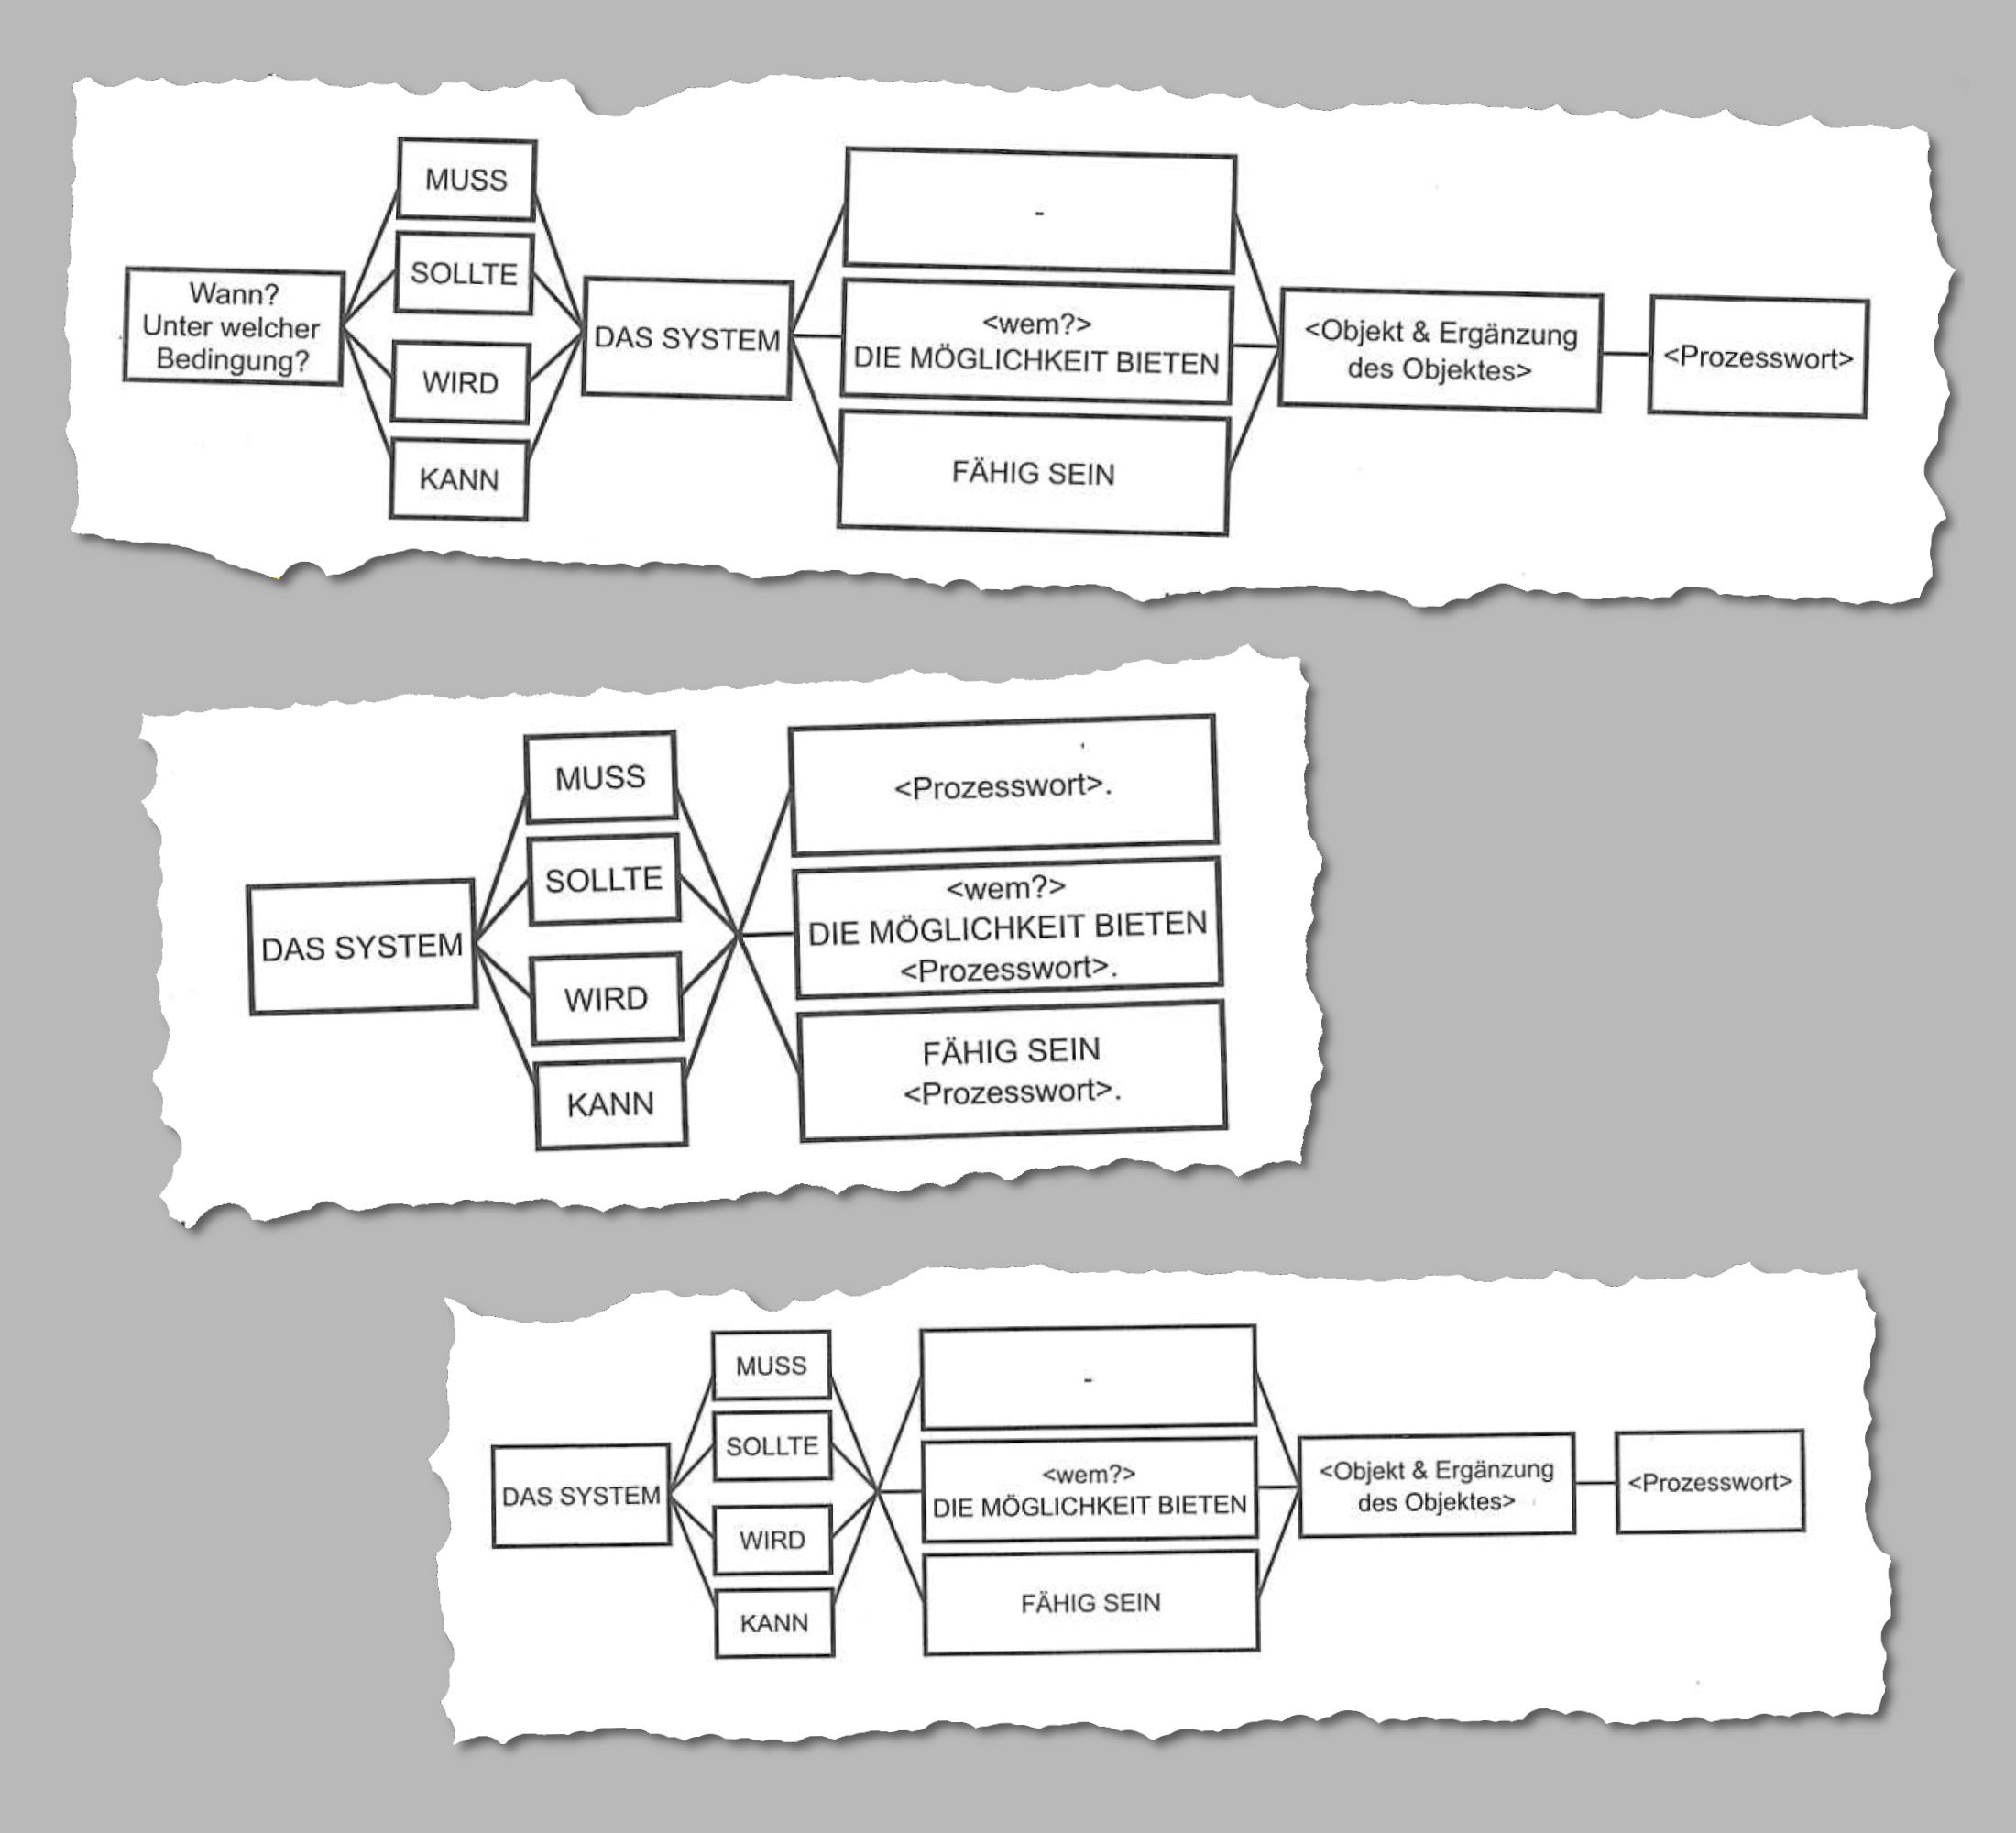
\includegraphics[width=\textwidth]{Bilder/Kapitel-6/Satzschablonen_Medley_V2.png}
	\caption[Satzschablonen]{Satzschablonen \cite[59 \psqq]{poh15}}
	\label{fig:satzschablone_fuer_systemanforderungen}
\end{figure}

\minisec{User Stories}

Insbesondere im agilen Umfeld wird für Nutzeranforderungen -- vor allem wenn sie extern sichtbares Verhalten des Systems betreffen -- eine leicht standardisierte Form gewählt, die beinhaltet, aus dem Blickwinkel welcher Personengruppe die Anforderung gestellt wird und auch explizit angibt, \textbf{warum} die Anforderung gestellt wird:

\sttpAnforderungText{"`Als [Rollenbezeichnung] möchte ich [Aktion], um [Zweck/Ziel/Bedürfnis]"'.}

Zum Beispiel: 

\sttpAnforderungText{"`Als oberster Tierpfleger im Zoo möchte ich die Urlaubs- und Abwesenheitszeiten der Tierpfleger einsehen können, um die wöchentlichen Dienstpläne der Tierpfleger zu erstellen"'.}

Eine solche Anforderungsformulierung nennt man eine \textit{User Story}. User Stories umfassen in der Regel einen oder zwei Sätze und werden in natürlicher Sprache formuliert, häufig in der dargestellten leicht strukturierten Form. Anders als bei den oben erwähnten Satzschablonen ist bei dieser agilen Form einer "`Schablone"' der Aufbau einer Anforderung nur sehr schwach vorstrukturiert. Insbesondere die Aktion, die die Rolle ausführen können möchte, kann in sehr unterschiedlichem Detaillierungsgrad in Form individueller Prosa beschrieben werden. Die Formulierung als User Story erfordert für die Anforderungssteller kaum Einarbeitungsaufwand. Zudem ist sie sehr auf die Arbeitsprozesse und Bedürfnisse des konkreten Anforderungsstellers fokussiert. Dieser explizite Bezug zur Rolle hat den Vorteil, dass unmittelbar deutlich ist, für welche Gruppe eine Funktionalität gewünscht wird. Ein gewisser Motivations\-aspekt für die Anforderungssteller ("`Ich beschreibe die Wünsche \textbf{meiner} Rolle"') ist zusätzlich gegeben.

\vspace{2.5mm} %%% für Druck

So bequem und motivationsfördernd eine solche, nur leicht vorstrukturierte, Erfassung von Anforderungen für die Anforderungssteller ist, desto komplizierter kann sie für den Requirements Engineer, den Product Owner, den Projektleiter oder die sonstige Rolle werden, die die Strukturierung und Priorisierung der Anforderungen im konkreten Softwareentwicklungsprojekt vornimmt: Durch die Fokussierung einer Anforderung auf die Bedürfnisse einer einzelnen Rolle wird der gesamte Prozess der Erfassung von Anforderungen auf einer kleinschrittigen Mikroebene organisiert. Gerade in Projekten mit vielen unterschiedlichen (Nutzer)Rollen kann eine anschließend gewünschte Zuordnung der erfassten Anforderungen zu größeren inhaltlichen Gruppen sehr aufwändig werden. Die unterschiedlichen Anforderungen müssen verglichen und gemeinsame Wünsche, aber auch Inkonsistenzen erkannt werden. Zum Beispiel wird im Zookontext die Rolle oberster Tierpfleger nicht die einzige sein, die Informationen zu den Abwesenheitszeiten der Tierpfleger für ihre Arbeit benötigt. Jede der anderen Rollen (\zb Tierarzt, Tierfütterungsorganisator, Personalverwaltung) wird eine ähnliche Anforderung zu diesem Kontext stellen, aber möglicherweise mit anderer Schwerpunktsetzung und sicher anders formuliert.

\vspace{2.5mm} %%% für Druck

In einem stark agil orientierten Projekt, bei dem die ständige iterative Anpassung sowohl der Anforderungen als auch ihrer Umsetzung in Programmcode zum Tages\-geschäft gehört, würde man zu Beginn des Projekts eine Zuordnung der Anforderungen zu größeren Gruppen gar nicht zwingend vornehmen wollen bzw. können, da die Sammlung weiterer Anforderungen parallel zur Umsetzung schon bestehender Anforderungen weiter läuft. Ein rollenzentriertes kleinschrittiges Vorgehen ist in solchen Projekten daher nicht von Nachteil -- und für solche Projekte sind User \mbox{Stories} auch eingeführt worden. Für Projekte, in denen der Großteil der Anforderungen schon zu Projektbeginn festgelegt werden soll, wird die rollenzentrierte kleinschrittige Erfassung der Anforderungen dagegen maximal der erste Schritt auf dem Weg zur Anforderungsspezifikation sein. %TODO:hier Verweis auf Storymap, wenn nicht in 5.3

\vspace{2.5mm} %%% für Druck

Unbestreitbar sinnvoll -- unabhängig vom gewählten Vorgehensmodell -- ist die in einer User Story vom Anforderungssteller verlangte Angabe des Zwecks seiner Anforderung. Auf diese Weise kann bei der Priorisierung von Anforderungen besser eingeschätzt werden, welche Folgen die Nichtberücksichtigung einer konkreten Anforderung hätte.

\minisec{Grafische Modelle}

Irgendwann im Laufe eines Softwareentwicklungsprozesses kommt der Zeitpunkt, zu dem man von der Ebene natürlichsprachlicher Beschreibungen auf die Ebene von \mbox{Modellen} wechselt. Das kann erst spät erfolgen, wie in vielen agilen Projekten, in denen die Bedürfnisse aus natürlichsprachlichen Anforderungen direkt in Programmcode für Funktionen umgesetzt werden, die diese Bedürfnisse erfüllen. In anderen Projekten werden natürlichsprachliche Anforderungen im Zuge von Entwurfstätigkeiten in (Entwurfs)Modelle übersetzt und dabei verfeinert und erst letztere Modelle dann in Programmcode umgesetzt. Grafische Modelle schon für die Anforderungsermittlung einzusetzen, kann man insofern auch als vorbereitende Arbeiten für Aufgaben ansehen, die man später sowieso erledigen müsste. Die während des Require\-ments Engineering entstandenen Modelle werden dann zu verfeinerten Modellen für Entwurfsbelange weiterentwickelt.

\vspace{1mm} %%% für Druck

Und so werden auch grafische Modelle im Requirements Engineering eingesetzt, um Anforderungen zu erfassen, zum Beispiel in folgenden Kontexten:

\begin{itemize}
	\item Domänenbasierte Anforderungen werden häufig in Form von Klassendiagrammen erfasst. 
	\item Das extern sichtbare Verhalten des Softwaresystems für seine unterschiedlichen Nutzergruppen kann über UML-Anwendungsfalldiagramme erfasst werden.
	\item Geschäftsprozesse, die das zukünftige Softwareprodukt durchführen oder unterstützen soll, werden ebenfalls oft grafisch dargestellt. Aus dem UML-
	\linebreak %%% für Druck
	Universum bieten sich hierfür Aktivitätsdiagramme an. Außerhalb der UML existieren zudem einige spezifische Notationen für die Darstellung von 
	\linebreak %%% für Druck
	Geschäfts\-prozessen.
	\item Anforderungen an die Schnittstellen zu anderen Systemen können über das in Abschnitt~\ref{sec:Kap-6.1.3.1} erwähnte Kontextdiagramm erfasst werden, indem dieses um die Informations- und Datenflüsse zwischen den Systemen ergänzt wird.
\end{itemize}

\vspace{1mm} %%% für Druck

Die gerade aufgezählten Arten von Anforderungen könnten grundsätzlich auch durch textuelle Formen (Prosa oder Satzschablonen) erfasst werden. Der Vorteil von grafischen Modellen gegenüber der natürlichen Sprache ist ihr höherer Grad an Eindeutigkeit, weil sie in der Regel viel weniger Interpretationsspielraum zulassen als natürliche Sprache. Zudem lassen sich Anforderungen, die man textuell sehr ausführlich beschreiben müsste (\zb komplexe Geschäftsprozesse) häufig mit grafischen Modellen einfacher und übersichtlicher darstellen. Ein Nachteil für die Adressaten ist der Einarbeitungsaufwand in die verwendete Modellierungssprache. Ein weiterer Nachteil ist der höhere Aufwand für die Pflege und Anpassung von Modellen: Eine natürlichsprachliche Anforderung kann mit wenig Aufwand umformuliert werden. Bei einer Anforderung, die Teil eines Modells ist, müssen bei jeder Änderung die Einhaltung der syntaktischen und semantischen Regeln der Modellierungssprache und die Auswirkungen auf andere Anforderungen im Modell berücksichtigt werden.

\vspace{1mm} %%% für Druck

Letzterer Aspekt adressiert schon einen grundlegenden Unterschied im Einsatzzweck zwischen der Verwendung textueller (vor allem natürlichsprachlicher) Formulierungen und der Verwendung von grafischen Modellen: Grafische Modelle werden häufig in Situationen eingesetzt, in denen weniger eine einzelne Anforderung im Fokus steht, als vielmehr Gruppen von Anforderungen und ihre Beziehungen zueinander betrachtet werden. Zusammenhänge zwischen einzelnen Anforderungen würden sich zwar auch in natürlichsprachlichen Formulierungen ausdrücken lassen, aber grafische Modelle bieten hier eine deutlich bessere Übersichtlichkeit. Auf diese Weise können widerstreitende Anforderungen einfacher erkannt werden oder zum Beispiel auch (Geschäfts)Bereiche identifiziert werden, aus denen bisher nur wenige Anforderungen vorliegen. In der Praxis werden grafische Modellform und textuelle Formulierungen häufig kombiniert, um die grafischen Modelle mit zusätzlichen Informationen anzureichern. Letztere werden dann aber meist in einer strukturierten textuellen Form und nicht in Prosa erfasst.

\vspace{2mm} %%% für Druck

\minisec{Das Anforderungsdiagramm von SysML}

\vspace{1mm} %%% für Druck

Wir haben oben kurz skizziert, welche UML-Diagramme man für die Erfassung verschiedener Arten von Anforderungen einsetzen kann. Ein spezifisches Anforderungsdiagramm besitzt die UML nicht. Ein solches findet sich allerdings in der Systems Modeling Language (SysML, \url{https://www.omgsysml.org/}), die im Jahr 2007 ebenfalls von der OMG veröffentlicht wurde. Während die UML schwerpunktmäßig auf die reine Softwareentwicklung ausgerichtet ist, nimmt die SysML mit der kompletten Systementwicklung (Software, Hardware, Elektronik und Mechanik) technischer Systeme ein deutlich größeres Anwendungsgebiet in den Blick. Die SysML wird heute häufig in Kombination mit Vorgehensweisen der modellgetriebenen System\-entwicklung eingesetzt, für die Systemzusammenhänge aufgrund automatisierter Verarbeitungsschritte auch formal spezifiziert werden müssen. 

\vspace{1mm} %%% für Druck

Für die SysML wurden bestehende UML-Diagramme angepasst und manche -- wie das Anforderungsdiagramm -- neu eingeführt. Die Anforderungen selber werden in einem, an das UML-Klassenelement angelehnten, Element aufgeschrieben und sind so in einer grafisch-textuellen Mischform dargestellt. Ein Vorteil des Anwendungsfalldiagramms ist, dass im selben Diagramm sowohl die Anforderungen und ihre Beziehungen untereinander, als auch Beziehungen zu Elementen anderer UML-Diagrammarten, wie zum Beispiel Anwendungsfälle, modelliert werden können. Das Anforderungsdiagramm kann somit auch Inhalte mehrerer Diagramme und ihre \mbox{Zusammenhänge} in einer Übersicht vereinen. Allerdings wird es dadurch auch deutlich komplexer, schwieriger zu erstellen und weniger intuitiv zu verstehen. In reinen Softwareentwicklungsprojekten wird das SysML-Anforderungsdiagramm daher auch eher selten eingesetzt -- insbesondere kaum für Diskussionen mit den Kunden. Hilfreich kann es für interne Diskussionen des Entwicklungsteams sein, um Abhängigkeiten zwischen verschiedenen nichtfunktionalen Anforderungen zu visualisieren oder Auswirkungen nichtfunktionaler Anforderungen auf funktionale Anforderungen darzustellen. 

\vspace{1mm} %%% für Druck

Eine kurze Übersicht zum SysML-Anforderungsdiagramm liefert \cite[51-53]{alt12}. Einen ausführlichen Blick auf das Diagramm und seine konkrete Verwendung im Rahmen eines vorgestellten Systementwicklungsmodells wirft \cite[234 \psqq]{wei14}.
\subsection{Die Anforderungsspezifikation}
\label{sec:Kap-6.2.4}

Eine Anforderungsspezifikation ist eine systematisch organisierte Sammlung von Anforderungen. Sie bildet die Gesamtheit der Anforderungen an das zu erstellende Softwareprodukt ab. Sie enthält somit sowohl die Nutzeranforderungen als auch die Systemanforderungen, allerdings nicht zwangsläufig in einem Dokument. Wenn der Auftrag zur Systementwicklung an einen externen Auftragnehmer vergeben wird, hat die Anforderungsspezifikation als Teil der Vertrags auch eine formelle Funktion. 

In nach klassischen Vorgehensmodellen organisierten Projekten besteht die Anforderungsspezifikation in der Regel aus dem sogenannten Lastenheft und dem sogenannten Pflichtenheft. \marginline{Lastenheft} Das Lastenheft ist ein strukturiert aufgebautes Dokument, das beschreibt, welche Anforderungen das Softwareprodukt erfüllen soll und welche zusätzlichen Randbedingungen bezüglich des Produkts oder auch des Entwicklungsprozesses gelten müssen. Das Lastenheft wird vom Auftraggeber erstellt (ggf. mit externer Unterstützung) und enthält mindestens Nutzeranforderungen. Sofern es auch schon Systemanforderungen umfasst, werden diese in der Regel durch das Pflichtenheft noch detaillierter spezifiziert. Oft ist das Lastenheft die Grundlage für eine Angebotseinholung bei potenziellen Auftragnehmern. Auftraggeber können sich für die Struktur eines Lastenhefts an vorhandenen Standards von Normierungs\-organisationen oder Vorgaben aus Vorgehensmodellen orientieren. In der Regel enthält ein Lastenheft mindestens folgende thematische Abschnitte:

\begin{itemize}
	\item Einführende Informationen und eine allgemeine Beschreibung des Produkts inklusive der Motivation. Hier würden die Informationen zu Zielen, Systemkontext und Produktumfang Platz finden.
	\item die funktionalen und nichtfunktionalen Anforderungen
	\item produktbezogene Rahmenbindungen, ggf. auch projektbezogene Rahmen-
	\linebreak %%% für Druck
	bedingungen
	\item Glossar der im Lastenheft verwendeten Begriffe der Domäne
	\item eine Übersicht über alle in der Spezifikation referenzierten Dokumente
\end{itemize}

Das Pflichtenheft 
\marginline{Pflichtenheft} 
ist mindestens eine Konkretisierung der Anforderungen aus dem Lastenheft. Darüber hinaus kann es aber sehr unterschiedlich gestaltet sein. So kann es außer den Systemanforderungen auch schon sehr konkrete Umsetzungsbeschreibungen für die Anforderungen aus dem Lastenheft enthalten oder einen groben Überblick über die geplante Systemarchitektur. 

In agilen Projekten wird häufig kein formelles Spezifikationsdokument erstellt. Stattdessen wäre die Anforderungsspezifikation im Prinzip die Sammlung aller User \mbox{Stories} oder die Gesamtheit der Items aller Sprint Backlogs. Oft wird aber die Notwendigkeit einer Gesamtspezifikation grundsätzlich in Frage gestellt und eher auf die zeitlich kürzere Dimension der Iterationen fokussiert. Die in einer Iteration umzusetzenden Anforderungen würden dann die Spezifikation dieser Iteration bilden. Für die Gesamtheit der nichtfunktionalen Anforderungen findet man aber auch in agilen Projekten häufiger strukturierte Spezifikationsdokumente.





% 6.3
\clearpage
\section{Anforderungen ermitteln und dokumentieren}
\label{sec:Kap-6.3}

Ein nicht zu unterschätzendes Problem in Softwareentwicklungsprojekten ist, wenn Auftraggeber und/oder Entwicklungsteam zu naiv davon ausgehen, dass der Auftrag\-geber genau weiß, was er möchte; dass alle Anforderungen, die er im Vorfeld schon aufgeschrieben hat vollständig und verständlich sind; und dass maximal noch die Bedeutung einiger vorkommender Fachbegriffe geklärt werden muss, bevor mit dem Entwurf für das Softwareprodukt begonnen werden kann. Nachdem seit den 2000er Jahren der Prozess des Requirements Engineering immer stärker in den Vordergrund gerückt ist, ist heute -- auch in sequentiell arbeitenden Software\-entwicklungs\-projekten -- eine ganz strikte Aufgabentrennung „der Kunde erstellt die Anforderungen, das Entwicklungsteam setzt sie um“ nicht mehr der Regelfall. Die Bedeutung des gemeinsam von Auftraggeber und Entwicklungsteam durchgeführten systema\-tischen Requirements Engineering für den Erfolg des Projekts wird aber trotzdem oft noch unterschätzt.

Wie in Lektion~1 % todo Lektion~\ref{sec:Lektion-1}
in Zusammenhang mit den Vorgehensmodellen schon angesprochen, ist die Vertragsgestaltung zwischen Auftraggeber und Entwicklungsprojekt durchführendem Auftragnehmer schwierig, wenn für den Vertragsabschluss keine formell spezifizierten Anforderungssammlungen vorliegen. Und dieser Aspekt steht im Wider\-spruch zu einem gemeinsam von Aufraggeber und Auftragnehmer durchgeführten Requirements Engineering. Unternehmen gehen mit dieser Problematik unterschiedlich um. Manche haben eigene Mitarbeiter oder sogar ganze Abteilungen, die sich auf Requirements Engineering spezialisiert haben und die Fachprojekte des Hauses bei der Erstellung von Anforderungsspezifikationen für Auftragsvergaben unterstützen. Andere Unternehmen führen für die Ermittlung von Anforderungen ein Vorprojekt vor dem eigentlichen Entwicklungsprojekt durch und lassen sich dabei von externen Requirements Engineering-Experten unterstützen. Im agilen Umfeld findet man zudem teilweise auch abweichende Vertragsmodelle, die versuchen, der Problematik von der anderen Richtung aus zu begegnen.

Zur Ermittlung von Anforderungen kann man ganz klassische Techniken aus dem Umfeld der Ist- und Soll-Analysen des Projektmanagements nutzen. Das können zum Beispiel der Einsatz von Fragebögen oder die Durchführung von Interviews sein, in denen die Stake\-holder über ihre Arbeitsabläufe, Organisationsstrukturen, vorhandene Probleme oder Wünsche an das neue Softwareprodukt befragt werden. Eine andere Möglichkeit ist, Beobachtungstechniken einzusetzen, wobei die konkreten Arbeitstätigkeiten der Stake\-holder vor Ort beobachtet, dokumentiert und anschließend gemeinsam analysiert werden, mit dem Ziel herauszufinden, an welchen Stellen das geplante Softwareprodukt unterstützen kann. Weiterhin ist der Einsatz von Brainstorming- und Kreativitätstechniken möglich. Bei letzteren sollte man die Stake\-holder allerdings nicht alleine lassen. Sinnvoll ist hier die gemein\-same Arbeit von Stake\-holdern und Requirements Engineering erfahrenen Personen (unternehmens\-intern oder externe Berater), um auch diesem kreativen Gedankenaustausch eine auf die Softwareproduktentwicklung zielführende Richtung zu geben. Eine Übersicht über konkrete Techniken aus diesen drei Bereichen finden Sie bei \cite[26-33]{poh15}.

\pagebreak %%% für Druck

Andere Techniken, die man zur Ermittlung und Dokumentation von Anforderungen einsetzen kann, entstammen spezifisch dem Softwareengineering-Bereich. Der folgende Abschnitt \ref{sec:Kap-6.3.1} stellt mit dem Anwendungsfalldiagramm eine überwiegend grafisch orientierte Möglichkeit aus dem UML-Umfeld vor.
\subsection{Anwendungsfälle modellieren}
\label{sec:Kap-6.3.1}

Bei der Modellierung von Anwendungsfällen (engl. use case) geht es darum, was Nutzer mit dem Softwareprodukt tun möchten bzw. tun. Anwendungsfälle werden daher verwendet, um ein Modell der Systemnutzung zu erstellen. \marginline{Modell der Systemnutzung} Dafür betrachten sie auf einer sehr hohen Abstraktionsebene die Interaktion verschiedener (potentieller) Nutzergruppen mit dem (zu erstellenden) Softwaresystem. Der Fokus liegt somit nur auf den extern sichtbaren Funktionalitäten des Systems und betrifft insofern eine Teilmenge der funktionalen Anforderungen. Über die Anwendungsfälle werden die Wünsche der Nutzer an die Software erfasst und dokumentiert. Das System selber wird als Blackbox behandelt, nur die Interaktion zwischen Nutzer und System wird betrachtet. Von den modellierten Anwendungsfällen ausgehend können dann im Entwurfsprozess der Software andere Arten von Diagrammen verwendet werden, um das dynamische Verhalten des Systems während der Interaktion mit dem Nutzer darzustellen. 

Das Anwendungsfalldiagramm der UML (engl.: use case diagram) basiert auf den Arbeiten von Ivar Jacobson in seiner Object-Oriented Software Engineering (OOSE)-Methode \cite{jac92}. Anwendungsfalldiagramme dienen in erster Linie der Kommunikation zwischen Nutzern und dem Softwareentwicklungsteam. Sie sind sehr einfach gehalten, damit sie auch von technisch nicht-versierten Nutzern verstanden und erstellt werden können. Abbildung~\ref{fig:fahrkartenautomat} zeigt ein erstes, noch sehr basales, UML-Anwendungsfalldiagramm.

%hier gehört abb Anwendungsfalldiagramm ("fig:fahrkartenautomat") eigentlich hin
\begin{figure}[h!]
	\vspace{\baselineskip} %%% für Druck
	\vspace{\baselineskip} %%% für Druck

	\centering
	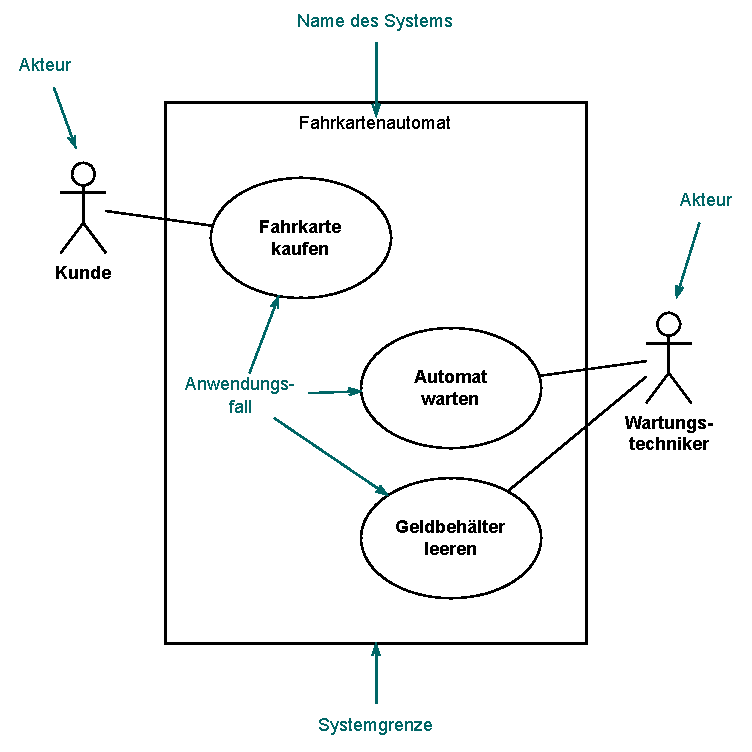
\includegraphics[scale=1.0]{Bilder/Kapitel-6/Fahrkartenautomat.pdf}	
	\caption[Ein UML-Anwendungsfalldiagramm]{Ein einfaches UML-Anwendungsfalldiagramm mit zwei Akteuren und drei Anwendungsfällen}
	\label{fig:fahrkartenautomat}
\end{figure}

Ein Anwendungsfalldiagramm besteht aus mindestens einem Anwendungsfall, der mit mindestens einem Akteur verbunden ist. Abbildung~\ref{fig:fahrkartenautomat} zeigt ein Anwendungsfalldiagramm mit zwei Akteuren (Kunde, Wartungstechniker), in UML-Notation dargestellt als Strichmännchen als Zeichen für menschliche Akteure. Außerdem sind drei Anwendungsfälle abgebildet, dargestellt als Ellipsen (keine Kreise!). Die Bezeichnung eines Anwendungsfalls wird üblicherweise als Tätigkeit formuliert.

Über die Verbindungen zwischen Akteuren und Anwendungsfällen wird modelliert, welche Akteure welche Anwendungsfälle ausführen. In der Abbildung ist der Akteur \sttpUMLText{Kunde} nur mit dem Anwendungsfall \sttpUMLText{Fahrkarte kaufen} verbunden, er kann also die beiden anderen Anwendungsfälle \sttpUMLText{Automat warten} und \sttpUMLText{Geldbehälter leeren} nicht ausführen. Dies soll nur der Akteur \sttpUMLText{Wartungstechniker} können, daher bestehen Verbindungen vom Akteur Wartungstechniker zu diesen zwei Anwendungsfällen.

Ein \marginline{Akteur} Akteur in einem Anwendungsfalldiagramm modelliert eine Rolle, die konkrete Nutzer bei der Benutzung des Systems annehmen können. Akteure bilden also keine Nutzer ab, sondern nur eingenommene Rollen bei der Systemnutzung. So könnte zum Beispiel ein realer Nutzer des Systems in der Rolle \sttpUMLText{Kunde} eine Fahrkarte kaufen, \textbf{dieselbe} Person in der Rolle \sttpUMLText{Wartungstechniker} aber auch den Automaten warten oder den Geldbehälter leeren.

Jeder Anwendungsfall in einem Anwendungsfalldiagramm, der mit Akteur(en) verbunden ist, definiert eine Interaktionsschnittstelle zwischen dem System und einem oder mehreren Akteuren. Ein Anwendungsfall beschreibt eine abgeschlossene Funktionalität, die das System erbringen muss. Dabei wird aber nicht festgelegt, \textbf{wie} diese Funktionalität erbracht werden soll und auch nicht zwangsläufig (\su) aus wie vielen und welchen einzelnen Aktionen die Interaktion zwischen Akteur(en) und System besteht. Üblicherweise bildet man die Anwendungsfälle aus Sicht der Akteure so, dass jeder Anwendungsfall einen erkennbaren Nutzen für die beteiligten Akteure erbringt. Von Einzelheiten auf dem Weg zu diesem Nutzen kann auch abstrahiert werden. So wird zum Beispiel der Anwendungsfall \sttpUMLText{Fahrkarte kaufen} vermutlich aus mehreren Interaktionen zwischen Akteur \sttpUMLText{Kunde} und dem System bestehen (\mbox{Züge} aussuchen, Tarif auswählen, Geld einzahlen etc.). Diese Menge an Aktionen wird hier in Abbildung~\ref{fig:fahrkartenautomat} in dem Anwendungsfall \sttpUMLText{Fahrkarte kaufen} gebündelt, der dem Akteur \sttpUMLText{Kunde} einen erkennbaren Nutzen, nämlich die gekaufte Fahrkarte, erbringt.

\pagebreak %%% für Druck

Da Anwendungsfälle Interaktionsschnittstellen der (späteren) Nutzer mit dem System sind, werden im Rahmen der Anforderungsermittlung in einem Anwendungsfalldiagramm nur solche Tätigkeiten der Nutzer berücksichtigt, die relevant für das System sind. Beispiel aus dem Zookontext: In der Realwelt füttert ein Tierpfleger Tiere. Ein Anwendungsfall \sttpUMLText{Tiere füttern} würde sich aber nur dann in einem Anwendungsfalldiagramm der Anforderungsermittlung für die Zooverwaltungssoftware finden, wenn die zukünftige Software diese Tätigkeit in irgendeiner Weise unterstützen (\zb automatisierte Futterbeschaffung), planen (\zb Planung der Fütterungszeiten), dokumentieren (\zb Übersicht über ausgegebene Futtermenge) etc. soll. (Bei der Nutzung von Anwendungsfalldiagrammen im Rahmen der Domänenmodellierung kann das auch anders sein, \su)

Neben den Akteuren und den Anwendungsfällen ist in Abbildung~\ref{fig:fahrkartenautomat} auch eine System\-grenze
\marginline{Systemgrenze} 
(viereckige Umrandung mit Angabe des Systemnamens) eingezeichnet. Alle Elemente, die sich innerhalb der Systemgrenze befinden, gehören zum System. Dies sind die Anwendungsfälle, für die das System entsprechende Funktionalität bereitstellen muss. Die Akteure als diejenigen, die mit dem System interagieren, werden außerhalb der Systemgrenze eingezeichnet. Wo genau sie außerhalb der System\-grenze platziert werden, ist nicht vorgegeben. Wir haben den Akteur \sttpUMLText{Kunde} in der Abbildung links des Systems und den Akteur \sttpUMLText{Wartungstechniker} rechts angeordnet. Üblicherweise orientiert man sich daran, bei welcher Platzierung sich die übersichtlichsten Verbindungen zu den Anwendungsfällen ziehen lassen.

Das Einzeichnen der Systemgrenze ins Anwendungsfalldiagramm ist nach UML-Regeln optional. Sinnvoll ist die Angabe der Systemgrenze in einem Anwendungsfalldiagramm insbesondere in den Fällen, in denen das betrachtete System nicht nur mit verschiedenen menschlichen Akteuren, sondern auch mit anderen technischen Systemen interagiert bzw. interagieren soll.

Bei den in UML-Anwendungsfalldiagrammen betrachteten Systemen kann es sich um reine Hardwaresysteme, reine Softwaresysteme oder eine Kombination von beidem handeln. Im Rahmen des Softwareengineering wird man eher selten reine Hardwaresysteme betrachten. Das in Abbildung~\ref{fig:fahrkartenautomat} dargestellte System mit Namen \sttpUMLText{Fahrkartenautomat} beinhaltet sowohl Hardware- als auch Softwarekomponenten. Anwendungsfalldiagramme abstrahieren jedoch davon, welche Komponente des (zukünftigen) Systems welchen der dargestellten Anwendungsfälle  übernehmen bzw. unterstützen soll. Insofern unterscheidet sich die Struktur eines Anwendungsfall\-diagramms für ein kombiniertes Hard-/Softwaresystem wie den Fahrkartenautomaten nicht von einem reinen Softwaresystem wie dem Online-Fahrkartenkauf in der nächsten Abbildung.

\minisec{Beziehungen zwischen Anwendungsfällen}

Abbildung~\ref{fig:fahrkartenautomat_online} zeigt für einen Anwendungsfall \sttpUMLText{Fahrkarte kaufen} ein verfeinertes Anwendungsfalldiagramm, in dem weitere typische Elemente vorkommen.

%%% Hier gehört Abbildung "fig:fahrkartenautomat_online" eigentlich hin.

Neben dem Anwendungsfall \sttpUMLText{Fahrkarte kaufen} befinden sich in dem Diagramm einige weitere als Ellipsen dargestellte Anwendungsfälle, die alle direkt oder indirekt mit \sttpUMLText{Fahrkarte kaufen} verbunden sind. Über die Beziehungstypen \sttpUMLText{<<include>>} und \sttpUMLText{<<extend>>} lassen sich inhaltliche Abhängigkeiten zwischen verschiedenen Anwendungsfällen modellieren.

\pagebreak %%% für Druck

\begin{figure}[h!]
	\begin{addmargin*}[0cm]{-\marginparwidth}
		\begin{addmargin*}[0cm]{-\marginparsep}
			\vspace{5mm} %%% für Druck
			\centering
			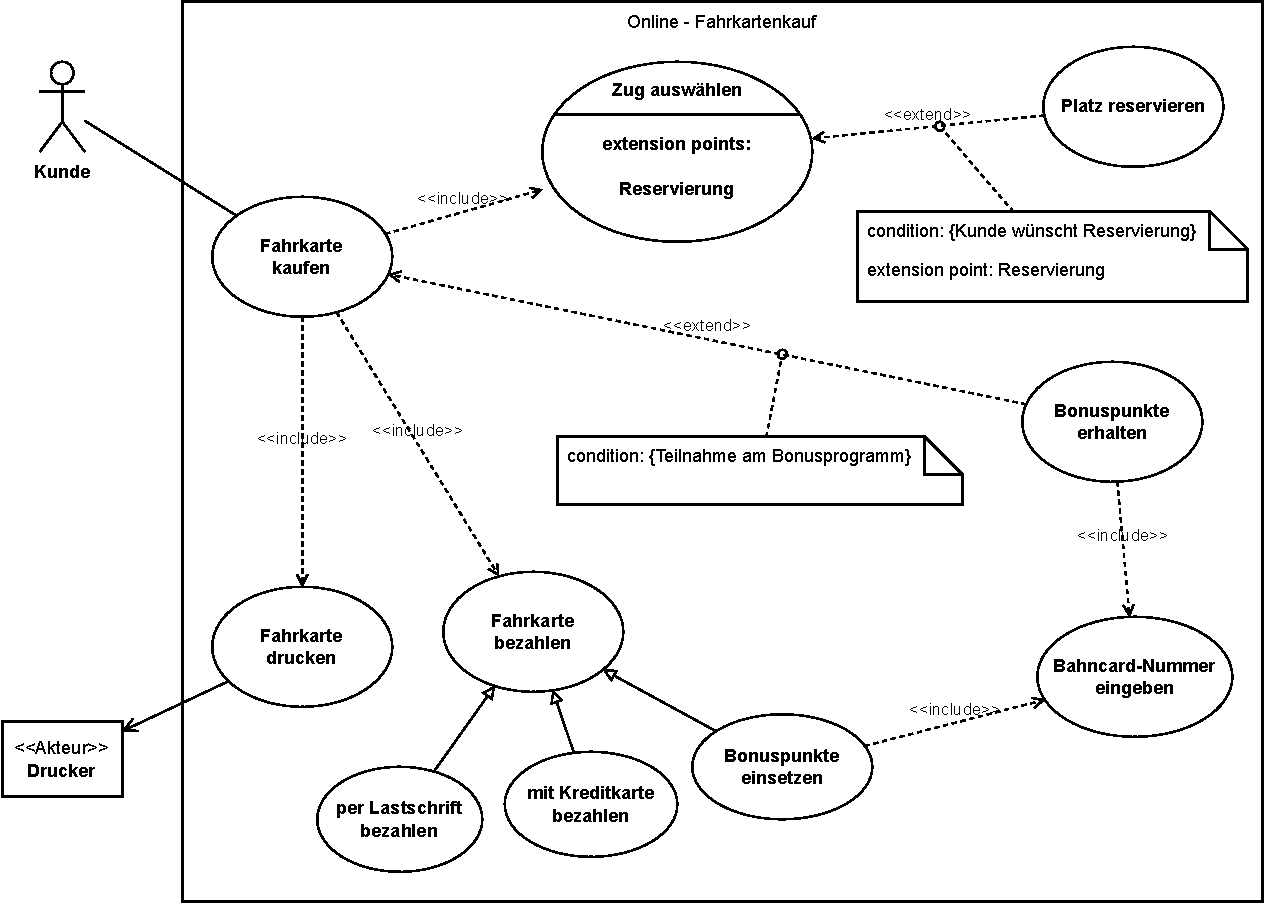
\includegraphics[scale=0.8]{Bilder/Kapitel-6/Fahrkartenautomat-online.pdf}
			\vspace{3mm} %%% für Druck
			\caption{Anwendungsfalldiagramm Online-Fahrkartenkauf}
			\label{fig:fahrkartenautomat_online}
		\end{addmargin*}
	\end{addmargin*}
\end{figure}

Alle \marginline{<<include>>} Anwendungsfälle, die über eine \sttpUMLText{<<include>>}-Beziehung mit dem Anwendungsfall \sttpUMLText{Fahrkarte kaufen} verbunden sind, gehören mit zur Funktionalität \sttpUMLText{Fahrkarte} \sttpUMLText{kaufen}. Man sagt: sie sind in die Funktionalität des Anwendungsfalls \sttpUMLText{Fahrkarte} \sttpUMLText{kaufen} \textbf{eingebunden}. In Abbildung~\ref{fig:fahrkartenautomat_online} sind also die Anwendungsfälle \sttpUMLText{Fahrkarte} \sttpUMLText{drucken}, \sttpUMLText{Fahrkarte} \sttpUMLText{bezahlen} und \sttpUMLText{Zug} \sttpUMLText{auswählen} in den Anwendungsfall
\linebreak %%% für Druck
\sttpUMLText{Fahrkarte} \sttpUMLText{kaufen} eingebunden. Die Anforderung an das zu erstellende Software\-produkt ist somit, dass jedes Mal, wenn eine Fahrkarte gekauft wird, auch alle Aktionen, die in den drei eingebundenen Anwendungsfällen spezifiziert sind, stattfinden müssen. Beachten Sie die (unter Umständen) etwas irritierende Mehrfach-Verwendung des Begriffs "`Anwendungsfall"' in Anwendungsfalldiagrammen: Jede \mbox{Ellipse} in einem Anwendungsfalldiagramm ist ein Anwendungsfall. Es wird begrifflich nicht unterschieden, ob es sich um einen eingebundenen Anwendungsfall oder um einen direkt mit dem Akteur verbundenen "`Haupt"'-Anwendungsfall handelt.

Über die Verwendung von \sttpUMLText{<<include>>} kann ein stark abstrahierter Anwendungsfall wie \sttpUMLText{Fahrkarte kaufen} in seine Teilinteraktionen zwischen Akteur und System verfeinert werden. Gleichzeitig können auf diese Weise Anwendungsfälle beschrieben werden, die identische Teilfunktionalitäten erfordern. Letztere werden dafür als eigenständiger Anwendungsfall modelliert, der in andere Anwendungsfälle eingebunden werden kann. Zum Beispiel binden die beiden Anwendungsfälle \sttpUMLText{Bonuspunkte} \sttpUMLText{erhalten} und \sttpUMLText{Bonuspunkte} \sttpUMLText{einsetzen} in Abbildung~\ref{fig:fahrkartenautomat_online} beide den Anwendungsfall \sttpUMLText{Bahncard-Nummer eingeben} ein. Genauso könnte auch ein von \sttpUMLText{Fahrkarte kaufen} völlig unabhängiger Anwendungsfall, wie zum Beispiel das Verlängern einer Bahncard, den schon im Rahmen von \sttpUMLText{Fahrkarte} \sttpUMLText{kaufen} spezifizierten Anwendungsfall \sttpUMLText{Bahncard-Nummer eingeben} einbinden. Auf diese Weise können Anwendungsfälle mit Teilfunktionalitäten für denselben oder andere Akteure wiederverwendet werden.

\vspace{1mm} %%% für Druck
 
Beachten Sie: Über die Verbindungen zwischen \sttpUMLText{Fahrkarte kaufen} und allen anderen Anwendungsfällen ist auch der Akteur \sttpUMLText{Kunde} indirekt mit allen Anwendungs\-fällen verbunden. Er kann letztere allerdings nicht unabhängig von \sttpUMLText{Fahrkarte} 
\linebreak %%% für Druck
\sttpUMLText{kaufen} initiieren. So ist zum Beispiel durch die Modellierung in Abbildung~\ref{fig:fahrkartenautomat_online} nicht vorgesehen, dass der Akteur \sttpUMLText{Kunde} einen Platz im Zug reservieren kann, ohne eine Fahrkarte zu kaufen. Sollte das eine Anforderung an das zu erstellende Software\-produkt sein, so muss der Akteur \sttpUMLText{Kunde} mit dem Anwendungsfall \sttpUMLText{Platz} \sttpUMLText{reservieren} zusätzlich direkt verbunden werden.

\vspace{1mm} %%% für Druck

Eine zweite, häufig eingesetzte Beziehungsart zwischen Anwendungsfällen ist die \sttpUMLText{<<extend>>}-Beziehung.
\marginline{<<extend>>} 
Wie die \sttpUMLText{<<include>>}-Beziehung wird sie durch einen gestrichelten Pfeil dargestellt (Vorsicht: umgekehrte Pfeilrichtung!). Die \sttpUMLText{<<extend>>}-Beziehung modelliert eine bedingte Einbindung von Anwendungsfällen, man sagt auch: sie \textbf{erweitert} den einbindenden Anwendungsfall. In Abbildung~\ref{fig:fahrkartenautomat_online} wird der Anwendungs\-fall \sttpUMLText{Fahrkarte kaufen} durch den Anwendungsfall \sttpUMLText{Bonuspunkte erhalten} erweitert. Der Anwendungsfall \sttpUMLText{Zug} \sttpUMLText{auswählen} wird durch den Anwendungsfall \sttpUMLText{Platz} \sttpUMLText{reservieren} erweitert. Die \sttpUMLText{<<extend>>}-Beziehung zwischen Anwendungsfällen wird mit einer Bedingung (engl. condition) versehen. Diese Bedingung gibt an, unter welchen Voraussetzungen der Anwendungsfall eingebunden wird. Im Gegensatz zu \sttpUMLText{<<include>>} werden also über \sttpUMLText{<<extend>>} verbundene Anwendungsfälle nicht jedes Mal eingebunden. In der Abbildung wird der Anwendungsfall \sttpUMLText{Fahrkarte kaufen} genau dann durch den Anwendungsfall \sttpUMLText{Bonuspunkte erhalten} erweitert, wenn eine Teilnahme des Akteurs am Bonusprogramm vorliegt. Sofern diese Bedingung nicht zutrifft, soll die Funktionalität hinter \sttpUMLText{Bonuspunkte erhalten} nicht Teil der Funktionalität \sttpUMLText{Fahrkarte kaufen} sein. Die UML verbietet es nicht, \sttpUMLText{<<extend>>}-Verbindungen ohne Bedingung zu modellieren. In einem solchen Fall würde der erweiternde Anwendungs\-fall immer eingebunden, sich die \sttpUMLText{<<extend>>}-Beziehung also wie eine \sttpUMLText{<<include>>}-Beziehung verhalten. Eine solche Modellierung macht das Lesen eines Anwendungsfalldiagramms aber unnötig komplizierter. Daher: wenn \sttpUMLText{<<extend>>}, dann nur zusammen mit einer Bedingung!

\vspace{1mm} %%% für Druck

Man \marginline{Erweiterungs\-punkte} kann für eine \sttpUMLText{<<extend>>}-Beziehung neben der Bedingung noch sogenannte Erweiterungspunkte (engl. extension points) angeben. In Abbildung~\ref{fig:fahrkartenautomat_online} sehen Sie diese Konstruktion in der Beziehung zwischen \sttpUMLText{Zug} \sttpUMLText{auswählen} und \sttpUMLText{Platz} \sttpUMLText{reservieren}. Dafür werden im Anwendungsfall, der erweitert wird (\sttpUMLText{Zug} \sttpUMLText{auswählen}) unter einer horizontalen Linie die möglichen Erweiterungspunkte aufgeführt und gleichzeitig am Beziehungspfeil zusätzlich zur relevanten Bedingung angegeben. Diese 
\linebreak %%% für Druck
ausführlichere Modellierung der \sttpUMLText{<<extend>>}-Beziehung ist insbesondere dann sinnvoll, wenn ein Anwendungs\-fall an mehreren \sttpUMLText{<<extend>>}-Beziehungen beteiligt ist oder es zusätzlich zur grafischen Darstellung im Diagramm eine textuelle Beschreibung (s.u.) des Anwendungs\-falls und der \sttpUMLText{<<extend>>}-Beziehung geben soll.

In UML-Anwendungsfalldiagrammen kann auch die aus den Klassendiagrammen bekannte Generalisierung verwendet werden. Damit können Hierarchien zwischen 
\linebreak %%%für Druck
Anwendungsfällen modelliert werden. In Abbildung~\ref{fig:fahrkartenautomat_online} finden sich zum Anwendungsfall \sttpUMLText{Fahrkarte bezahlen} drei „Unter“-Anwendungsfälle. Man verwendet
\linebreak %%%für Druck
Generalisierungsbeziehungen in Anwendungsfalldiagrammen immer dann, wenn eine (Teil)Funktionalität des „Ober“-Anwendungsfalls bei seinen spezialisierten Anwendungsfällen verändert ist bzw. letztere zusätzliche Funktionalität beinhalten -- also analog zur Verwendung der Generalisierung in Strukturdiagrammen wie dem Klassen\-diagramm. Generalisierungsbeziehungen kann es zudem auch zwischen Akteuren in einem Anwendungsfalldiagramm geben. Zum Beispiel könnten die Akteure \sttpUMLText{Kunde} und \sttpUMLText{Wartungstechniker} aus Abbildung~\ref{fig:fahrkartenautomat} beide Spezialisierungen eines Akteurs \sttpUMLText{Person} sein. Gene\-rali\-sierungs-Kon\-struk\-tionen auf der Ebene von Akteuren machen dann Sinn, wenn es Anwendungsfälle gibt, die mehrere bzw. alle Akteure initi\-ieren können sollen, aber gleichzeitig auch Anwendungsfälle, die nur für spezifische Akteure relevant sind. Vorsicht: auch hier sollte man wie in allen Diagrammarten die Generalisierung nicht auf die Spitze treiben. (Berühmtes Beispiel zu Generalisierungssünden: Man sollte nicht Tische von Hunden ableiten, nur weil beide vier Beine haben.)

Das letzte noch nicht besprochene Element in Abbildung~\ref{fig:fahrkartenautomat_online} ist der Akteur \sttpUMLText{Drucker} unten links. Hier sehen Sie die Modellierung für einen nicht-menschlichen Akteur. Der Akteur Drucker ist mit dem Anwendungsfall \sttpUMLText{Fahrkarte drucken} verbunden. Eine solche Verbindung mit Pfeilspitze (gerichtete Verbindung) zum Akteur wird verwendet, wenn der Akteur am Anwendungsfall beteiligt ist, diesen aber nicht selber initiieren kann. Gerichtete Verbindungen sind nicht auf nicht-menschliche Akteure beschränkt.

\vspace{2mm} %%% für Druck

\minisec{Einsatzzweck und Grenzen}

Die Abbildung~\ref{fig:fahrkartenautomat} und die Abbildung~\ref{fig:fahrkartenautomat_online} zeigen unterschiedlich stark abstrahierte Modellierungen. Beide Formen können im Rahmen der Anforderungsermittlung hilfreich sein. Über ein Anwendungsfalldiagramm wie in Abbildung~\ref{fig:fahrkartenautomat} könnte man zunächst alle direkten Interaktionen zwischen Akteuren und dem zukünftigen System spezifizieren. Jeder im Diagramm aufgeführte Anwendungsfall wäre dann mit mindestens einem Akteur direkt verbunden. Es ist im Übrigen durchaus auch üblich, pro Akteur ein eigenes Diagramm anzufertigen, in dem nur die Anwendungsfälle aufgeführt sind, die von diesem Akteur ausgeführt werden sollen. Solche Anwendungsfall\-diagramme auf einem sehr hohen Abstraktionsniveau können (zukünftige) Nutzer auch gut noch ohne Hilfe des Entwicklungsteams erstellen, insbesondere dann, wenn jeder Nutzer nur die Anwendungsfälle für seine Rolle spezifizieren muss.

Für ein schon recht verfeinertes Diagramm wie in Abbildung~\ref{fig:fahrkartenautomat_online} ist es sinnvoll, wenn Stakeholder und Entwicklungsteam (bzw. einzelne Mitglieder des Entwicklungsteams) dieses gemeinsam erstellen, um Missverständnissen von Beginn an vorzubeugen. Denn hier wird schon detaillierter festgelegt, aus welchen Teil\-inter\-aktionen eine Interaktion zwischen Akteur und System bestehen soll. Aspekte, die hier vergessen oder falsch dargestellt werden, erfordern nachher vermutlich komplexere Änderungen an diesem und unter Umständen auch weiteren Diagrammen. Gleichzeitig werden solche detaillierteren Anwendungsfalldiagramme auch eingesetzt, um gemeinsame Teil\-inter\-aktionen verschiedener Anwendungsfälle zu finden. Insbesondere wenn es sich dabei um Anwendungsfälle unterschiedlicher Akteure handelt, sollte möglichst frühzeitig sichergestellt sein, dass alle Beteiligten unter der spezifizierten Teilinteraktion wirklich das identische Verhalten vom System erwarten. 

Die Verfeinerung eines Anwendungsfalls in Teilinteraktionen ist nicht auf Anwendungsfälle beschränkt, die direkt mit Akteuren verbunden sind. Jeder Anwendungsfall in Abbildung~\ref{fig:fahrkartenautomat_online} könnte noch weiter differenziert werden. So lassen sich über Anwendungsfalldiagramme schon sehr detailliert inhaltliche Abhängigkeiten zwischen (Teil)Interaktionen erfassen. Beim praktischen Einsatz sollte man allerdings zwei Punkte beachten. Zum einen sind Anwendungsfalldiagramme nicht dazu gedacht, Reihenfolgen der Interaktionen oder zeitliche Abfolgen festzulegen. Die sicher\-lich gewünschte Reihenfolge „erst Zug auswählen, dann Fahrkarte bezahlen, dann Fahrkarte drucken“ würde man nicht über ein Anwendungsfalldiagramm ausdrücken, sondern über andere Arten von Verhaltensdiagrammen. Zum anderen sollte man den Fokus auf die Akteure nicht verlieren. Das bedeutet, jede Ellipse im Anwendungsfall\-diagramm sollte eine echte (Teil)Interaktion zwischen System und Akteur sein. Tätig\-keiten, die das System „im Hintergrund“ ausführen muss, wie zum Beispiel die Gültigkeit der Bahncard zu prüfen oder die Platzreservierung zu speichern, gehören nicht in ein Anwendungsfalldiagramm.

\vspace{1mm} %%% für Druck

\minisec{Anwendungsfalldiagramme im Rahmen der Domänenmodellierung}

Auch für die Domänenmodellierung kann man Anwendungsfalldiagramme einsetzen, zum Beispiel wie in Abbildung~\ref{fig:anwendungsfall_tiere_fuettern}, um ein besseres Verständnis von Tätigkeiten von Akteuren in der Domäne zu bekommen. Dargestellt sind hier für die Tierpfleger der Nagetiere (links) und die Tierpfleger der Löwen (rechts) die Tätigkeiten, die diese rund um die Fütterung ihrer Tiere ausführen. Das „System“, mit dem die Akteure interagieren, ist die Domäne. Die Einzeichnung von Systemgrenzen würde hier eher verwirren, da die Akteure genau wie die Anwendungsfälle Teil der Domäne sind.

%%% Hier gehört die Abbildung "fig:anwendungsfall_tiere_fuettern" eigentlich hin.

Der Einsatz von Anwendungsfalldiagrammen zur Modellierung der Domäne ist nur dann sinnvoll, wenn es einen Bezug zum zu erstellenden Softwareprodukt gibt. Hier könnte der Modellierungszweck gewesen sein, die Stellen im aktuell manuell ablaufenden Fütterungsprozess zu identifizieren, die sich für eine softwareunterstützte Automatisierung eignen würden. Die Anwendungsfälle \sttpUMLText{Futter bestellen} und \sttpUMLText{Fütterung dokumentieren} wären denkbare Kandidaten. Die Modellierung über Anwendungsfälle reicht für diese Erkenntnis auch aus und kann von den Tier\-pflegern selbst erstellt werden. Eine detaillierte und schwieriger zu erstellende Darstellung der genauen Geschäftsprozesse der Domäne (z.B. über Aktivitätsdiagramme) könnte sich für diese Anwendungsfälle dann anschließen.

\vspace{1mm} %%% für Druck

\minisec{Anwendungsfälle textuell beschreiben}

Man kann Anwendungsfälle auch textuell beschreiben. Üblicherweise findet das nicht alternativ, sondern ergänzend zu Anwendungsfalldiagrammen statt. Ziel der textuellen Ergänzung ist immer, zusätzliche Informationen festzuhalten (zu Spezifikations- oder Dokumentationszwecken), die sich nicht aus dem Diagramm allein ergeben. 

\begin{figure}[h!]
	\begin{addmargin*}[0cm]{-\marginparwidth}
		\begin{addmargin*}[0cm]{-\marginparsep}
			\vspace{5mm} %%% für Druck
			\centering
			\begin{minipage}[c]{7.5cm} 
				\centering
				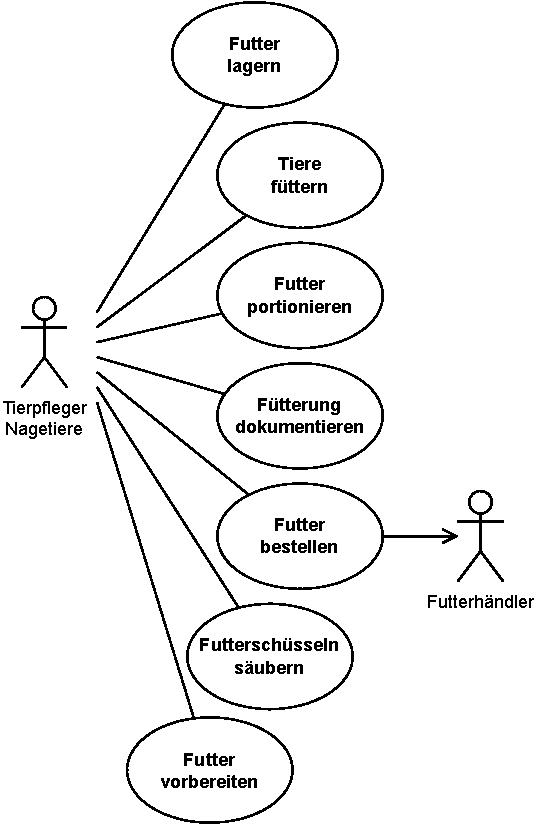
\includegraphics[scale=0.8]{Bilder/Kapitel-6/anwendungsfall_tiere_fuettern_nagetiere.pdf}
			\end{minipage}
			\begin{minipage}[c]{0.1cm} 
				\centering
				{\color{FernUni-MI-green}\rule{1pt}{90mm}} % senkrechte farbige Linie
			\end{minipage}
			\begin{minipage}[c]{9cm}
				\centering
				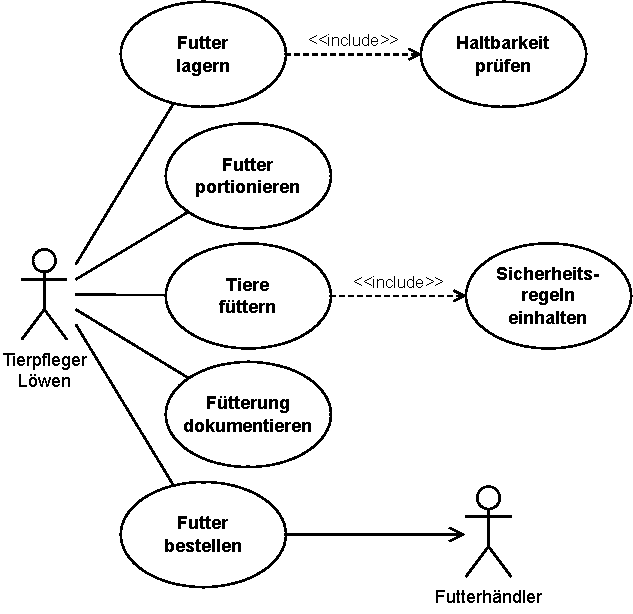
\includegraphics[scale=0.8]{Bilder/Kapitel-6/anwendungsfall_tiere_fuettern_loewen.pdf}
			\end{minipage}
			\vspace{\baselineskip} %%% für Druck
			\caption{Domänenmodellierung über Anwendungsfälle}
			\label{fig:anwendungsfall_tiere_fuettern}
		\end{addmargin*}
	\end{addmargin*}
\end{figure}

\vspace{1cm} %%% für Druck

Typische textuelle Ergänzungen sind die Angabe von Vor- und Nachbedingungen zu Anwendungsfällen oder einen Anwendungsfall auslösende Ereignisse. Zum Beispiel: Wann bzw. unter welchen Voraussetzungen wird der Anwendungsfall ausgeführt? Möglicherweise soll in Abbildung~\ref{fig:fahrkartenautomat_online} der Anwendungsfall \sttpUMLText{Fahrkarte kaufen} nur initiiert werden können, wenn der Akteur sich vorher im Buchungssystem registriert hat. 

Ein weiterer Einsatzzweck von textuellen Ergänzungen sind Erläuterungen zu im Diagramm vorkommenden Begriffen oder Konzepten. Beispiel Abbildung~\ref{fig:fahrkartenautomat_online}: Was sind Bonuspunkte? Und kann man die Bonuspunkte, die man beim Fahrkartenkauf erhalten würde direkt zum Kauf dieser Fahrkarte schon einsetzen? Ob man solche \mbox{Informationen} besser als textuelle Ergänzung zu einem Anwendungsfall-
\linebreak %%% für Druck
diagramm oder an anderer Stelle (z.B. textuell in einem Glossar oder in stärker ablauf\-orientierten anderen grafischen Diagrammen) festhält, ist sehr projektspezifisch -- in manchen agilen Vorgehensmodellen würde man sie gar nicht schriftlich festhalten, sondern nur mündlich kommunizieren.

Textuelle Ergänzungen werden häufig auch dafür verwendet, die Erweiterungen zum Standardablauf eines „Haupt“-Anwendungsfalls (alle Anwendungsfälle, die mit \mbox{<<extend>>} angebunden sind) detaillierter zu beschreiben. Auch hier gilt, dass als \mbox{Alternative} zur textuellen Ergänzung eines Anwendungsfalldiagramms auch der zusätzliche Einsatz anderer Verhaltensdiagramme (wie z.B. Aktivitätsdiagramme) 
\linebreak %%% für Druck
möglich ist.

Wenn man textuelle Ergänzungen zu Anwendungsfalldiagrammen sehr strukturiert und ausführlich aufschreiben möchte, findet man in der Literatur dafür zahlreiche Schablonen. Abbildung~\ref{fig:use_case_schablone} zeigt eine solche Schablone. Etwas anders strukturierte Schablonen finden Sie bei \cite[S. 172 und S. 193]{rup14} und \cite[98 \psq]{ber18}, bei letzterem auch Verweise auf weitere Literatur.

\vspace{\baselineskip} %%% für Druck

\begin{figure}[h!]
	\begin{addmargin*}[0cm]{-\marginparwidth}
	\begin{addmargin*}[0cm]{-\marginparsep}
		\centering
		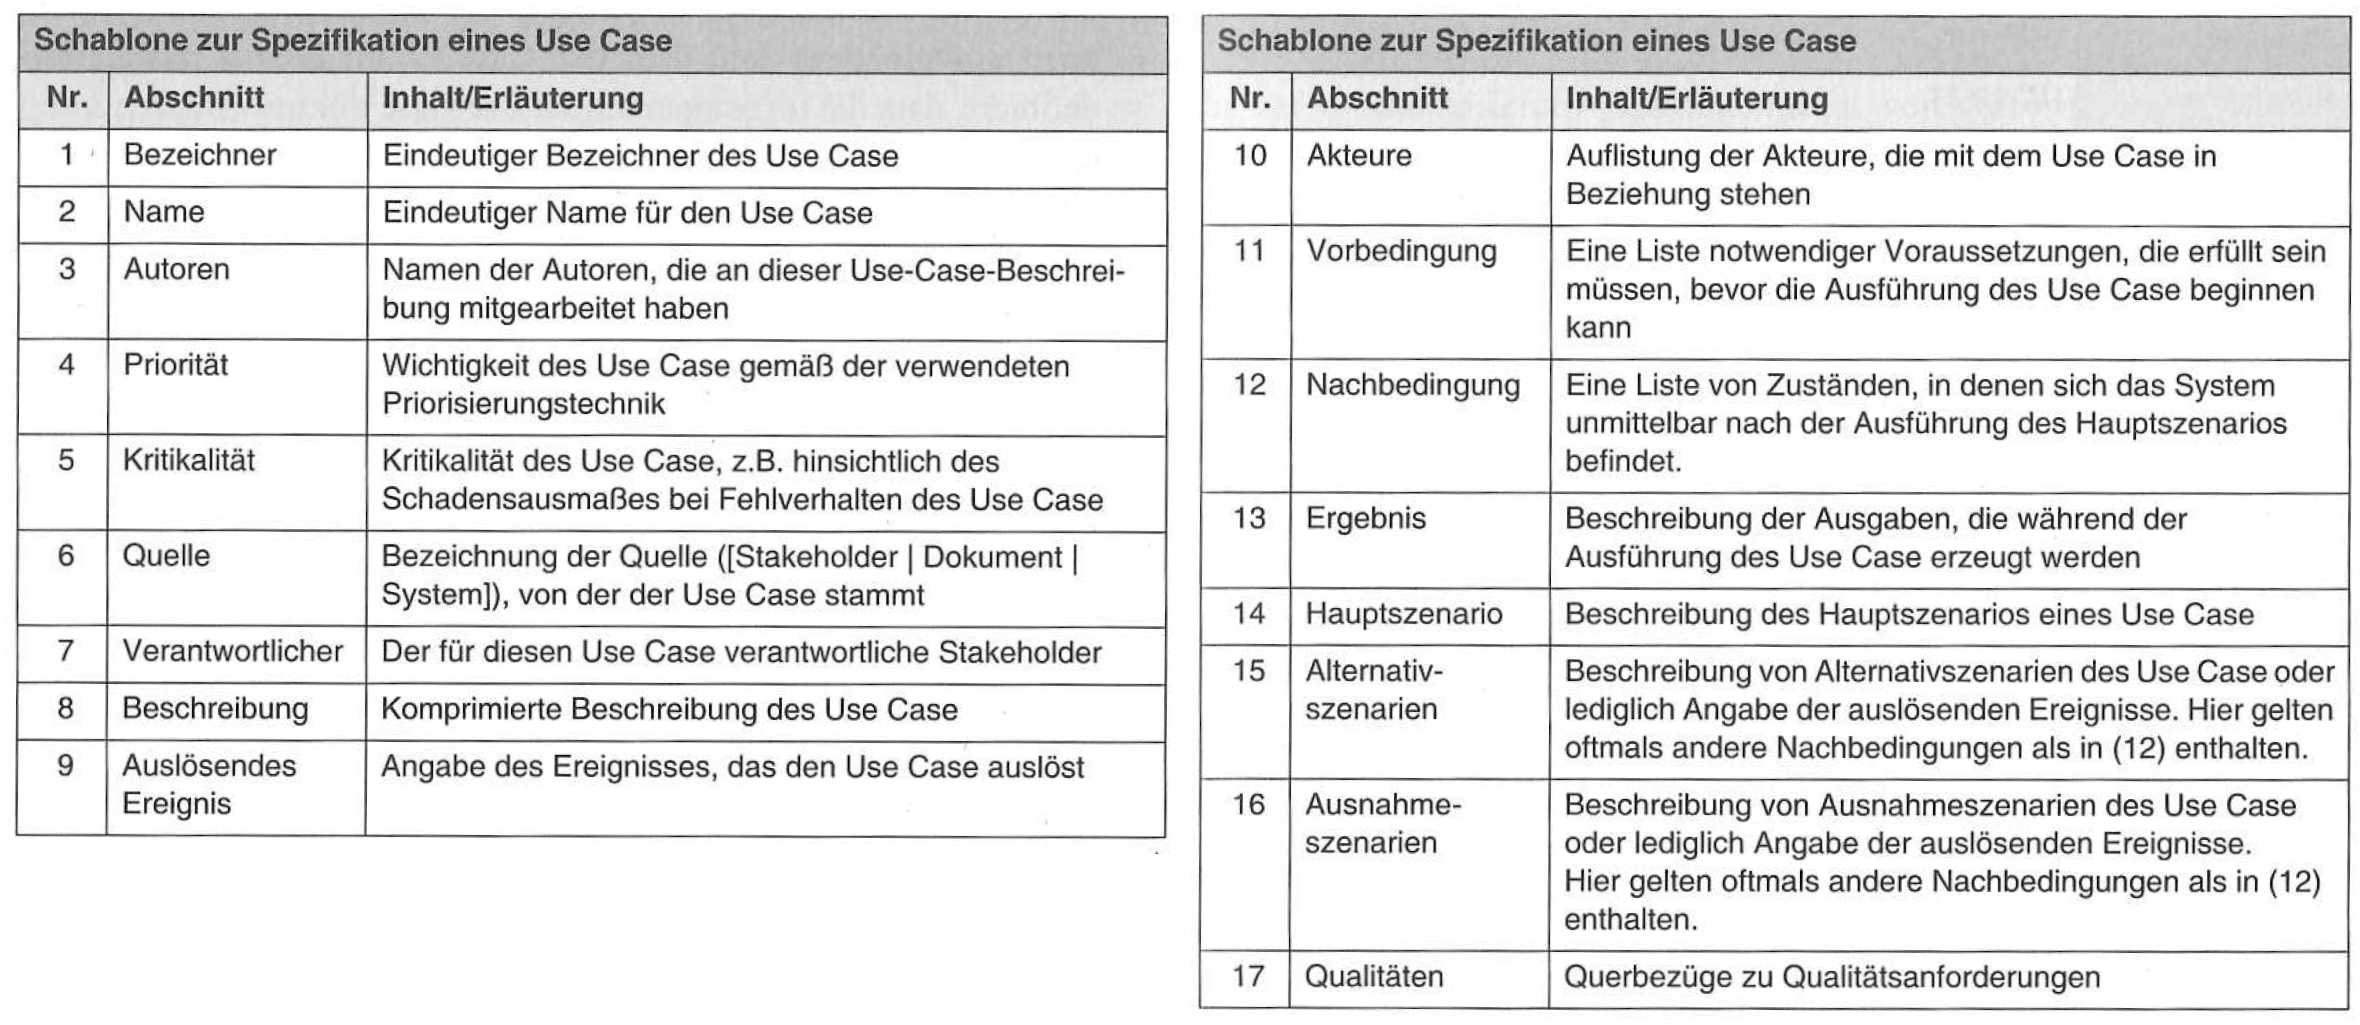
\includegraphics[scale=0.88]{Bilder/Kapitel-6/use_case_schablone.png}
		\caption[Use Case Schablone]{Use Case Schablone \cite[72 \psq]{poh15}}
		\label{fig:use_case_schablone}
	\end{addmargin*}
	\end{addmargin*}
\end{figure}

\vspace{\baselineskip} %%% für Druck

\minisec{Anwendungsfälle und User Stories}
Wir hatten in Abschnitt~\ref{sec:Kap-6.2.3} die aus dem agilen Umfeld stammenden User \mbox{Stories} angesprochen, über die sich ebenfalls die gewünschte Systemnutzung der Nutzer modellieren lässt. Anwendungsfalldiagramme und User Stories lassen sich durchaus kombinieren, zum Beispiel indem User Stories als textuelle Ergänzung zu den „Haupt“-Anwendungsfällen eines Anwendungsfalldiagramms fungieren. Wenn man den Schwerpunkt umgekehrt eher auf die User Stories setzen möchte, kann man das Anwendungsfalldiagramm als grafische Ergänzung verwenden, zum Beispiel für eine Übersicht zusammengehöriger User Stories.

\vspace{\baselineskip} %%% für Druck
\subsection{Domänenmodellierung}
\label{sec:Kap-6.3.2}

Ein Domänenmodell besteht aus statischen und dynamischen Sichten auf die Domäne. In Lektion~2 % todo Lektion~\ref{sec:Lektion-2}
haben Sie mit dem Domänenklassendiagramm eine statische Sicht auf die Domäne gesehen: Objekte bzw. Klassen, ihre Eigenschaften und Beziehungen zueinander. Im letzten Abschnitt haben Sie mit dem Anwendungsfalldiagramm Möglichkeiten kennengelernt, dynamische Aspekte der Domäne zu modellieren: Tätig\-keiten von Akteuren in der Domäne. Bisher nur ab und an kurz erwähnt, haben wir einen weiteren wichtigen Bestandteil der Domänenmodellierung, die Erstellung eines Glossars.

\vspace{2mm} %%% für Druck

\minisec{Glossar}

Ein Glossar beinhaltet Erläuterungen für das Vokabular der Domäne, das im Rahmen der Entwicklung des Softwareprodukts erläuterungsbedürftig ist. Welches 
\linebreak %%% für Druck
Vokabular der Domäne ist erläuterungsbedürftig und welches nicht? Gehören im Zoobeispiel die Tierarten ins Glossar? Bei Schaf und Ziege würden die meisten von Ihnen vermutlich nein sagen, bei Gelbzahnmeerschweinchen die meisten jedoch ja. 

\vspace{2mm} %%% für Druck

Letztendlich gibt es keine Antwort, welcher Begriff erläuterungsbedürftig ist und welcher nicht. In jedem Fall gehören alle die Objekte, Akteure, Konzepte, Tätigkeiten, Prozessverben, Zusammenhänge etc. ins Glossar, die irgendwann im Laufe des Requirements Engineering in Diskussionen mal zu Verständnisproblemen geführt haben. Das Glossar wächst also kontinuierlich an und ist im Übrigen auch nicht am Ende des Requirements Engineering zwingend abgeschlossen. In manchen Projekten werden grundsätzlich alle in Modellen und Anforderungen vorkommenden Begriffe der Domäne ins Glossar aufgenommen, dann eben auch Schaf und Ziege.

\vspace{2mm} %%% für Druck

Zu jedem Eintrag im Glossar sollten mindestens folgende Informationen enthalten sein:
\begin{itemize}
	\item der Begriff
	\item der Typ des Begriffs, z.B. ein Akteur (Nagetierpfleger) oder eine Aktion in einem Geschäftsprozess (Bonuspunkte einsetzen)
	\item die Erläuterung des Begriffs
	\item Verweise auf inhaltlich verwandte Begriffe bzw. Konzepte. Zum Beispiel beim Gelbzahnmeerschweinchen der Verweis auf den Glossareintrag des Zwergmeerschweinchens 
	\item Welche synonymen Begriffe gibt es: Synonyme sind unterschiedliche Begriffe für denselben Sachverhalt. Die Verwendung von Synonymen sollte man idealerweise ganz vermeiden. Man wird sie aber in Dokumenten und Grafiken finden, die die Stakeholder liefern. Insofern ist es wichtig, sie im Glossar aufzuführen.
	\item Handelt es sich bei diesem Begriff um ein Homonym? Ein Begriff ist ein \mbox{Homonym}, wenn er mehrere abweichende Bedeutungen hat, wie zum Beispiel die Bank, bei der ich mein Konto habe und die Bank, auf der ich im Park sitzen kann. Sofern Homonyme im Vokabular der Domäne vorkommen, empfiehlt es sich, für eine der Bedeutungen einen abweichenden Begriff zu verwenden, zum Beispiel Geldinstitut für den ersten Bank-Begriff.
	\item Ggf. Referenzen auf die Requirements Engineering-Dokumente, in denen der Begriff verwendet wird. Das ist allerdings sehr aufwändig durchzuhalten, da man das Glossar bei jedem neuen Diagramm etc. an mehreren Stellen ergänzen müsste.
\end{itemize}

\pagebreak %%% für Druck

\minisec{Die Bedeutung der Domänenmodellierung}

Das wichtigste Ziel der Domänenmodellierung ist das explizit Machen von implizitem Wissen. Betrachten Sie die folgende Aussage.

\sttpAnforderungText{Man kann Führungen durch den Zoo online buchen. Die Teilnahme an Fütterungsführungen ist aber nur für Gruppen bis 5 Personen möglich.}

\vspace{\baselineskip} %%% für Druck

Sind Führungen und Fütterungsführungen unterschiedliche Dinge? Einem Zoo-
\linebreak %%% für Druck
Domänenexperten wird das klar sein und er wird vielleicht nicht explizit darauf hinweisen. Modelliert man die Beziehung zwischen Zoobesuchern und Führungen aber in einem Domänenklassendiagramm, wird der Domänenexperte darauf hinweisen, dass die in Abbildung~\ref{fig:zoofuehrung} oben %%% links 
gezeigte Modellierung falsch ist, wenn eine Struktur wie in der unteren %%% rechten 
Hälfte der Abbildung zutrifft.

\vspace{\baselineskip} %%% für Druck
\vspace{2mm} %%% für Druck

\begin{figure}[h!]
	\centering
	
\includegraphics{Bilder/Kapitel-6/zoofuehrung_links.pdf}
	\vspace{\baselineskip}
	{\color{FernUni-MI-green}\rule{120mm}{1pt}} % horizontale farbige Linie
	\vspace{\baselineskip}
	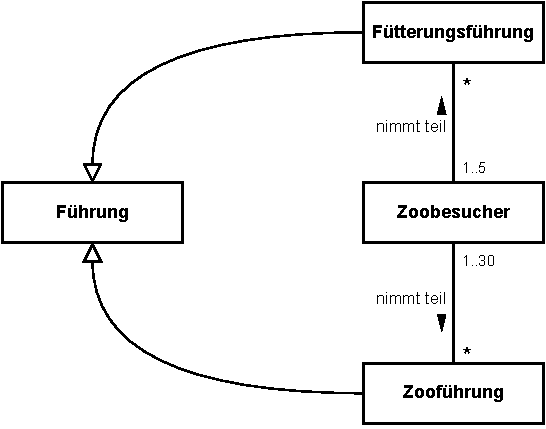
\includegraphics{Bilder/Kapitel-6/zoofuehrung_rechts.pdf}
	\caption{Zooführung}
	\label{fig:zoofuehrung}
\end{figure}

\vspace{\baselineskip} %%% für Druck

Wenn man im Requirements Engineering die Domänenmodellierung vernachlässigt, werden einem sehr sicher Anforderungen an das zu entwickelnde Softwareprodukt entgehen. Daher sollten Sie die Domäne wie einen Stakeholder behandeln und ihre „Bedürfnisse“ mit berücksichtigen. 
% 6.4
\clearpage
\section{Anforderungsvalidierung}
\label{sec:Kap-6.4}

Es geht in diesem Teilprozess darum zu analysieren, ob die bislang dokumentierten Anforderungen als Grundlage für die zu entwickelnde Software geeignet sind. \mbox{Darüber} hinaus sind natürlich die Anforderungen zu ergänzen oder zu ändern, wenn dies nicht der Fall ist; wir erhalten also (wie so oft) einen zyklischen Vorgang, der schließlich mit der Prüfung endet, dass die Anforderungen die erforderlichen Qualitäts\-kriterien erfüllen. Manchmal sagt man auch \textit{Anforderungsprüfung} zu diesem Teilprozess; dies vermeiden wir hier, weil es suggeriert, dass im Standardfall diese Prüfung positiv ausfällt und nichts zu tun ist, der Negativfall also die Ausnahme wäre. Dies ist bei der Anforderungsvalidierung nicht so. Eine Überarbeitung der Anforderungen ist der übliche Ausgang und bedeutet auch nicht, dass die Anforderungs\-ermittlung fehlerhaft durchgeführt worden wäre.

Auch der Name \textit{Anforderungsvalidierung} ist nicht genau treffend, weil er zugleich für einen Teil dieses Teilprozesses verwendet wird, wie Sie weiter unten lesen werden. Wir verwenden ihn trotzdem, weil er auch in der Literatur so vorkommt und – im weiteren Sinne – Validierung doch grob das Ergebnis dieses Teilprozesses 
\linebreak %%% für Druck
umschreibt.

Wann ist nun eine Sammlung von Anforderungen geeignet als Grundlage für die Entwicklung eines Softwaresystems? Oder umgekehrt: Was könnten Gründe dafür sein, dass Anforderungen eine zu entwickelnde Software noch unzureichend spezifizieren? Bevor wir uns mit dieser Frage näher befassen, sollten wir das hier von uns betrachtete Szenario genauer beschreiben. Aus der Diskussion über verschiedene Vorgehensmodelle wissen Sie, dass Anforderungen in den meisten Fällen zu Beginn des Softwareentwicklungsprozesses noch nicht in Gänze bekannt sind. Das Wasserfallmodell ignoriert diesen Umstand bzw. berücksichtigt ihn nur notdürftig durch eigentlich nicht vorgesehene Rücksprünge. Agile Vorgehensmodelle gehen sogar davon aus, dass anfangs wenig über die Anforderungen bekannt ist. Wir werden im Folgenden unberücksichtigt lassen, wann die Anforderungen zusammengetragen werden bzw. wie die Anforderungsermittlung mit anderen Teilprozessen verschränkt ist – je nach Vorgehensmodell kann dies sehr unterschiedlich sein. Wir abstrahieren also von allen anderen Teilprozessen bzw. ihren Aktivitäten und konzentrieren uns rein auf die Anforderungssammlung, die ja bei jedem Vorgehen irgendwann das zu erstellende System vollständig spezifiziert (sofern Anforderungen überhaupt gesammelt werden).

Wofür ist es wichtig, dass Anforderungen das zu erstellende Softwaresystem relativ genau beschreiben, also quasi ein Modell dieses Systems darstellen? Der Charakter als Modell ist bei reinem Text weniger deutlich, bei anderen, bereits genannten Spezifikationssprachen wird er deutlicher.

Der wichtigste Grund ist natürlich, dass das System auf Grundlage der Anforderungen erstellt wird. Im Idealfall liegen dem Entwicklerteam nur die Anforderungen vor, und sie haben ihren Job gut gemacht, wenn sie ein System erstellen, dass alle vorgegebenen Anforderungen erfüllt (und dies auch nachweisbar so ist). Natürlich wird es in der Realität meist weitere Anforderungen oder Aspekte geben, die implizit sowohl von den Stakeholdern gemeint waren und auch vom Entwickler berücksichtigt werden, aber nie explizit in den Anforderungen genannt wurden (implizites \mbox{Wissen}). Doch darauf kann man sich nicht verlassen! Diese impliziten Anforderungen basieren oft auf einer vertieften Branchenkenntnis oder auf Detailwissen über ein Vorgängersystem. Einem neuen Entwickler fehlt dieses implizite Wissen und er wird die Erwartungen nicht erfüllen, ohne dass man ihm einen Vorwurf machen 
\linebreak %%% für Druck
könnte.

Ein weiterer Grund ist, dass nur mit einer klaren Vorstellung über das zu erstellende Softwaresystem ein erfahrenes Softwareunternehmen ein realistisches Angebot über Zeit- und Kostenaufwand für die Erstellung des Systems machen kann. Aussagen über Kosten und Lieferzeit sind aber umgekehrt für den Kunden wichtige Informationen, die zu seiner Entscheidung beitragen, ob er die Entwicklung gemäß seiner Visionen und Ziele überhaupt in Auftrag gibt. Oft ist es so, dass in einer Verhandlungsphase die Anforderungen und die resultierenden Entwicklungskosten und -zeiten Gegenstand einer Verhandlung zwischen Auftraggeber und Auftragnehmer sind. Es ist klar, dass dafür aussagekräftige Anforderungssammlungen möglichst früh zur Verfügung stehen müssen, am besten bevor ein Entwicklungsaufwand überhaupt entsteht.

Ein dritter Grund, der aber mit dem zweiten zusammenhängt: Für jedes Software\-entwicklungsprojekt muss der Ressourcenaufwand und ein entsprechender Zeitplan existieren, damit das Softwareunternehmen realistische Versprechungen zu Liefer\-zeiten und -kosten machen kann, aber auch sein -- unterschiedlich spezialisiertes -- Personal durchgehend gewinnbringend einsetzen kann. Grundlage dafür sind zunächst die Anforderungen, die durch die zu entwickelnde Software umgesetzt 
\linebreak %%% für Druck
werden.

Was gibt es nun für Gründe, dass Anforderungen nicht ausreichen oder nicht geeignet sind, ein Softwaresystem zu spezifizieren oder, genauer, das Softwaresystem zu spezifizieren, das die Wünsche des Kunden bzw. seiner Stakeholder tatsächlich erfüllt.
\subsection{Validität}
\label{sec:Kap-6.4.1}

Wie bereits erwähnt, trägt dieser Aspekt denselben Namen wie der gesamte Teilprozess. Anforderungen sind valide, wenn sie das ausdrücken, was die Stakeholder tatsächlich gemeint haben. Man mag meinen, dass dies doch leicht zu erfüllen ist, denn die Stakeholder haben die Anforderungen ja meist direkt oder indirekt selbst formuliert. Tatsächlich geschehen aber auch dabei Fehler mit potentiell schweren Auswirkungen. Eine vergessene Negation oder eine fehlerhaft numerische Angabe können eine Anforderung stark verändern. Erfahrungsgemäß fallen derartige Fehler den Autoren der Anforderungen selbst nur selten auf. Maßnahmen der Anforderungsvalidierung sind 

\begin{itemize}
\item Gegenlesen der Anforderungen von verschiedenen Stakeholdern.
\item Plausibilitätskontrolle, also oft Einsatz des gesunden Menschenverstands.
\item Übersetzung der Anforderungen in möglichst klare, einfache Formulierungen (bei neuen Formulierungen mag auch der ursprüngliche Autor seinen Fehler leichter erkennen).

\pagebreak %%% für Druck

\item Erstellung eines Prototyps aus Teilen der Anforderungen. Dieser Ansatz wird indirekt bei agilen Verfahren durchgeführt, doch ist hier der Prototyp meist bereits der Kern des zukünftigen Softwaresystems. Ein Prototyp im eigentlichen Sinn ist aber ein Wegwerfprodukt, das hier nur der Anforderungsvalidierung dient, und meist nur die Benutzungsschnittstelle des Systems simuliert.
\item Überprüfung, ob Anforderungen sich gegenseitig widersprechen, siehe weiter unten bei „Konsistenz“.
\end{itemize}
\subsection{Konsistenz}
\label{sec:Kap-6.4.2}

Es gibt in den meisten Fällen mehrere Stakeholder mit verschiedenen Zielen und entsprechend verschiedenen Anforderungen an ein Softwaresystem. Ein Software\-system, das all diese Anforderungen erfüllt, sollte für alle Stakeholder bezüglich ihrer Ziele zufriedenstellend sein. Dies ist aber leider nicht in jedem Fall möglich, denn Stake\-holder können recht unterschiedliche Vorstellungen von dem zu entwickelnden Softwaresystem haben. Dies einerseits deshalb, weil sie sich halt verschiedene Vorstellungen gemacht haben. Oft aber ist der Grund, dass sie auch verschiedene Interessen haben und die Formulierung der Anforderungen bewusst oder unbewusst interessengeleitet ist. Als Resultat entsteht eine in sich widersprüchliche Anforderungssammlung, kein Softwaresystem kann alle Anforderungen erfüllen. Als Grundlage für den Systementwurf ist eine nicht konsistente Anforderungssammlung untauglich, denn der Entwickler müsste entscheiden, welche Anforderungen erfüllt werden sollen und welche nicht, und dafür fehlt ihm jegliche Grundlage.

Man mag einwenden, dass sich alle Beteiligten doch vorher geeinigt haben sollen, um widersprüchliche Angaben zu vermeiden. Gerade dafür sind ja auch die Vision und die Formulierung der spezifischeren Ziele da. Trotzdem ist für eine „Einigung“ die explizite und genaue Formulierung von Anforderungen Voraussetzung, und eine Vermeidung jeglicher Inkonsistenz zwischen Stakeholdern würde eine zuvor durchgeführte Anforderungssammlung erfordern – es wäre also nichts gewonnen.

Inkonsistenzen sind nicht sehr leicht zu erkennen, denn verschiedene Stakeholder verwenden oft unterschiedliche Begriffe für dieselbe Sache und formulieren ihre Anforderungen aus recht unterschiedlichen Perspektiven. Zur Identifikation von inkonsistenten Anforderungen ist es deshalb notwendig, zunächst Anforderungen so umzuformulieren, dass Gleiches gleich genannt wird (Elimination von Synonymen), Ungleiches ungleich genannt wird (Elimination von Homonymen) und die Abstraktionsebene der Anforderungsformulierungen angeglichen wird. Anschließend fallen inkonsistente Anforderungen dann gleich auf, wenn sie sich im Sinne der Logik widersprechen. Dies ist nicht immer der Fall. Auch hier ist die Verwendung eines Prototyps sinnvoll, dem Anforderungen gegenübergestellt werden. Zu widersprüchlichen Anforderungen kann es auch keinen passenden Prototypen geben.

Widersprüche in Anforderungen stellen nicht notwendigerweise widersprüchliche Vorstellungen dar. Sie können auch Hinweise darauf geben, dass einzelne Anforderungen nicht das Gemeinte ausdrücken, also nicht valide sind (\so). In diesem Fall ist die Inkonsistenz geradezu als Glücksfall anzusehen, denn sie hilft, invalide Anforderungsformulierungen zu identifizieren.
\subsection{Korrektheit}
\label{sec:Kap-6.4.3}

\vspace{-1mm} %%% für Druck

Verwandt mit der Konsistenz ist die Korrektheit. Während fehlende Konsistenz sich in Widersprüchen manifestiert, fordert Korrektheit die Einhaltung von Regeln in einem weiteren Sinn. Hierunter fällt, dass Anforderungen syntaktisch korrekt sein müssen, als natürlichsprachliche Sätze also überhaupt einen Sinn haben. Diese Regeln sind nicht übergreifend gegeben, sondern für verschiedene Entwicklungsprojekte und insbesondere für verschiedene und verschieden formalisierte Sprachen der Anforderungsermittlung unterschiedlich und unterschiedlich umfassend. Dazu gehört typischer\-weise stets syntaktische Korrektheit der jeweiligen Formulierungen bzw. Modelle aus der Anforderungsbeschreibung. Auch kann es übergreifende Regeln geben, die zum Beispiel fordern, dass verwendete Begriffe anderswo definiert sein müssen. Grundsätzlich erlaubt eine stärkere Formalisierung der Sprache für die Anforderungen mehr (sinnvolle) Regeln und damit auch mehr Möglichkeiten zur Überprüfung der Korrektheit. Diese Überprüfung wird auch \textit{Verifikation} genannt.

Für die in Lektion 3 eingeführten Petrinetze sind \zb die Regeln sinnvoll, dass man
\begin{itemize}
	\item jede Transition überhaupt jemals schalten kann, 
	\item stets einen definierten Endzustand erreichen kann,
	\item im Falle von Workflow-Netzen: dass das Netz sound ist.
\end{itemize}

Da \textit{Verifikation} und \textit{Validierung} oft verwechselt werden, hier nochmal der grundsätzliche Unterschied (der in der Literatur leider nicht konsequent Berücksichtigung findet): Bei der \textit{Verifikation} geht es nur um die Anforderungen selbst, es gibt keinen Bezug zur Realwelt. Sie kann ohne Mitwirkung der Stakeholder durchgeführt werden. Bei der \textit{Validierung} geht es ausschließlich um den Bezug der Anforderungen zur Realwelt. Sie kann ausschließlich unter Mitwirkung der Stakeholder durchgeführt werden.
\subsection{Vollständigkeit}
\label{sec:Kap-6.4.4}

\vspace{-1mm} %%% für Druck

Schließlich müssen die Anforderungen daraufhin überprüft werden, ob sie vollständig sind. Vollständig bezogen auf was? Wenn ein Stakeholder einen Wunsch vergessen hat, wird das außer ihm kaum jemandem auffallen, diese Unvollständigkeit ist hier aber nicht gemeint. Wenn „vollständig“ im Zusammenhang mit „korrekt“ gesehen wird, können in einer unvollständigen Anforderungssammlung Angaben fehlen, die im Sinne der Korrektheit zur Interpretation anderer Anforderungen notwendig sind. Derartige Lücken mögen zwar bei der Verifikation auffallen, dies ist aber nicht notwendigerweise so. Auch nicht spezifiziertes implizites Wissen gehört zu unvollständigen Anforderungssammlungen, und es fällt bei keinem der bislang genannten Schritte zwingend auf. Im Endeffekt ist es notwendig aus dem Blickwinkel eines Entwicklers, der nicht über implizites Wissen verfügt, die Anforderungen zu betrachten und zu verstehen. Auch hier ist die Konstruktion eines Prototyps hilfreich, wenigstens gedanklich. Diesmal jedoch nicht zur Rückkopplung mit den Stakeholdern, sondern zur Prüfung für den Entwickler, ob er allein aufgrund der dokumentierten Anforderungen einen Prototyp erstellen könnte. Wenn die Konstruktion aufgrund fehlender Angaben nicht möglich scheint, ist es wahrscheinlich, dass wichtige Angaben in den Anforderungen fehlen.
% 6.5
\clearpage
\section{Anforderungsmanagement}
\label{sec:Kap-6.5}

\vspace{\baselineskip} %%% für Druck

Jede Formulierung einer Anforderung, sei sie natürlichsprachlich, formalisiert sprachlich oder graphisch, wird in irgendeiner Weise als Dokument vorliegen. Da die Anforderungen Grundlage für den Softwareentwurf sind, aber auch Grundlage für ein Angebot, für einen Preis und für einen Vertrag über die Erstellung eines Software\-systems sein können, kommt ihnen organisatorisch und auch juristisch eine besondere Bedeutung zu. Auch wenn für den Entwurf stets nur die letzte Version der Anforderungen relevant ist, sollte die Entwicklung der Anforderungen systematisch festgehalten werden und Bezüge zwischen Anforderungsformulierungen sichtbar sein. Zur Motivation drei Beispiele:

\vspace{1mm} %%% für Druck

\begin{itemize}
	\item Nach Auslieferung eines Softwaresystems zeigt sich der Auftraggeber unzufrieden und beklagt, dass eine bestimmte Anforderung durch das System nicht erfüllt sei. Er verlangt Nachbesserung, die aber nur mit großem Aufwand und nicht innerhalb der gesetzten Frist möglich ist. Es kommt zum Streit. Der Auftraggeber kann tatsächlich nachweisen, dass die Anforderung von einem bestimmten Stakeholder zu einem bestimmten Zeitpunkt geäußert wurde und auch zu Protokoll genommen wurde. Allerdings hat sich bei der Anforderungsvalidierung herausgestellt, dass diese Anforderung im Widerspruch zu anderen Anforderungen gestanden hat und deshalb in Absprache mit dem Auftraggeber verändert wurde – in der veränderten Form wird sie aber tatsächlich erfüllt. Um dies alles nachvollziehen zu können, muss also auch die Historie der Anforderungen in ihren jeweiligen Formulierungen festgehalten
	\linebreak %%% für Druck
	werden.

	\vspace{1mm} %%% für Druck

	\item Das Entwicklerteam eines Softwaresystems hält eine Anforderung in ihrer mehrfach modifizierten Formulierung für unlogisch und fragt sich, ob
	\linebreak %%% für Druck
	während der Anforderungsermittlung oder -validierung ein Fehler geschehen ist. Wer mag ein Interesse an der dort formulierten Systemeigenschaft haben? Um nicht gegen die eigene Überzeugung zu entwickeln, soll nachvollzogen werden, von wem (von welchem Stakeholder) diese Anforderung eigentlich stammt. In der zuletzt abgestimmten Form hat die Anforderungssammlung keine Autoren mehr, denn sie ist in der Validierungsphase mehrfach überarbeitet worden, Anforderungen wurden kombiniert, aus komplexen Anforderungen vereinfacht, sprachlich auf eine einheitliche Abstraktionsebene gebracht usw. Um dennoch der Kernaussage der Anforderung auf den Grund gehen zu können, muss die Entwicklung der Anforderungen nachvollziehbar sein. In anderen Worten: für jede Anforderung, die während des gesamten Teilprozesses betrachtet wird, muss der Weg bis zum Ursprung (bzw. den Ursprüngen) dieser Anforderung transparent nachvollziehbar sein.

	\vspace{1mm} %%% für Druck

	\item In mehreren Anforderungen kommt derselbe Begriff vor, in einer Anforderung wird dieser Begriff im Detail erläutert. Da es sich stets um dasselbe handelt, muss das Detailwissen aus der einen Anforderung auch bei Berücksichtigung der anderen Anforderungen eingehen. Der Entwickler kann aber nicht für jeden vorkommenden Begriff alle Anforderungen im Auge haben, die damit etwas zu tun haben könnten. Er muss vielmehr darin unterstützt werden, zusammenhängende Anforderungen auch zusammen zu sehen und zu verstehen, und insbesondere entsprechende Beziehungen zwischen Anforderungen 
	\linebreak %%% für Druck
	zu erkennen.
\end{itemize}

Was folgt nun daraus für das Management der Anforderungen? Für jede Anforderung muss einerseits ihre Historie bis hin zum Ursprung nachvollziehbar sein. Dieser Ursprung besteht oft aus Textdokumenten. Aber auch Audio- und Video\-dateien sowie Dokumente anderer Dokumenttypen sind denkbar, zum Beispiel für die Doku\-mentation technischer Systeme. Idealerweise bestehen die Bezüge nicht nur aus Links auf die jeweiligen Dokumente, Dokumentnamen oder auf Orte, wo sich die Dokumente befinden, sondern geben auch an, auf welche Stelle eines Dokuments sich die Verbindung bezieht (Wo wird in einer Audio-Aufzeichnung die Anforderung erwähnt? Welches Synonym wurde durch einen neuen Begriff ersetzt?). 

\vspace{1mm} %%% für Druck

Andererseits müssen auch Querbezüge zwischen den aktuellen Dokumenten bzw. zwischen Dokumenten derselben „Generation“ festgehalten werden. Manche Anforderungen ergeben nur dann einen Sinn, wenn man sie im Zusammenhang mit einer anderen Anforderung liest, in der zum Beispiel ein verwendeter Begriff definiert und erklärt wird.

\vspace{1mm} %%% für Druck

Dies alles kann man natürlich mit einem Zettelkasten und Post-its organisieren, aber bei größeren Systemen und einer umfangreichen Anforderungssammlung ist das sicherlich keine gute Idee. Eine derartige Organisation würde zudem von einzelnen Personen abhängen, die (vielleicht) den Überblick behalten haben. Tatsächlich setzt man aber in den meisten Fällen entsprechende Content-Management Systeme ein, die Dokumente verschiedenster Typen organisieren können und die genannten Bezüge zwischen den Dokumenten und den darin verborgenen Anforderungen auf transparente Weise darstellen. Wichtig dabei ist, dass die Verwaltung und auch die Weiterentwicklung und die Modifikation all dieser Dokumente nicht von der Expertise einzelner Personen abhängen darf, die wieder – oft ungewollt und unbewusst – ihr implizites Wissen einbringen.

\vspace{1mm} %%% für Druck

Auch wenn alle Beispiele, die im Rahmen eines Universitätsmoduls vorkommen können, doch relativ klein und übersichtlich sind, ist die gedankliche Übertragung auf Systeme im Großen und die Anforderungsermittlung bei sehr vielen Stakeholdern schwierig. Bei wirklich großen Systemen ist die Ermittlung und auch die Verwaltung der Anforderungen eine äußerst komplexe und auch erfolgskritische Aufgabe, die ein hohes Maß an Professionalisierung und Automatisierung erfordert. Dies nicht zuletzt deshalb, weil sich Anforderungen auch nach Projektbeginn ändern und neue hinzukommen, und dies nicht nur bei einer agilen Vorgehensweise. Die meisten fehlgeschlagenen Großprojekte sind (wenigstens auch) an fehlerhaftem oder unzureichendem Management der Anforderungen gescheitert. Das wahrscheinlich in Deutschland bekannteste Beispiel ist der Berliner Flughafen BER, wo es allerdings nicht um ein Softwareprojekt ging. Sie können mit Internetsuche oder noch besser mit ChatGPT beeindruckende Listen von Softwareprojekten finden, die aufgrund schlechten Anforderungsmanagements nie beendet wurden, ihren Kostenrahmen deutlich überzogen haben oder erst Jahre nach der ursprünglich geplanten Auslieferung fertig
\linebreak %%% für Druck
wurden.

\pagebreak %%% für Druck

Wir alle haben zudem Erfahrungen mit Softwaresystemen gemacht, in denen wir irgendwann eine Rolle als Stakeholder gespielt haben, sei es als direkter Anwender oder anderer Nutzer. Wie oft ärgert man sich über die Schnittstelle oder die Funktionalität! Die eigenen Anforderungen, die natürlich der Entwicklung nicht zugrunde lagen, werden nicht berücksichtigt. Also wurden entsprechende Anforderungen entweder nicht erhoben oder sie sind bei dem Anforderungsmanagement unter den Tisch gefallen oder so verfälscht worden, dass sie der ursprünglichen Intention nicht mehr entsprechen.
% 6.6 kommentierte Literatur
\clearpage
\section{Kommentierte Literatur}
\label{sec:Kap-6.6}


\sttpKommLitItem{Sommerville}{2018}{Software Engineering}{som18}{Bilder/Buchcover/Buchcover_Sommerville.jpg}{}
{Kapitel 4 des Softwareengineering-Lehrbuchs beschäftigt sich überblicksartig mit vielen Aspekten des Requirements Engineering. Der Schwerpunkt liegt auf den unter\-schied\-lichen Möglichkeiten Anforderungen zu kategorisieren und den verschiedenen Techniken der Anforderungserhebung.}

\sttpKommLitItem{Broy/Kuhrmann}{2021}{Einführung in die Softwaretechnik}{bro21}{}{}
{Kapitel 5 des Lehrbuchs enthält einen knapp dreißigseitigen, gut strukturierten und verständlichen Überblick zu den wichtigsten Aspekten des Requirements Engineering. Für einen ersten Einblick in das Thema Requirements Engineering ist dieses Kapitel in Verbindung mit dem Requirements Engineering-Kapitel (Kap. 4) von \cite{som18} zu empfehlen, beide Kapitel ergänzen sich in ihren gesetzten Schwerpunkten. Kapitel 6 und 7 des Buchs von Broy/Kuhrmann vertieft auf weiteren 80 Seiten ausgewählte Aspekte und liegt vom Detailgrad zwischen \cite{som18} und \cite{poh15}.}

\sttpKommLitItem{Pohl/Rupp}{2015}{Basiswissen Requirements Engineering}{poh15}{}{}
{Begleitbuch zur Aus- und Weiterbildung zum „Certified Professional for Requirements Engineering“ von IREB (s.~S.~\pageref{sec:Kap-6:IREB}). Das Buch stellt das Thema Require\-ments Engineering sowie dessen Teilprozesse gut strukturiert und überblicksartig dar. Im Unterschied zu Lehrbüchern des Softwareengineering wie \cite{som18} und \cite{bro21} werden in diesem, knapp 150 Seiten umfassenden, rein auf Requirements Engineering fokussierten Buch, auch konkrete (praxisrelevante) Methoden in den Bereichen vorgestellt. Diese werden in der Regel zwar nicht umfassend behandelt, in der ausführ\-lichen Literaturliste des Buchs aber zahlreiche Verweise auf weiterführende \mbox{Literatur} zu diesen Methoden gegeben.}

\sttpKommLitItem{Rupp}{2014}{Requirements-Engineering und -Management}{rup14}{}{}
{Umfangreiche, sehr praxisnahe Darstellung von allen Arbeitsschritten des Requirements Engineering mit Checklisten, Schablonen und Lebensweltbeispielen. Für die konkrete Projektarbeit sehr hilfreich zur Inspiration und zum Nachschlagen verschiedener Requirements Engineering-Methoden. Um einen Überblick über das Thema Requirements Engineering insgesamt zu erhalten, ist der Inhalt zu ausführlich und zu kleinschrittig gestaltet, man verliert leicht den roten Faden. Hierfür eignet sich eher das Buch \cite{poh15}, an dem die Autorin ebenfalls mitgewirkt hat.}

\sttpKommLitItem{Bergsmann/Unterauer}{2018}{Requirements Engineering für die agile Software\-entwicklung}{ber18}{}{}
{Ausführliche und gut strukturierte Vorstellung von zahlreichen agilen Methoden für Requirements Engineering. Das Buch behandelt auch organisatorische und rechtliche Aspekte, unter anderem Aufwandsschätzung, Vertragsgestaltung und Management im agilen Requirements Engineering.}

\sttpKommLitItem{Bourque/Fairley (Hrsg.).}{2014}{SWEBOK V3.0}{swe14}{}{}
{Kapitel 1 des SWEBOK behandelt das Thema Requirements Engineering -- wie in anderen Kapiteln auf einem hohen Abstraktionsgrad. Die Begriffe dieser Lektion (Anforderung, Vision, Produktumfang etc.) kommen dort alle vor, SWEBOK kategorisiert aber anders und deutlich stärker als wir dies getan haben.}

\sttpKommLitItem{Kecher/Salvanos/Hoffmann-Elbern}{2018}{UML~2.5}{kec18}{Bilder/Buchcover/Buchcover_Kecher_Salvanos.jpg}{}
{Das schon aus anderen Lektionen bekannte UML-Buch behandelt in Kapitel 8 die UML-Anwendungsfalldiagramme. Wie immer in diesen Buch werden die Elemente des Diagramms an Lebensweltbeispielen dargestellt, die zudem teilweise schon aus den vorherigen Kapiteln des Buchs zu Objektdiagramm und Klassendiagramm bekannt sind.}